\chapter{Active Set et applications}\label{chap:nscd-act-set-appli}

\newlength\longarc
\newcommand*\Arc[2][0.3pt]{%
	\settowidth\longarc{$#2$}%
	\unitlength\longarc
	\ensuremath{\stackrel{\begin{picture}(1,0.2)\linethickness{#1}\qbezier(0,0)(0.5,0.2)(1,0)\end{picture}}{#2}}%
}



\def\BBox{\hbox{\vrule height 8pt depth 0pt width 8pt}}


\def\fl{\overrightarrow}


\newenvironment{remarque}{\textbf{Remarque:}}{}

\newlength\myindent
\setlength\myindent{2em}
\newcommand\bindent{%
  \begingroup
  \setlength{\itemindent}{\myindent}
  \addtolength{\algorithmicindent}{\myindent}
}
\newcommand\eindent{\endgroup}

\numberwithin{equation}{section}

\vspace{1cm}


\textit{Dans ce quatrième chapitre, nous proposons une implémentation de l'approche NSCD-PDAS dans le solveur d'écoulements MFiX-EXA L'objectif est de démontrer la pertinence de cette approche numérique dans un contexte applicatif. Ainsi, nous réalisons des comparaisons avec l'approche classique par éléments discrets DEM en terme de conservation d'énergie, de parallélisation et nous utilisons la méthode NSCD-PDAS pour la simulation d'un écoulement multiphasique de type lit fluidisé.}

\vspace{1cm}

\minitoc

\newpage

\section*{Introduction}

Les applications technologiques et académiques des milieux granulaires sont de tout premier ordre. L'optimisation des performances d'un lit fluidisé, l'étude du banc de sable ou la mise en oeuvre d'un ballast sur une voie ferrée sont des exemples soulignant le large spectre applicatif couvert par les milieu granulaires. Comme indiqué dans le chapitre $3$, le comportement globalisé et complexe est la résultante de phénomènes locaux et individuels combinés aux principes de Newton. Le caractère non-linéaire du contact entre particules lors des collisions est l'élément central de la complexité observable aux grandes échelles. L'étude fondamentale de ces phénomènes reste d'une complexité certaine car elle repose sur la compréhension de lois locales difficilement quantifiables et de ses répercussions sur le mouvement global. À cela, il faut intégrer les attentes de l'ingénierie telles que l'étude en géométries complexes, l'utilisation de modèles multi-physiques ou encore l'introduction d'un grand nombre de degrés de liberté. Compte tenu de tous ces éléments, inscrire la méthode NSCD-PDAS dans un cadre applicatif reste un travail complexe. C'est l'objet de ce chapitre qui présente le portage de la méthode NSCD-PDAS dans l'environnement open source MFiX-EXA. Ce choix nous permet de réaliser des comparaisons avec le modèle bien établi \textit{Méthode des éléments discrets} (DEM).\\

La DEM se démarque particulièrement par un référencement bibliographique élevé. Le mouvement du milieu granulaire est alors gouverné par la deuxième loi de Newton combinée à un modèle de contact régulier et explicite. Ce modèle de contact est à opposer un modèle non-régulier tel que traité dans les chapitres précédents. En effet, cette approche, initiée par Cundall, est populaire du fait de sa simplicité, de sa faible empreinte mémoire et de son caractère local qui la rend particulièrement adaptée au calcul parallèle. Toutefois, elle présente certaines limitations sur le pas de temps. En effet, les durées de collision, points clés de la régularisation de l'approche de Cundall, induisent des contraintes sur le pas de temps des simulations relativement restrictives lorsque les particules sont rigides. On notera par ailleurs que l'approche NSCD est implicite par essence, permettant ainsi de relaxer la contrainte sur le pas de temps, au prix d'une conceptualisation et d'une algorithmique plus complexe que la DEM.\\

Néanmoins, cette simplicité de mise en oeuvre de la DEM facilite son implémentation pour la modélisation de problèmes muti-physiques.
Le couplage de la DEM avec la simulation numérique des écoulements, ou Computational Fluid Dynamics (CFD), illustre particulièrement ce point.
Cette approche mixte Lagrangienne/Eulérienne a permis dès le début des années 90 de simuler/modéliser la dynamique de lits fluidisés par exemple \cite{tsuji1992lagrangian,tsuji1993discrete,tsuji2010simultaneous,liu2011simulation,ku2015cfd}. De même le caractère local et explicite de la DEM a facilité et favorisé la parallélisation de cette approche. Cette tendance s'observe par le biais des solveurs commerciaux et open source qui font référence. Dans cette optique, plusieurs outils numériques de prédiction d'écoulements granulaires existent. Parmi les plus populaires on note YADE-OPEN DEM, qui offre un framework open source extensible pour les modèles numériques discrets, axé sur la DEM (\cite{vsmilauer2010yade, kozicki2009yade}), tout comme LIGGGHTS\cite{goniva2010open}. Le couplage fluide avec le milieu granulaire s'obtient en couplant deux codes différents comme OpenFOAM + LIGGGHTS ou ANSYS CFD avec le logiciel EDEM \cite{spogis2008multiphase}. La stratégie d'unifier dans le même code les solveurs fluides et granulaires est observée pour le solveur parallèle NGA \cite{desjardins2008high}, ou encore les travaux portant sur l'inclusion de solveurs granulaires dans des codes volumes finis pour la simulation d'écoulements turbulents réactifs, comme c'est le cas du code YALES2 développé au laboratoire CORIA (COmplexe de Recherche Interprofessionnel en Aérothermochimie) \cite{moureau2011design, dufresne2020massively}. MFiX-EXA \cite{gopalakrishnan2013development} quant à lui, est un logiciel open source orienté vers le dimensionnement de procédés industriels de traitement des gaz et de capture de CO2 à l'échelle du prototypage.
Ceci implique des développements méthodologiques intégrants couplages multiphysiques et calcul massivement parallèle \cite{musser2021mfix}.\\

Dans le registre de l'interaction fluide-milieu granulaire, on notera les articles de Dbouk, Perales \textit{et al.} \cite{dbouk2016df} sur la plateforme numérique Xper (eXtended cohesive zone models and PERiodic homogenization) dédiée à la gestion du contact frottant entre particules en présence de fluide. Cette plateforme repose sur le couplage du logiciel libre LMGC90 (Logiciel de Mécanique Gérant le Contact écrit en Fortran 90) \cite{dubois2013lmgc90} conçu pour faciliter les couplages avec d'autres codes de calcul et de la bibliothèque PELICANS pour la résolution des comportements volumiques des corps (Éléments finis ou Volumes finis), permettant ainsi de s'intéresser à une large gamme de problématiques issus d'applications industrielles\footnote{http://mimetics-engineering.fr/index.php/lmgc90/}. Le traitement des collisions résultant de la physique granulaire est fait avec l'approche de modélisation par éléments discrets NSCD implémentée dans le code LMGC90.\\

Dans ce contexte, on se propose d'implémenter le formalisme numérique NSCD-PDAS dans le logiciel open source MFiX-EXA. L'idée sous-jacente est de pouvoir hériter du parallélisme et du couplage fluide-particules de MFiX-EXA afin d'évaluer la pertinence de l'approche NSCD-PDAS dans ce contexte industriel. Ce choix est motivé par la possibilité de comparer NSCD et DEM dans le cadre du calcul parallèle et la possibilité de traiter les écoulements fluide granulaires. Pour cela, nous allons introduire ce chapitre par un rappel de l'approche DEM-CUNDALL et des lois gouvernant la dynamique des milieux granulaires. Ensuite, nous nous intéresserons au solveur multiphasique MFiX-EXA en décrivant brièvement l'algorithme de résolution implémenté pour l'étude des interactions fluides-particules et particules-particules. Une section sera dédiée à la présentation de la stratégie de parallélisation dans MFiX-EXA, puis à l'implémentation et l'adaptation du formalisme NSCD-PDAS dans ce solveur. Enfin, la dernière partie de ce chapitre sera entièrement consacrée aux simulations numériques d'écoulements granulaires purs et couplés au fluide, en confrontant les résultats obtenus par NSCD-PDAS à ceux obtenus avec le modèle DEM-CUNDALL.

\section{Modélisation discrète et solveur granulaire}

Après avoir introduit le chapitre par une description de la modélisation discrète DEM et de ses objectifs dans le cadre industriel, nous allons nous intéresser dans cette première partie au modèle mathématique, avant d'introduire le modèle de contact utilisé et son implémentation dans le solveur MFiX-EXA.

\subsection{Loi de Newton et description des équations de mouvement}

La description macroscopique du mouvement d'un milieu granulaire peut s'obtenir par la résolution des équations classiques de la mécanique, à savoir la seconde loi de Newton. La particule est soumise à des forces dites de volumes et de contacts. Considérons donc dans ce qui suit, $N$ particules sphériques, chacune ayant un diamètre $D$ et une densité $\rho$. Ces $N$ particules sont représentées dans un référentiel à l'instant $t$ par ${(\vect{X}^{(i)}(t),\vect{V}^{(i)}(t), \vect{\omega}^{(i)}(t), D^{(i)}, \rho^{(i)}, i = 1 ... N)}$, où $\vect{X}^{(i)}(t)$ désigne la position de la $i^{eme}$ particule, $\vect{V}^{(i)}(t)$ et $\vect{\omega}^{(i)}(t)$ désignent ses vitesses linéaires et angulaires, $D^{(i)}$ indique son diamètre et $\rho^{(i)}$ représente sa densité. La masse $m^{(i)}$ et le moment d'inertie $I^{(i)}$ de la $i^{eme}$ particule sont égaux à $\rho^{(i)} \frac{\pi D^{(i)3}}{6}$ et $m^{(i)} \frac{D^{(i)2}}{10}$, respectivement. La position, les vitesses de translation et les vitesses angulaires de la $i^{ème}$ particule évoluent selon la loi de Newton:

\begin{equation} \label{eq_solide1}
\frac{d}{dt} \vect{X}^{(i)}(t) = \vect{V}^{(i)}(t)
\end{equation}

\begin{equation} \label{eq_solide2}
m^{(i)} \frac{d}{dt} \vect{V}^{(i)}(t) = \vect{F}_T^{(i)} = m^{(i)} \vect{g} + \vect{F}_d^{(i)}(t) + \vect{F}_c^{(i)}(t)
\end{equation}

\begin{equation} \label{eq_solide3}
I^{(i)} \frac{d}{dt}\vect{\omega}^{(i)}(t) = T^{(i)}
\end{equation}

où $\vect{g}$ est l'accélération due à la pesanteur, $\vect{F}_d^{(i)}(t)$ est la force de traînée totale (pression et viscosité que l'on verra en détail dans la section \ref{section_fluide}) s'exerçant sur une particule se situant dans une cellule fluide, $\vect{F}_c^{(i)}(t)$ la force de contact nette résultant du contact avec d'autres particules, $T^{(i)}$ la somme de tous les couples agissant sur la $i^{eme}$  particule, et $\vect{F}_T^{(i)}$ est la somme totale de toutes les forces agissant sur la $i^{eme}$ particule. Ce qui nous amène à décrire les modèles associés à la mécanique du contact.

\subsection{Cundall et la régularisation du contact}

Les milieux granulaires sont caractérisés par de nombreux contacts simultanés, et dans le cadre de l'approche par éléments discrets, ceux-ci sont résolus contact par contact directement à l'aide d'un modèle à "Sphères souples" (Soft-Sphere model en anglais). Les forces d'interactions sont exprimées sur la base du modèle "Ressort-Amortisseur" (Spring-Dashpot model) de Cundall et Strack (1979) \cite{cundall1979discrete}, considéré comme la première technique de simulation de la dynamique des milieux granulaires publiée dans la littérature. Dans une telle approche, les particules restent parfaitement rigides et indéformables, mais elles ont la possibilité de s’interpénétrer très légèrement. Ces interpénétrations sont alors utilisées pour calculer une force répulsive proportionnelle à l'interpénétration qui tend à s'y opposer. Avant de décrire ce modèle de contact, intéressons nous à la description géométrique du contact entre 2 particules.

\subsubsection{Description géométrique du contact}

Dans ce paragraphe, nous allons décrire le modèle cinématique qui régit la dynamique de chaque particule du milieu. Pour des raisons de simplicité, nous nous limitons au cas d'un contact entre deux particules sphériques bidimensionnels $i$ et $j$ en contact, à diamètres égaux à $D^{(i)}$ et $D^{(j)}$, situées à $\vect{X}^{(i)}$ et $\vect{X}^{(j)}$. La particule $i$ se déplace avec des vitesses linéaire et angulaire égales à $\vect{V}^{(i)}(t)$ et $\vect{\omega}^{(i)}(t)$, respectivement. De même, la particule j se déplace avec des vitesses linéaire et angulaire égales à $\vect{V}^{(j)}(t)$ et $\vect{\omega}^{(j)}(t)$, respectivement. On définit alors le chevauchement normal ou la distance d'interpénétration entre les particules en contact par la formule suivante:

\begin{equation} \label{eq: 1}
\delta_n = 0,5 (D^{(i)} + D^{(j)}) - |\vect{X}^{(i)} - \vect{X}^{(j)}|
\end{equation}

\noindent Lorsque $\delta_n > 0$, les particules ne sont pas en contact et il n'y a pas de force de répulsion qui est exercée. Dès que $\delta_n$ devient négatif, il y a interpénétration, et une force de répulsion tend à les séparer.

\begin{figure}[!h]
        \centering
        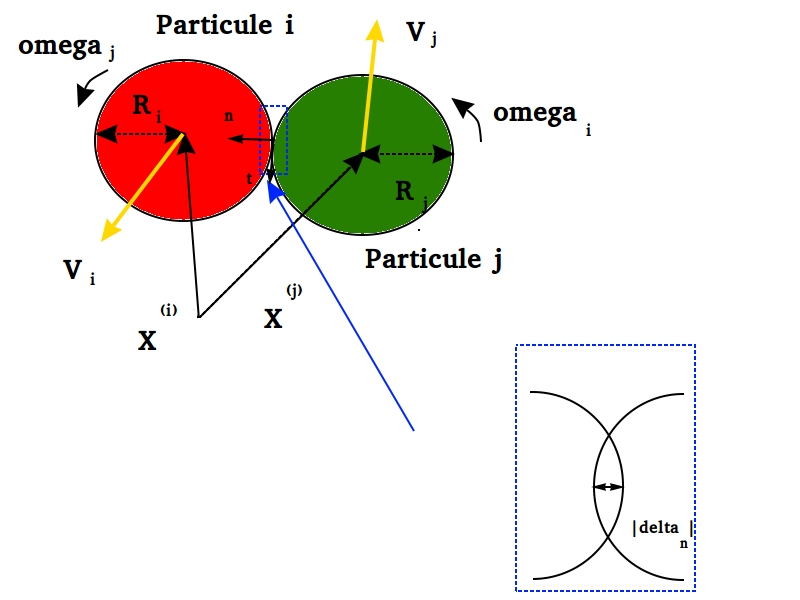
\includegraphics[width=0.7\textwidth]{chapitres/chapitre_4/figures/schematic_2_particles.jpg}
        \caption{Schéma de deux particules i et j en contact.}
        \label{fig1}    
    \end{figure}


Le vecteur unitaire le long de la ligne de contact pointant de la particule $i$ à la particule $j$ est

\begin{equation} \label{eq: 2}
\vect{\eta}_{ij} = \frac{\vect{X}^{(j)} - \vect{X}^{(i)}}{|\vect{X}^{(j)} - \vect{X}^{(i)}|}
\end{equation}

et la vitesse relative du point de contact devient

\begin{equation} \label{eq: 3}
\vect{V}^{(ij)} = \vect{V}^{(i)} - \vect{V}^{(j)} + ( L^{(i)} \vect{\omega}^{(i)} + L^{(j)} \vect{\omega}^{(j)} ) \wedge \vect{\eta}_{ij}
\end{equation}

où $L^{(i)}$ et L$^{(j)}$ sont la distance entre le point de contact et le centre de la particule $i$ et $j$, respectivement. Ils sont donnés par

\begin{equation} \label{eq: 4}
L^{(i)} = \frac{|\vect{X}^{(j)} - \vect{X}^{(i)}|^2 + r_i^2 - r_j^2}{2|\vect{X}^{(j)} - \vect{X}^{(i)}|}
\end{equation}

avec $r^{(i)}$ et $r^{(j)}$ les rayons des particules $i$ et $j$, et

\begin{equation} \label{eq: 5}
L^{(j)} = |\vect{X}^{(j)} - \vect{X}^{(i)}| - L^{(i)}
\end{equation}

Les composantes normales et tangentielles de la vitesse de contact, $\vect{V}_{(nij)}$ et $\vect{V}_{(tij)}$ respectivement, sont

\begin{equation} \label{eq: 6}
\vect{V}_{(nij)} = (\vect{V}^{(i)} - \vect{V}^{(j)}) . \vect{\eta}_{ij} \vect{\eta}_{ij},
\end{equation}

et

\begin{equation} \label{eq: 7}
\vect{V}_{(tij)} = \vect{V}^{(ij)} - \vect{V}^{(ij)} . \vect{\eta}_{ij} \vect{\eta}_{ij}
\end{equation}

La tangente au plan de contact $t_{ij}$ est

\begin{equation} \label{eq: 8}
t_{ij} = \frac{\vect{V}_{(tij)}}{|\vect{V}_{(tij)}|}
\end{equation}

\subsubsection{Modèle de contact Ressort-Amortisseur}

 Il s'agit ici de présenter le modèle de contact Ressort-Amortisseur \cite{hu2010determination}. Avec ce modèle, une collision particule-particule est traitée comme un processus continu qui se produit sur une période de temps finie, la force de contact étant calculée comme une fonction continue de la distance entre les particules en contact et reposant sur des lois d'interaction empiriques caractérisées par la constante de raideur normale du ressort, la constante de dissipation et le coefficient de frottement. Le chevauchement entre les deux particules en contact est représenté par un système de ressorts et d'amortisseurs (voir Figure \ref{fig2}) dans les directions normale et tangentielle. Le ressort assure la répulsion des particules en contact et l'amortisseur imite la dissipation de l'énergie cinétique due aux collisions inélastiques. La constante de raideur normale de contact, notée $k_n$, correspond à la raideur du ressort étend au moment du contact. Cette constante est avant tout un paramètre numérique, et non pas un paramètre physique représentant le comportement local de la particule. On parle aussi de "paramètre de régularisation" ou de "pénalisation de contact". Cette régularisation de contact dans la direction normale est également appliquée dans la direction tangentielle, d'où l'introduction d'une seconde constante, la raideur tangentielle $k_t$. Ces constantes doivent être choisies suffisamment grandes pour que le chevauchement entre particules en contact reste faible par rapport à leur diamètre. De même, les coefficients d'amortissement visqueux au contact appliquent une force proportionnelle à la vitesse, dans les directions normales et tangentielles opposées au mouvement, notées respectivement $\eta_{t}$ et $\eta_{n}$. 

\begin{figure}[!h]
        \centering
        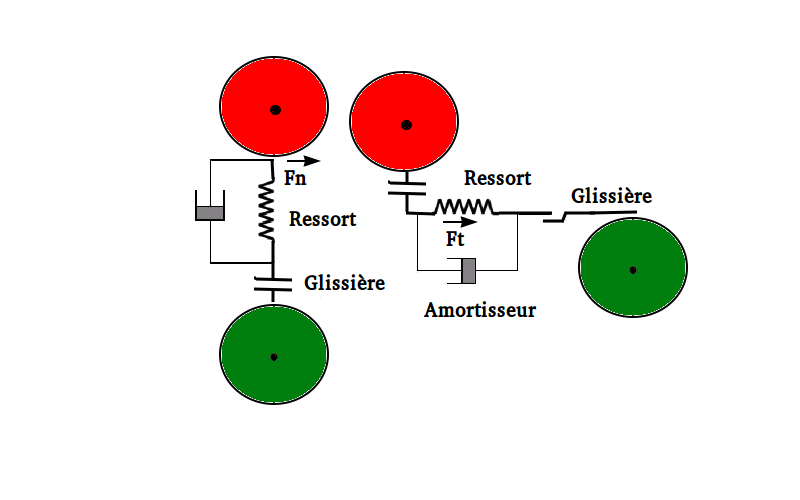
\includegraphics[width=0.8\textwidth]{chapitres/chapitre_4/figures/schematic_spring_dashpot.png}
        \caption{Modèle de contact Ressort-Amortisseur utilisé pour modéliser les forces de contact entre deux particules i et j dans une approche à sphère souple.}
        \label{fig2}    
    \end{figure}

Les composantes normales et tangentielles de la force de contact $\vect{F}_{ij}$, au temps $t$, sont décomposées en une force conservatrice du ressort $F^S_{ij}$ et une force dissipative  d'amortissement $F^D_{ij}$

\begin{equation} \label{eq: 9}
\vect{F}_{nij}(t) = \vect{F}^S_{nij}(t) + \vect{F}^D_{nij}(t),
\end{equation}

et

\begin{equation} \label{eq: 10}
\vect{F}_{tij}(t) = \vect{F}^S_{tij}(t) + \vect{F}^D_{tij}(t)
\end{equation}

L'effort normal du ressort $F^S_{nij}$ est calculé sur la base du chevauchement $\delta_n$ entre les particules. Il est donné par:

\begin{equation} \label{eq: 11}
\vect{F}^S_{nij} = - k_n \delta_n \vect{\eta}_{ij}
\end{equation}

L'effort tangentiel du ressort est nul lorsque le contact est initié. Ensuite, à chaque instant, il est donné par:

\begin{equation} \label{eq: 12}
\vect{F}^S_{tij} = - k_t \delta_t
\end{equation}

où $\delta_t$ représente le déplacement tangentiel. A l'initialisation du contact, le déplacement tangentiel est calculé comme suit:

\begin{equation} \label{eq: 13}
\delta_t = \vect{V}_{tij} min(\frac{|\vect{\delta}_n|}{\vect{V}_{ij}.\vect{\eta}_{ij}},\Delta t),
\end{equation}

\noindent à l'instant $t + \Delta t$, le déplacement tangentiel est calculé de la façon suivante:
%
\begin{equation} \label{eq: 14}
\vect{\delta}_t(t + \Delta t) = \vect{\delta}_t(t) + \vect{V}_{ij} \Delta t
\end{equation}

Dans l'expression ci-dessus, le déplacement tangentiel accumulé $\delta_t(t)$ à l'instant $t$ ne se situera pas nécessairement sur le plan tangent à l'instant $t + \Delta t$. Par conséquent, l'expression ci-dessus pour le déplacement tangentiel est corrigée afin de garantir que le déplacement tangentiel se situe dans le plan tangent. La correction est obtenue en soustrayant la composante normale $\delta_t(t + \Delta t)$, soit:

\begin{equation} \label{eq: 15}
\vect{\delta}_t(t + \Delta t) =  \vect{\delta}_t(t + \Delta t) - (\vect{\delta}_t(t + \Delta t).\vect{\eta}_{ij}) \vect{\eta}_{ij}
\end{equation}

Pour l'effort tangentiel dû au frottement de Coulomb, si l'expression suivante est vérifiée pendant le contact:

\begin{equation} \label{eq: 16}
|\vect{F}_{tij}| > \mu |\vect{F}_{nij}|
\end{equation}

\noindent alors le frottement a un statut glissant et la force de contact tangentielle est donnée par:

\begin{equation} \label{eq: 17}
\vect{F}_{tij} = \left\{
    \begin{array}{ll}
        - \mu |\vect{F}_{nij}|t_{ij} & \mbox{si } \vect{t}_{ij} \ne 0 \\
        - \mu |\vect{F}_{nij}|\frac{\delta_t}{\delta_t|} & \mbox{si } \vect{t}_{ij} = 0, \vect{\delta}_t \ne 0 \\
        0 & \mbox{sinon.}
    \end{array}
\right.
\end{equation}

Il est important de noter que la $i^{eme}$ particule de la paire de contact $(i,j)$ subit une force de contact égale à $\vect{F}_{ij}$ et que la $j^{eme}$ particule, selon la troisième loi du mouvement de Newton, subit une force de contact égale et opposée (c.-à-d. $-\vect{F}_{ij}$). Par conséquent, la force de contact totale $F^i_{c}(t)$ à tout moment sur la particule est donnée par:

\begin{equation} \label{eq: 18}
\vect{F}^i_{c}(t) = \sum_{i=1,i \ne j}^N (\vect{F}^S_{ij}(t) + \vect{F}^D_{ij}(t)), 
\end{equation}

et le couple total agissant sur la $i^{eme}$ particule est calculé par

\begin{equation} \label{eq: 19}
\vect{T}_{i}(t) = \sum_{i=1,i \ne j}^N (L^{(i)} \vect{\eta}_{ij} \wedge \vect{F}_{tij}(t))
\end{equation}

\subsubsection{Modèle de contact Hertzien}

Comme le modèle Ressort-Amortisseur, le modèle de contact Hertzien autorise les déformations et l'interpénétration lors du contact et permet de traiter les contacts de façon explicite suivant la loi de Hertz régularisante. On parle alors de modèles de contact régulier.\\
Dans le cadre d'un contact faisant intervenir deux particules $i$ et $j$ appartenant à deux phases solides différentes, notées $m$ et $l$, le modèle de contact Hertzien permet de déterminer les raideurs de ressort normale et tangentielle à partir du module de Young et du coefficient de Poisson comme suit:

\begin{equation} \label{eq: 20}
K_{n,ij} = \frac{4}{3} \frac{E_m E_l \sqrt{r^*_{ml}}}{E_m (1 - \sigma_l^2) + E_l (1 - \sigma_m^2)}\delta^{\frac{1}{2}}_{n,ij},
\end{equation}

\begin{equation} \label{eq: 21}
K_{t,ij} = \frac{16}{3} \frac{G_m G_l \sqrt{r^*_{ml}}}{G_m (2 - \sigma_l) + G_l (2 - \sigma_m)}\delta^{\frac{1}{2}}_{n,ij},
\end{equation}

où $E_m$ et $E_l$ sont les modules de Young et $\sigma_m$ et $\sigma_l$ sont les ratios de Poisson des deux phases solides. $G_m$, $G_l$ sont les modules de cisaillement calculés avec $G_m = \frac{E_m}{2(1 + \sigma_m)}$, $G_l = \frac{E_l}{2(1 + \sigma_l)}$ et $\frac{1}{r^*_{ml}} = \frac{1}{r_{(m)}} + \frac{1}{r_{(l)}}$.

\subsection{Discrétisation temporelle des équations de mouvement}

La première étape de la simulation des milieux granulaires est la discrétisation temporelle des équations régissant le mouvement des particules. Une modélisation par DEM est basée sur une intégration temporelle. Le schéma utilisé par défaut dans le solveur granulaire MFiX-DEM est un schéma de premier ordre de type "saute-mouton". Dans ce schéma, la position du centre, la vitesse de translation, et la vitesse angulaire de la particule à l'instant $(t + \Delta t)$ sont obtenues à partir des valeurs à l'instant $t$ par

\begin{equation} \label{eq: 22}
\vect{V}^{(i)}(t+\Delta t) = \vect{V}^{(i)}(t) + \frac{\vect{F}_T^{(i)}(t)}{m^{(i)}}\Delta t,
\end{equation}

\begin{equation} \label{eq: 23}
\vect{X}^{(i)}(t+\Delta t) = \vect{X}^{(i)}(t) + \vect{V}^{(i)}(t+\Delta t) \Delta t,
\end{equation}

\begin{equation} \label{eq: 24}
\vect{\omega}^{(i)}(t+\Delta t) = \vect{\omega}^{(i)}(t) + \frac{\vect{T}^{(i)}(t)}{I^{(i)}}\Delta t
\end{equation}

\noindent respectivement, où $\vect{F}_T^{(i)}(t)$ et $T^{(i)}$ représentent la force totale et le couple agissant sur la particule.\\

D'autres schémas d'intégrations peuvent également être utilisés, tel que le schéma de second ordre Adams-Bashforth. Dans ce schéma, la vitesse de translation, la position du centre de la particule et la vitesse angulaire à l'instant $(t + \Delta t)$ sont obtenues à partir des valeurs à l'instant $t$ et également de $(t - \Delta t)$ par

\begin{equation} \label{eq: 25}
\vect{V}^{(i)}(t+\Delta t) = \vect{V}^{(i)}(t) + \frac{0.5}{m^{(i)}}(3 \vect{F}_T^{(i)}(t) - \vect{F}_T^{(i)}(t- \Delta t))\Delta t,
\end{equation}

\begin{equation} \label{eq: 26}
\vect{X}^{(i)}(t+\Delta t) = \vect{X}^{(i)}(t) + 0.5(3 \vect{V}^{(i)}(t) - \vect{V}^{(i)}(t- \Delta t))\Delta t,
\end{equation}

\begin{equation} \label{eq: 27}
\vect{\omega}^{(i)}(t+\Delta t) = \vect{\omega}^{(i)}(t) + \frac{0.5}{I^{(i)}}(3T^{(i)}(t) - T^{(i)}(t- \Delta t))\Delta t,
\end{equation}

\noindent respectivement. Ce schéma requiert donc une connaissance des valeurs au pas de temps précédent $(t- \Delta t)$, ce qui le rend plus coûteux en mémoire comparé au schéma d'ordre 1.

\subsection{Présentation du solveur multiphasique MFiX-EXA}

MFiX "Multiphase Flow with Interphase eXchange" est un solveur open source d’écoulements multiphasiques en dynamique des fluides numérique \cite{garg2012documentation}, développé par le Laboratoire national de la technologie de l’énergie (NETL). Ce solveur est utilisé par une grande communauté de scientifiques, principalement aux Etats-Unis, pour simuler les écoulements dans les procédés industriels. D'un point de vue modélisation, deux approches y sont implémentées, à savoir l'approche deux fluides "Two-Fluid Model" (TFM) de type Euler-Euler qui considèrent les deux phases fluide et solide comme un ensemble homogène, et l'approche Euler-Lagrange qui permet de calculer l'écoulement du fluide en traitant séparément la phase fluide continue de la phase solide constituée de l'ensemble des particules, modélisé par la méthode des éléments discrets (DEM). Nous reviendrons sur ces deux approches en détail dans les sections suivantes. MFiX-DEM représente la partie du solveur qui traite l'écoulement granulaire pur du solveur MFiX, et permet, d’une part, de modéliser le comportement dynamique de chaque particule solide suivant la seconde loi de Newton relative au mouvement, et d’autre part, de traiter l'écoulement de la phase fluide. Pour la partie DEM, ce sont exactement les équations (\ref{eq_solide1}) -- (\ref{eq: 27}) précédemment présentées qui y sont implémentées.\\
Dans ce type de solveur, deux éléments sont importants d'un point de vue coût de calcul; d'une part la recherche de voisin, et d'autre part le parallélisme. Nous allons dans un premier temps décrire brièvement l'algorithme de résolution du solveur granulaire implémenté dans MFiX-EXA.

\subsubsection*{Algorithme global de résolution du solveur MFiX-DEM}

\begin{algorithm}[H]
 \SetAlgoLined % new in release 4.01 (Dec 2009); doesn't work in release 3.9 (Oct 2005)
 \KwData{Positions et vitesses des particules, conditions aux limites du domaine de calcul}
 \KwResult{Résolution des contacts}
 \For{chaque itération temporelle}{
  Localisation des positions des particules\;
  Détection des voisins et Construction de la liste des contacts\;
  Calcul des forces de contacts\;
  Actualisation des nouvelles positions et vitesses\;
 }
 \caption{Algorithme MFiX-DEM.}
\end{algorithm}
\vspace{0.2cm}
Pour simplifier, nous nous limitons à la description du solveur DEM sans évoquer le couplage avec le solveur fluide. A chaque itération temporelle, le solveur MFiX-DEM entame le processus de résolution des contacts. Les positions et vitesses des particules ainsi que les conditions aux limites du domaine de calcul sont lues par MFiX. Une fois que ces données sont vérifiées, MFiX fait appel à la routine d'avancement temporel pour calculer les nouvelles valeurs mises à jour pour chaque particule via l'itération suivante. Cette routine lance à son tour une séquence d'appels à plusieurs autres routines, la première permet de localiser chaque particule, puis une seconde routine est appelée pour déterminer la liste des voisins potentiels de chaque particule suivant l'algorithme de recherche de voisins. Une troisième routine permet de calculer les forces de contacts et de frottement (éventuellement les forces de traînées en présence d'un couplage CFD-DEM), puis une dernière routine permet d'intégrer les informations de toutes les routines précédemment appelées et de calculer les nouvelles positions et vitesses relatives aux particules selon le schéma d'intégration en temps utilisé (Euler explicite ou Adams Bashforth). Les étapes de résolution des contacts ainsi que les différentes routines appelées par le solveur MFiX-DEM sont résumées dans le schéma ci-dessous:

\begin{figure}[!h]
        \centering
        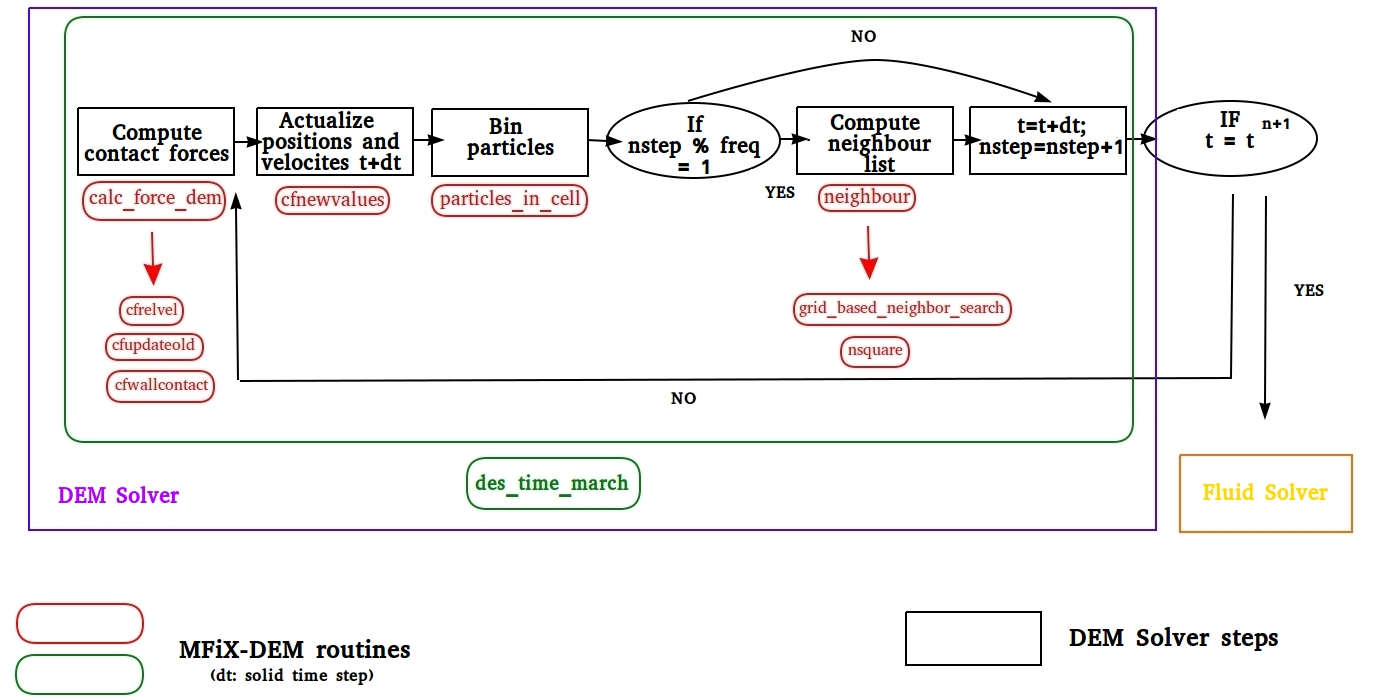
\includegraphics[width=1.0\textwidth]{chapitres/chapitre_4/figures/dem_solver_scheme.jpg}
        \caption{Routines d'appel du solveur MFiX-DEM pour la résolution des contacts.}
        \label{fig6}    
    \end{figure}

\subsubsection*{Recherche de voisins dans MFiX-DEM}

Dans un contexte de collisions entre particules, en préliminaire du calcul des forces de contacts régissant la dynamique dans ces milieux, il est primordial de connaître, à chaque pas de temps, les particules potentiellement susceptibles de rentrer en collision. La recherche des plus proches voisins est une des composantes de toute simulation en milieu granulaire. Le problème consiste à trouver l'ensemble des $k$ plus proches voisins d'une particule dans un ensemble de particules. Pour cela, quatre algorithmes de recherche de voisins sont implémentés dans MFiX-DEM. L'algorithme de recherche \textit{"Nsquare"} $N^2$, $N$ étant le nombre total de particules dans le domaine, les algorithmes \textit{"Quadtree"} et \textit{"Octree"}, et l'algorithme \textit{"Cell-linked list"}. Ce dernier, imaginé par Verlet \cite{verlet1967computer}, consiste à discrétiser le domaine de calcul en cellules pour former une grille de détection, puis à partir des coordonnées de chaque particules de la grille, identifier les contacts potentiels de la particule d'intérêt se trouvent dans une cellule centrale en itérant uniquement sur les cellules adjacentes. Comme le montre le schéma $2D$ de la Figure \ref{fig5}, si la particule d'intérêt est celle représentée par la particule rouge, alors les particules appartenant à $8$ cellules adjacentes $+1$ pour la cellule centrale ($26$ dans le cas $3D$ $+1$ pour la cellule centrale), ainsi que les particules appartenant à la même cellule que la particule d'intérêt (particules oranges), sont considérées comme des voisins potentiels. Ainsi, seules ces particules sont ensuite comparées à la particule d'intérêt pour un contact voisin. Les seuls calculs de distance à effectuer concernent les voisins potentiels, ce qui permet un gain en temps de calcul. Quelque soit la méthode de recherche, deux particules $i$ et $j$ situées en $X(i)$ et $X(j)$ et ont les rayons $R_i$ et $R_j$, sont considérés comme voisins s'ils satisfont à la condition suivante:

\begin{equation} \label{eq: 1}
|\vect{X}^{(i)} - \vect{X}^{(i)}| < K (R_i + R_j),
\end{equation}

\noindent où $K$ est un paramètre d'entrée utilisateur qui permet de construire la liste des voisins de chaque particule.

\begin{figure}[!h]
        \centering
        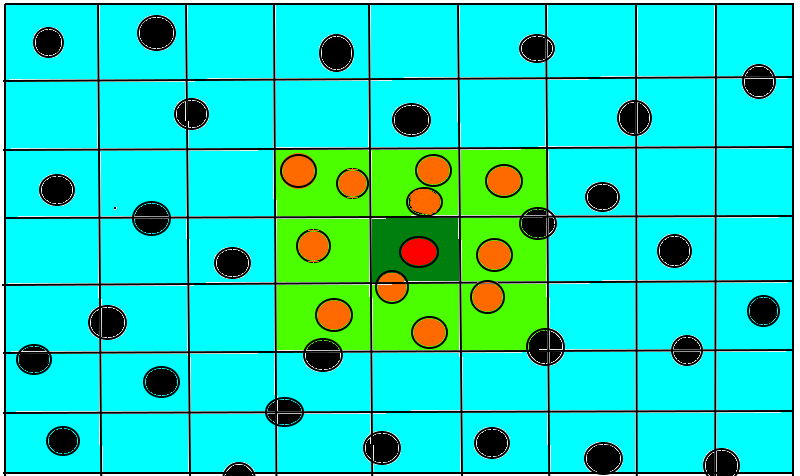
\includegraphics[width=0.5\textwidth]{chapitres/chapitre_4/figures/schematic_cell-linked_list.png}
        \caption{Schéma 2D pour l'algorithme de recherche de voisin «cell-linked liste». Les particules oranges représentent les potentiels voisins de la particule noire au centre.}
        \label{fig5}    
    \end{figure}
    
A noter que dans le cadre de nos simulations, nous nous sommes limités à l'utilisation de l'algorithme par défaut \textit{"Nsquare"} pour l'étape de recherche de voisins.

\section{Parallélisation de MFiX-EXA}

Le processus de résolution des contacts est une étape très coûteuse en temps calcul pour les solveurs granulaires, notamment lorsqu'il s'agit de simulations à grandes échelles impliquant beaucoup de particules. Un des aspects mis en avant par le solveur est le parallélisme massif, dont il a fait l'objet dans une étude récente publiée dans l'article \cite{gopalakrishnan2013development} qui illustre son potentiel en terme de Calcul Haute Performance (HPC). La parallélisation du code y est détaillée et des cas-tests de vérification y sont présentés, soulignant l'efficacité du solveur sur les architectures de calcul intensif actuelles et les gains en temps de calcul obtenus sur des simulations à grandes échelles. Nous allons donc présenter dans ce qui suit les principaux éléments de la parallélisation implémentée dans MFiX, éléments qui vont nous servir de base pour y implémenter l'approche NSCD-PDAS en parallèle.

\subsection{DEM et parallélisation}\label{parallelisation_dem}

Il existe dans la littérature différentes techniques de parallélisation de solveurs DEM. La plupart d'entre elles utilise la méthode de décomposition par domaines non seulement pour la partie fluide mais également pour la partie DEM qui, en plus de la méthode de décomposition par domaines \cite{plimpton1995fast,kavcianauskas2010parallel}, a connu d'autres techniques comme la méthode "mirror domain" \cite{darmana2006parallelization,washington2003micro}, dont le principe consiste à répartir sur chaque processeur un ensemble de données identique, on dit alors que les données sont mises en miroir par tous les processeurs. Une autre méthode appelée "particle-subset" \cite{kafui2011parallelization,plimpton1995fast} repose sur une répartition dynamique des particules et un équilibrage de charge entre tous les processeurs, de façon à affecter les particules les plus proches et en contact à un seul processeur, ce qui permet de réduire les contacts entre particules de processeurs voisins.\\

MFiX propose une technique de parallélisation basée sur la décomposition de domaine géométrique, explicitée dans l'article \cite{gopalakrishnan2013development}. Cette technique s'adapte facilement aux architectures à mémoires distribuées puisqu'elle permet d'interconnecter le réseau de sous-domaines, le parallélisme s'effectuant par échanges de données des particules (positions, vitesses, masse, rayon, densité volumique, ...). Elle permet également d'accélérer le calcul puisque le travail est réparti sur chaque sous-domaine où le nombre de particules est considérablement réduit par rapport au domaine de calcul initial (voir Figure \ref{fig7}). Néanmoins, on notera que l'équilibrage de charge pour une décomposition de domaine est effectif lorsque la distribution des particules sur les sous-domaines de calcul est uniforme.

\begin{figure}[!h]
        \centering
        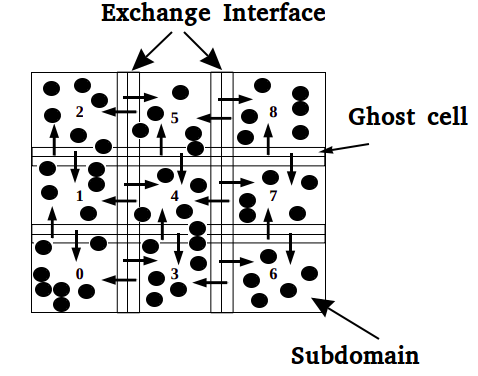
\includegraphics[width=0.6\textwidth]{chapitres/chapitre_4/figures/decomposition-echanges.png}
        \caption{Schéma simplifié des échanges de données entre sous-domaines de calcul.}
        \label{fig7}    
    \end{figure}

Chaque processeur attribué à un sous-domaine par décomposition géométrique détient des informations sur les particules qui s'y trouvent physiquement et exécute ses instructions indépendamment des autres processeurs. Le processus de communication parallèle via l'appel à des procédures de la bibliothèque MPI (Message Passing Interface) se fait par échange de données des particules se trouvant aux interfaces d'échange, constituées des cellules dites "Ghost", qui représentent la couche de cellule qui duplique les informations du processeur adjacent. Des particules dites "Ghost" permettent alors d'échanger ces informations. Une étape de synchronisation avec les particules voisines des cellules Ghost est alors nécessaire avant d'exécuter les instructions sur chacun des processeurs.  Si l'on considère par exemple à un instant $t$ une particule se trouvant à proximité d'une interface d'échange, le processeur de destination attribué au sous-domaine adjacent crée son image en particule Ghost, en dupliquant toutes ses informations. Une fois que cette particule a traversé l'interface, elle n'existe plus physiquement dans le sous-domaine initial, et le processeur attribué au sous-domaine initial va créer une particule Ghost en lieu et place de la particule initiale.\\

Enfin, d'un point de vue algorithmique, le solveur MFiX-DEM exécute à chaque pas de temps les différentes tâches impliquées dans la résolution des forces de contacts. Ensuite, les particules dont les positions et les vitesses ont été mises à jour, sont fixées sur la grille cartésienne du domaine de calcul, et les communications parallèles peuvent avoir lieu, comme décrit dans la Figure \ref{fig8}. De ce fait, les particules se déplaçant à travers les limites des processeurs sont identifiées, puis leurs données sont chargées afin de les communiquer aux processeurs de destination suivant le schéma de communication spécifique à MFiX. Les communications des données des particules se trouvant dans les cellules dites "Ghost" sont également effectuées de la même manière que celles des particules se déplaçant à travers les limites des processeurs. 

\begin{figure}[!h]
        \centering
        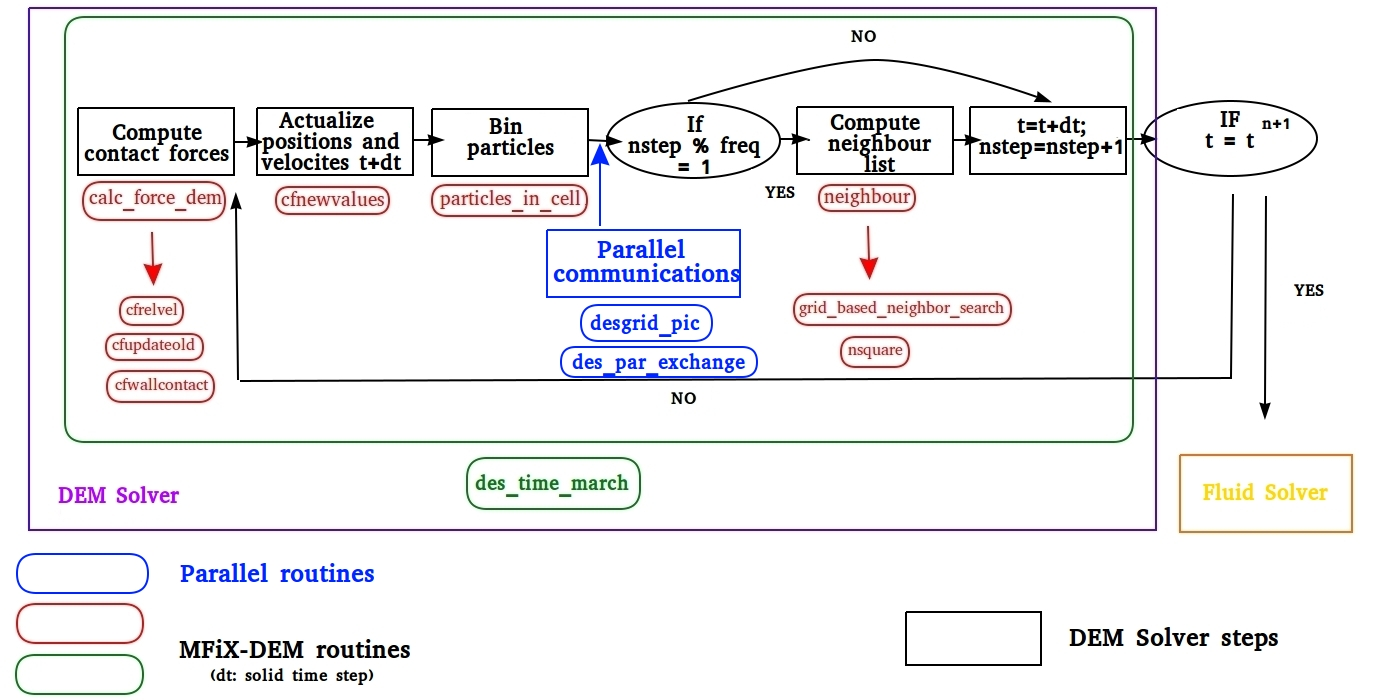
\includegraphics[width=1.0\textwidth]{chapitres/chapitre_4/figures/parallel_dem_solver_scheme.jpg}
        \caption{Organigramme d'exécution du solveur MFiX-DEM en parallèle.}
        \label{fig8}    
    \end{figure}

\subsection{Une parallélisation distribuée de la NSCD-PDAS }

On se propose dans cette partie de paralléliser la méthode NSCD-PDAS dans l'environnement de développement MFiX-EXA. On rappelle d'après la section précédente que les contraintes d'implémentation sont fortes car on est limité à une décomposition de domaine statique et géométrique. Toutefois, d'un point de vue algorithmique, on utilise le schéma de communication utilisé par la DEM.

\subsubsection{NSCD et paradigme de décomposition de domaine}

La parallélisation de la méthode NSCD par décomposition de domaine statique et géométrique reste une tâche difficile à mettre en oeuvre du fait de la non-régularité des interactions de contact en milieu multi-corps rigides et de la non-unicité de la solution de ce genre de problèmes. Dans ce sens, plusieurs stratégies ont été proposées dans la littérature pour introduire ces techniques dans le cadre de la NSCD. Celles-ci peuvent être catégorisées selon deux familles; à savoir la méthode sans chevauchement FETI-LIKE DDM (Finite Element Tearing and Interconnecting Domain Decomposition Method), proposée dans \cite{alart2012nonlinear} qui consiste à introduire un problème d'interface linéaire en répartissant les interactions de contact dans les différents sous-domaines, et la méthode avec chevauchement minimal de type Schwarz (SCHWARZ-LIKE DDM) dont les développements théoriques et numériques 
ont été étudiés dans \cite{visseq2013high}. D'ailleurs, les principaux travaux de développement de la plateforme du LMGC90 (Logiciel de Mécanique Gérant le Contact) ont porté sur l'implémentation et l'enrichissement de ces deux familles de décomposition de domaine. On notera que le choix de répartition des interactions de contact parmi les sous-domaines dans les techniques de décomposition pré-citées a été motivé par leur caractère non-régulier, selon un partitionnement dit "dual" décrit dans \cite{visseq2013high}.\\
Un autre partitionnement dit "primal", consiste quant à lui à distribuer non pas les interactions mais les particules dans les sous-domaines, avec une interface définie par l'ensemble des interactions non-régulières pour faire le lien entre les particules de deux sous-domaines adjacents.


\subsubsection{Algorithme parallèle de résolution}

Pour mettre en oeuvre la parallélisation de la NSCD dans le cadre de MFiX et réaliser l'ensemble des cas-tests, nous nous sommes basés sur l'algorithme parallèle pour la DEM utilisant le paradigme de décomposition de domaine statique. Notre point de départ est la recherche de voisins qui permet d'établir la liste des contacts sur l'ensemble du domaine de calcul décomposé, en tenant compte de l'emplacement des particules à un instant $t$ donné. Comme indiqué à la section \ref{parallelisation_dem}, chaque processeur détient non seulement les informations des particules appartenant au sous-domaine attribué, mais également celles des particules se trouvant dans les cellules ghost qui dupliquent les informations des processeurs adjacents. On peut d'ailleurs mettre en lien cette approche avec la technique de partitionnement primal, puisque la répartition est effectuée sur la base des particules et non des interactions.\\

Nous avons ainsi exploité le processus d'échange de données s'effectuant au niveau des cellules ghost pour distinguer deux types de contacts; ceux entre particules Normales dont l'emplacement physique est à l'intérieur du processeur, puis ceux impliquant une particule d'interface et une particule Ghost. À chaque itération temporelle, nous traitons une distribution de particules Normales et Ghosts (voir Figure \ref{normal_ghost_scheme}), et la résolution de la loi de contact et de frottement est réalisée par sous-domaine à l’aide du même algorithme utilisé dans le cas mono-domaine, en itérant de façon non-linéaire sur l'ensemble des contacts de chaque système restreint.

\begin{figure}[!h]
  \centering
    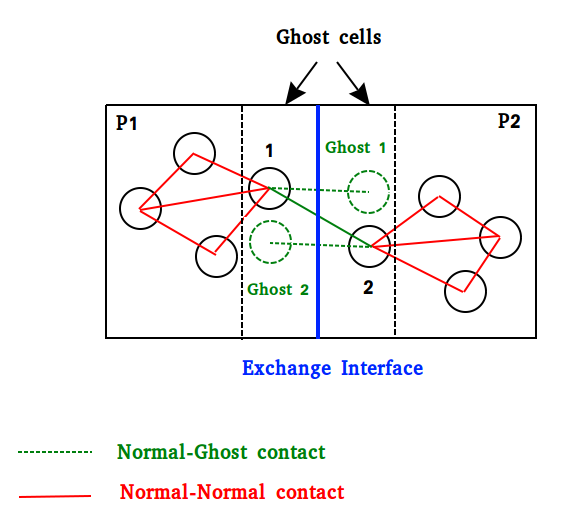
\includegraphics[width=0.6\textwidth]{chapitres/chapitre_4/figures/normal_ghost_scheme.png}
    \caption{\centering Schéma de communication entre deux processeurs dans le cadre de la parallélisation de la NSCD.}\label{normal_ghost_scheme}
\end{figure}

Après une synchronisation des données des cellules ghost, le solveur non-linéaire NLGS itère sur l'ensemble des contacts "Normale-Ghost" ($\alpha_{N-G}$) afin de mettre à jour ces contacts de frontière. Les données des particules "Normales" d'interface sont actualisées et communiquées au processeur adjacent. Une fois que les contacts "Normale-Ghost" sont traités, le solveur NLGS itère sur l'ensemble des contacts n'impliquant que des particules "Normales" du même sous-domaine pour y résoudre la loi de contact et mettre à jour leurs données. Par une synchronisation MPI, ces données sont ensuite propagées au niveau des cellules ghost, puis communiquées au processeur adjacent. Ce schéma de communication s'apparente à un schéma hybride de Gauss Seidel/Jacobi par bloc.\\

\begin{algorithm}[H]
  \SetAlgoLined
  \KwData{positions des particules}
  \KwResult{Résolution des contacts en parallèle}
 
  Création des particules Ghost\;
  Détection des contacts et construction de la liste des voisins\;
  \For{$j\leftarrow 0$ \KwTo $N_{NLGS}$, (jusqu'à convergence)}{
    Synchronisation des cellules ghost\;
    \For{$\alpha \leftarrow 1$ \KwTo $N_{\alpha}$ (boucle sur les contacts)}{
        \If{$\alpha == \alpha_{N-G}$}{
        Calcul de la loi de contact et frottement (PDAS)\;
        Actualisation vitesses globales $P_{N-N}$\;
        }
    }
    \For{$\alpha \leftarrow 1$ \KwTo $N_{\alpha}$ (boucle sur les contacts)}{
        \If{$\alpha \neq \alpha_{N-G}$}{
        Calcul de la loi de contact et frottement (PDAS)\;
        Actualisation vitesses globales par bloc\;
        }
    }
    Synchronisation des cellules ghost\;
	Communication et échange de données via les cellules ghost\;
    }
  Actualisation des déplacements généralisés par bloc\;
  \caption{Algorithme parallèle MFiX-NSCD-PDAS.}
\end{algorithm}

\section{Comparaisons DEM-CUNDALL / NSCD-PDAS}

Plusieurs études comparatives entre les approches DEM-CUNDALL et NSCD-PDAS sont proposées dans cette section. Ceci est rendue possible en utilisant le modèle de CUNDALL implémenté dans MFiX-EXA. Les premières comparaisons sont réalisées sur des configurations impliquant une seule particule afin de valider la bonne implémentation des lois de contact et de frottement. Enfin, une étude comparative est munie pour l'écoulement de grains dans un tambour rotatif.

\subsection{Éléments de comparaison sur une particule}

\subsubsection{Rebond d'une particule}

Dans ce paragraphe, on se propose de comparer les schémas numériques DEM et NSCD dans le cas d'une particule P qui rebondit sur une fondation rigide. Il s'agit de comparer le modèle de contact non-régulier NSCD et de souligner les propriétés du modèle de Cundall dans le cas d'un rebond pour lequel on connaît la solution analytique. Pour cela, nous considérons une particule rigide P, lâchée sans vitesse initiale ($v_0 = 0$), d'une hauteur initiale $h_0$, soumise uniquement à la force de gravité $\vect{g}$. Les paramètres physiques relatifs au cas-test sont répertoriés dans la Table ci-dessous:

\begin{center}
\begin{table}[!h]
\begin{tabular}{ |p{6.2cm}|p{6.2cm}| }
 \hline \rowcolor{lightgray}
 Paramètre& Valeur\\
 \hline
 Rayon particule P  ($m$) & $r_p = 4\times10^{-3}$\\
 Densité volumique ($Kg.m^{-3}$)& $\rho = 2700$\\
 Hauteur initiale ($m$) & $h_0 = 0.225$\\
 Vitesse initiale  ($m.s^{-1}$)  &$v_0 = 0$\\
 Force de gravité ($m.s^{-2}$)& $g = -9.80665$\\
 Masse de la particule ($Kg$)  &$m_p = \rho \pi r_p^{2}$\\
 \hline
\end{tabular}
\caption{Paramètres physiques pour la simulation de chute d'une particule.}\label{tab_41}
\end{table}
\end{center}
\vspace{-1cm}
\noindent Pour l'approche de CUNDALL, les paramètres numérique du modèle physique sont répertoriés dans la Table \ref{tab_42}. On notera que pour l'approche NSCD-PDAS, seuls les paramètres $e_n$, $e_t$, $\gamma_n$, $\gamma_t$ et $\epsilon_{NLGS}$ sont à définir. On rappelle que $k_n$ (resp. $k_t$) est la constante de raideur normale (resp. tangentielle) de contact, $\eta_{ratio}$ le ratio entre le coefficient d'amortissement normal et tangentiel, $\gamma_n$ (resp. $\gamma_t$) est le paramètre active set normal (resp. tangentiel), et $\epsilon_{NLGS}$ le critère d'arrêt de la méthode numérique PDAS.

\begin{center}
\begin{table}[!h]
\begin{tabular}{ |p{5.5cm}|p{3.8cm}|p{3.4cm}| }
 \hline \rowcolor{lightgray}
 DEM-CUNDALL& NSCD-PDAS& Communs\\
 \hline
 $e_n = 0.59$ & $e_n = 0.46$ & $T = 2 \quad s$\\
 -& $e_t = 1$ & -\\
 $k_n = (10^4, 10^5, 10^6) \quad N.m^{-1}$ & $\gamma_n = 0.1$ & $\mu = 0$\\
 $k_t = \frac{2}{7} k_n \quad N.m^{-1}$ & $\gamma_t = 0.1$ & -\\
 $\eta_{ratio} = 0.5$& $\epsilon_{NLGS} =  10^{-8}$ & -\\
 $dt \approx (12.3, 3.89, 1.23) \times 10^{-6}$ s & $dt = 5\times10^{-5}$ \quad s& -\\
 \hline
\end{tabular}
\caption{Paramètres numériques pour la simulation de chute d'une particule pour chaque approche de contact.}\label{tab_42}
\end{table}
\end{center}
\vspace{-1cm}
Un paramètre important du modèle de CUNDALL explicite est le temps de collision. Ce dernier caractérise le temps de contact entre deux particules, un temps de contact élevé est associé à des particules rigides, et à l'opposé, un temps de collision infiniment petit correspond à un contact entre deux particules déformables. La constante de raideur $k_n$ conditionne ce point clé du modèle, par la relation:

\vspace{-0.5cm}
\begin{equation}
    t_{coll} = \pi \Bigg[\frac{k_n}{m_{eff}} - (\frac{\eta_n}{2m_{eff}})^2\Bigg]^{-1/2}\label{t_coll}
\end{equation}

\noindent où $m_{eff}$ représente la masse effective de la collision entre la particule et la fondation rigide, et $\eta_n$ le coefficient d'amortissement visqueux normal. On notera également que le coefficient de restitution normal $e_n$ relatif à l'approche NSCD-PDAS est différent de celui utilisé pour la DEM. En effet, ce dernier a été ajusté de façon empirique pour obtenir un $e_n$ effectif (voir Figure \ref{fig74}). Le coefficient de restitution normal effectif ainsi obtenu est de $0.46$.

\begin{figure}[!h]
  \centering
    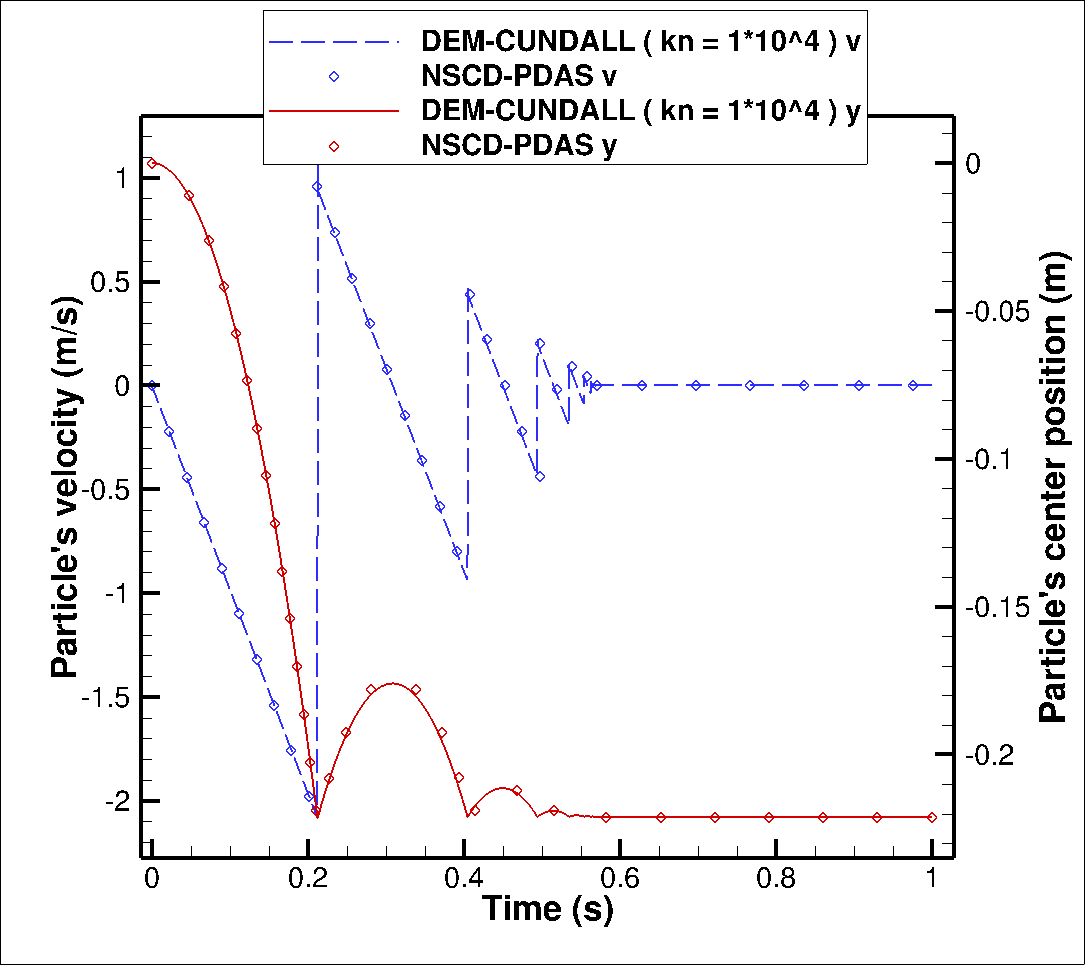
\includegraphics[width=0.5\textwidth]{chapitres/chapitre_4/figures/vel-pos-y_chute-libre.png}
    \caption{\centering Positions et vitesses de la particule en chute libre au cours du temps obtenues par DEM-CUNDALL et NSCD-PDAS.}\label{fig74}
\end{figure}

Pour le modèle DEM-CUNDALL, le pas de temps varie selon la relation \ref{t_coll}. Pour le modèle NSCD-PDAS, le pas de temps est pris plus grand ($dt_{NSCD}>dt_{DEM}$). Le comportement de la particule lors du processus de chute libre est identique pour les deux approches. En l'absence de frottement, et pour un coefficient de restitution normal $e_n = 0.46$, le mouvement de la particule devient statique au bout de quelques rebonds. De plus, d'après les graphes de la Figure \ref{fig74}, la variation numérique de la position de la particule au cours du temps obtenue par NSCD-PDAS (symbole $\circ$ en rouge) correspond à celle obtenue par DEM-CUNDALL. De même, la solution numérique de la vitesse de la particule au cours du temps obtenue par NSCD-PDAS (symbole $\circ$ en bleu) varie de la même manière que la solution numérique obtenue par DEM-CUNDALL. Le comportement de la solution numérique est donc identique pour les deux approches.\\

L'autre propriété pertinente à comparer est l'énergie cinétique de la particule. Pour l'approche DEM-CUNDALL, la variation du constante de raideur normale de contact $k_n$ permet d'étudier le comportement local de la particule. Ce paramètre devant être choisi suffisamment élevé pour que la distance d'interpénétration reste faible par rapport au diamètre de la particule au moment du choc, nous avons pris 3 valeurs pour la constante de raideur normale ($k_n = 10^4, 10^5, 10^6$) pour comparer les solutions obtenues à celles de l'approche NSCD-PDAS. D'après les graphes de la Figure \ref{fig84}, il apparaît clairement que l'influence de la constante de raideur normale $k_n$ sur le comportement de la particule au moment du choc est notable et cela se traduit par une variation de l'énergie cinétique au cours du temps légèrement différente selon le $k_n$ choisi. Ainsi, plus le $k_n$ est grand, plus on tend vers la solution numérique obtenue par NSCD-PDAS (symbole $\bullet$ en rouge), et plus petit est le pas de temps.

\begin{figure}[h!]
   \subfloat[\label{ec_chute}]{%
      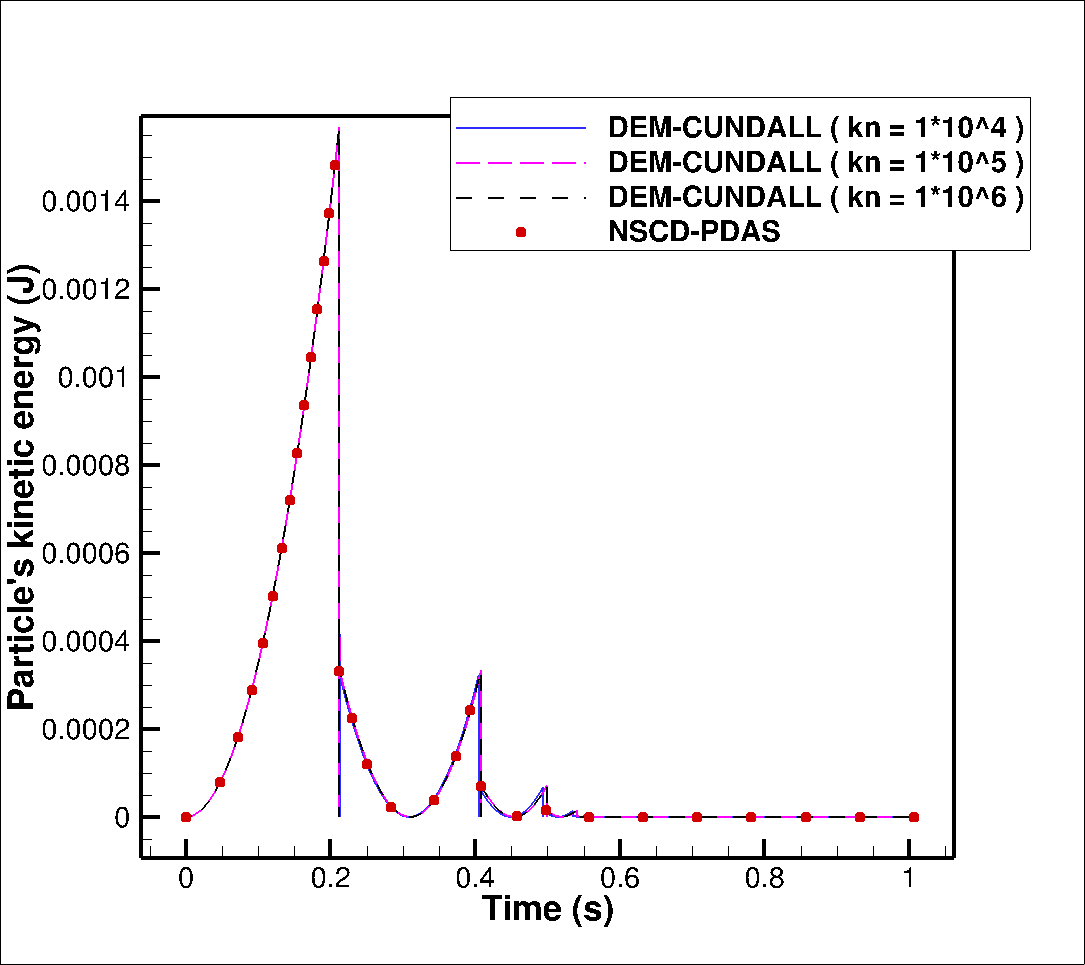
\includegraphics[width=0.5\textwidth]{chapitres/chapitre_4/figures/ec_chute_libre.png}}
\hspace{\fill}
   \subfloat[\label{ec_chute_zoom}]{%
      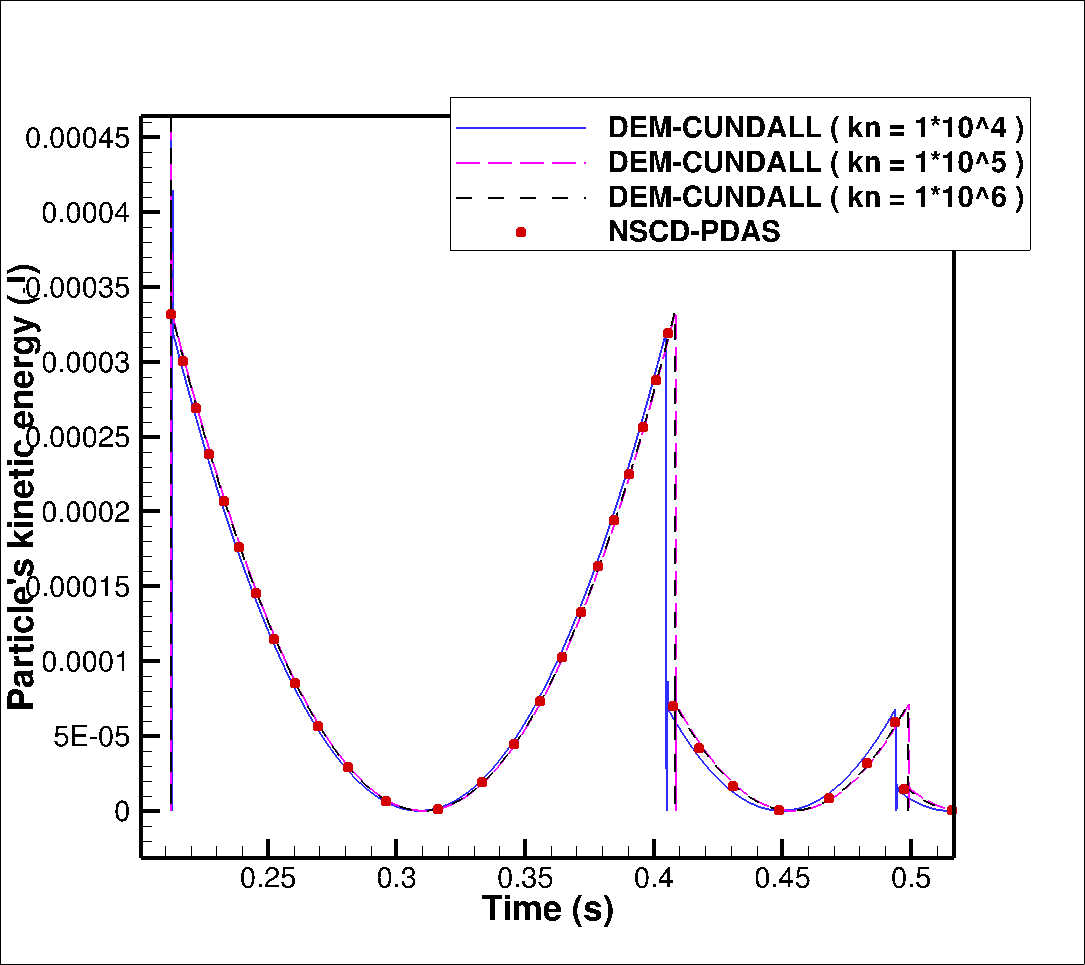
\includegraphics[width=0.5\textwidth]{chapitres/chapitre_4/figures/ec_chute_libre_zoom.png}}\\
\caption{\centering Variations de l'énergie cinétique de la particule en chute libre au cours du temps obtenues par DEM-CUNDALL (pour différentes constantes de raideur normale $k_n$) et NSCD-PDAS.}\label{fig84}
\end{figure}

\subsubsection{Roulement-glissement dans un tambour rotatif}

Nous poursuivons notre étude comparative entre l'approche DEM-CUNDALL et l'approche NSCD-PDAS par un second cas-test de roulement-glissement dans un tambour rotatif. Une particule, de rayon $4\times10^{-3}$ m, posée sans vitesse initiale au fond d'un tambour tournant à une vitesse de rotation de $6$ rpm dans le sens anti-horaire, est soumise à l'action de la rotation du tambour. Il s'agit alors d'étudier le mouvement de la particule dans le tambour et de comparer le comportement des solutions numériques obtenues par DEM-CUNDALL et NSCD-PDAS. Les paramètres physiques relatifs à la simulation sont donnés dans la Table ci-dessous:

\begin{center}
\begin{table}[!h]
\begin{tabular}{ |p{6.5cm}|p{6.1cm}| }
 \hline \rowcolor{lightgray}
 Paramètre& Valeur\\
 \hline
 Rayon particule P  ($m$) & $r_p = 4\times10^{-3}$\\
 Densité volumique ($Kg.m^{-3}$)& $\rho = 2700$\\
 Diamètre du tambour ($mm$) & $D_{drum} = 450$\\
 Vitesse de rotation du tambour ($rpm$) & $\Omega_{drum} = 6$\\
 Vitesse initiale  ($m.s^{-1}$)  &$v_0 = 0$\\
 Force de gravité ($m.s^{-2}$)& $g = -9.80665$\\
 Masse de la particule ($Kg$)  &$m_p = \rho \pi r_p^{2}$\\
 \hline
\end{tabular}
\caption{Paramètres physiques pour la simulation de roulement-glissement dans un tambour rotatif.}\label{tab_43}
\end{table}
\end{center}

\vspace{-1.5cm}

\noindent Les paramètres numériques sont reportés dans la Table \ref{tab_44} selon l'approche utilisée. 

\begin{center}
\begin{table}[!h]
\begin{tabular}{ |p{5.5cm}|p{3.8cm}|p{3.4cm}| }
 \hline \rowcolor{lightgray}
 DEM-CUNDALL& NSCD-PDAS& Communs\\
 \hline
 $dt \approx 1.23\times10^{-5} \quad s$ & $dt = 5\times10^{-5} \quad s$ & $T = 2 \quad s$\\
 $k_n = 10^4 \quad N.m^{-1}$ & $\gamma_n = 10^{-8}$ & -\\
 $k_t = \frac{2}{7} k_n \quad N.m^{-1}$ & $\gamma_t = 10^{-8}$ & $\mu = 0.2$\\
 $\eta_{ratio} = 0.5$ & $\epsilon_{NLGS} =  10^{-8}$ & -\\
 \hline
\end{tabular}
\caption{Paramètres numériques pour la simulation de roulement-glissement dans un tambour rotatif pour chaque approche de contact.}\label{tab_44}
\end{table}
\end{center}

Initialement au repos, la particule, entraînée par la rotation du tambour, entame un mouvement oscillatoire identique à celui du pendule (voir Figure \ref{fig94}). En effet, la force de frottement entre la paroi intérieure du tambour et la particule amorce le mouvement de la particule qui roule dans la direction opposée au sens de rotation du tambour. On notera que $dt_{NSCD}>dt_{DEM}$.

\begin{figure}[!h]
  \centering
    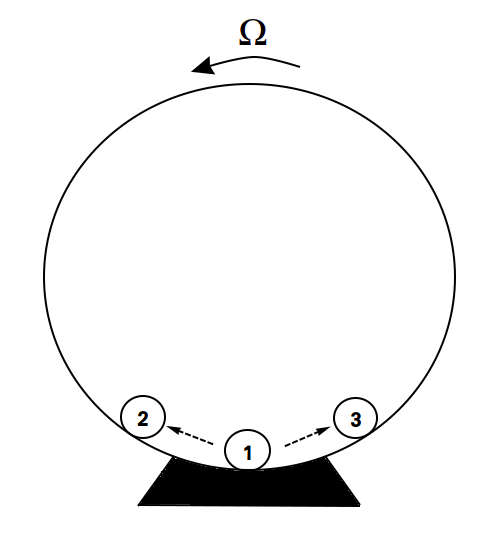
\includegraphics[width=0.3\textwidth]{chapitres/chapitre_4/figures/roulement_glissement_tambour.png}
    \caption{\centering Régime oscillatoire de la particule en roulement-glissement dans un tambour rotatif.}\label{fig94}
\end{figure}

Le graphe de la Figure \ref{fig104} décrivent d'une part l'évolution temporelle de la vitesse angulaire de la particule qui glisse et roule sous l'action de la rotation du tambour, et d'autre part l'évolution de l'énergie cinétique de cette particule. On constate alors que la solution numérique de la vitesse angulaire obtenue par NSCD-PDAS (symbole $\circ$ en bleu) varie de manière identique à celle obtenue par DEM-CUNDALL. Il en est de même pour la solution numérique de l'énergie cinétique (courbe rouge et symbole $\circ$ en rouge).

\begin{figure}[!h]
  \centering
    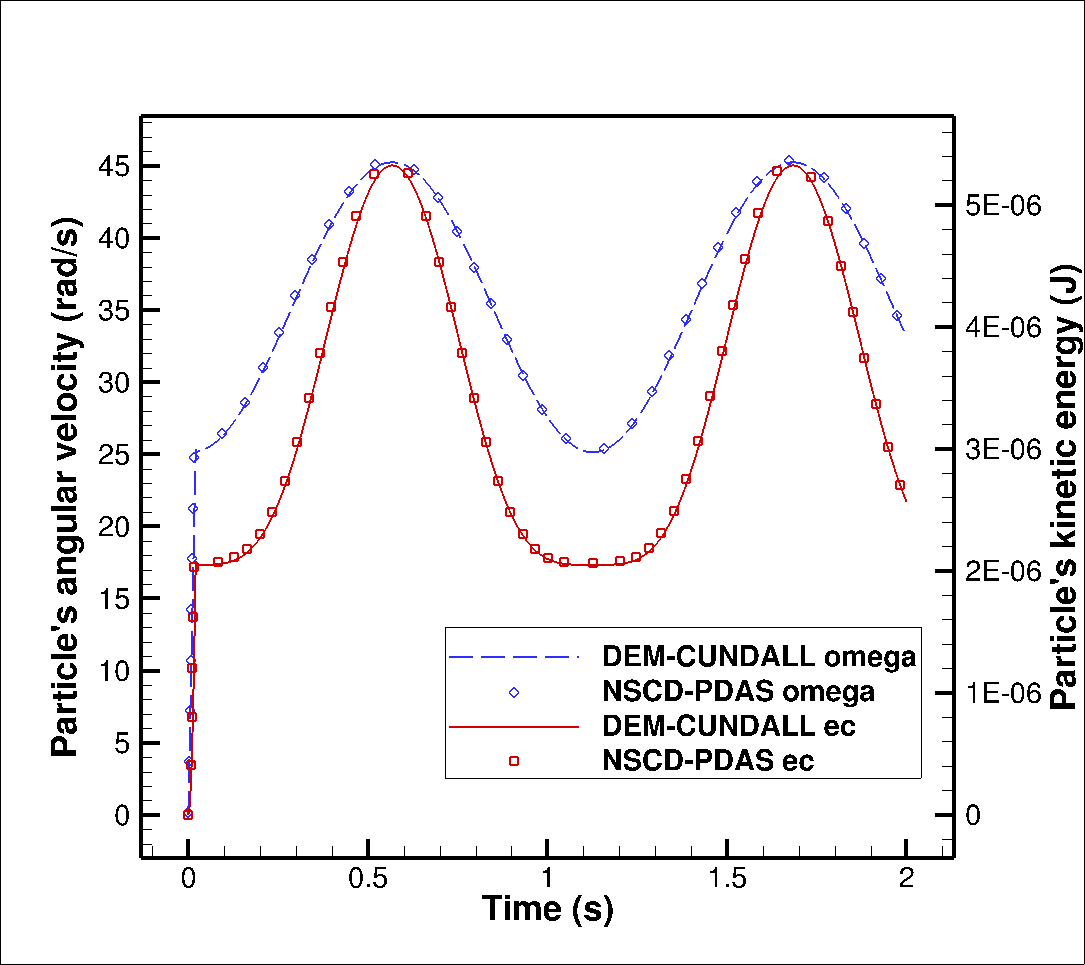
\includegraphics[width=0.55\textwidth]{chapitres/chapitre_4/figures/ec-omega_roll-slide.png}
    \caption{\centering Variations de la vitesse angulaire (en bleu) et de l'énergie cinétique ( en rouge) de la particule en roulement-glissement au cours du temps obtenues par DEM-CUNDALL et NSCD-PDAS.}\label{fig104}
\end{figure}

Les cas-tests réalisés sur les configurations mono-particules indiquent une concordance entre les modèles DEM et NSCD. Compte tenu de l'utilisation antérieure importante de la DEM implémentée dans MFiX-EXA, cela constitue un élément complémentaire de la méthode NSCD. De plus, le caractère implicite de la méthode NSCD offre une stabilité numérique temporelle supérieure. En effet, la prise en compte de particules rigides avec le modèle DEM-CUNDALL se traduit par des pas de temps infiniment petits.


\subsection{Écoulement granulaire dans un tambour rotatif}

Le but de cette section est de poursuivre notre étude comparative DEM-CUNDALL / NSCD-PDAS en considérant un écoulement granulaire à travers une simulation de particules confinées dans un tambour rotatif. Pour cette étude, nous simulons une collection de $400$ particules de diamètres uniformément distribués entre $7$ et $8$ mm déposées au fond d'un tambour de diamètre $450$ mm et de vitesse de rotation égale à $6$ rpm. Le choix d'une distribution aléatoire uniforme a été motivé par le phénomène de "cristallisation" ou "blocage" visible lorsque les particules simulées sont de tailles identiques. La distribution aléatoire uniforme ainsi choisie permet d'éviter ces blocages au cours du processus de rotation. Les particules s'organisent alors en deux couches, une en contact avec la paroi interne du tambour et l'autre sous forme de lit. Pour ce cas-test, les simulations ont été réalisé en parallèle en utilisant $96$ processeurs. Nous allons évaluer dans un premier temps l'inclinaison de la surface libre par DEM-CUNDALL et NSCD-PDAS en régime établi. Pour cela, nous simulons sur un temps d'intégration de $5$ secondes. Les paramètres physiques et numériques sont reportés ci-dessous:

\begin{center}
\begin{table}[!h]
\begin{tabular}{ |p{6.5cm}|p{6.1cm}| }
 \hline \rowcolor{lightgray}
 Paramètre& Valeur\\
 \hline
 Rayons particules  ($mm$) & $r = [3.5 - 4]$\\
 Densité volumique ($Kg.m^{-3}$)& $\rho = 2700$\\
 Diamètre du tambour ($mm$) & $D_{drum} = 450$\\
 Vitesse de rotation du tambour ($rpm$) & $\Omega_{drum} = 6$\\
 Vitesse initiale  ($m.s^{-1}$)  &$v_0 = 0$\\
 Force de gravité ($m.s^{-2}$)& $g = -9.80665$\\
 Masse de la particule ($Kg$)  &$m_p = \rho \pi r_p^{2}$\\
 \hline
\end{tabular}
\caption{Paramètres physiques pour la simulation d'un écoulement granulaire dans un tambour rotatif.}\label{tab_45}
\end{table}
\end{center}

\vspace{-1cm}

\begin{center}
\begin{table}[!h]
\begin{tabular}{ |p{5cm}|p{3.8cm}|p{3.4cm}| }
 \hline \rowcolor{lightgray}
 DEM-CUNDALL& NSCD-PDAS& Communs\\
 \hline
 $e_n = 0.59$ & $e_n = 0.46$ & $T = 5 \quad s$\\
 $k_n = 10^3 \quad N.m^{-1}$& $e_t = 1$ & -\\
 $k_t = \frac{2}{7} k_n \quad N.m^{-1}$ & $\gamma_n = 10^{-8}$ & $\mu = 0.2$\\
 $\eta_{ratio} = 0.5$ & $\gamma_t = 10^{-8}$ & -\\
 - & $\epsilon_{NLGS} =  10^{-8}$ & -\\
 $dt \approx 3.8\times10^{-6} \quad s$ &$dt = 1\times10^{-5} \quad s$ &-\\
 \hline
\end{tabular}
\caption{Paramètres numériques pour la simulation d'un écoulement granulaire dans un tambour rotatif pour chaque approche de contact.}\label{tab_46}
\end{table}
\end{center}

\vspace{-1cm}

La Figure \ref{tambour_400} montre que l'écoulement atteint un régime établi après $5$ secondes de simulation et qu'il est quasiment identique pour les deux approches en parallèle, avec $dt_{NSCD}>dt_{DEM}$.

\begin{figure*}[h!]
   \subfloat[\label{tambour_400_dem_diam}]{%
      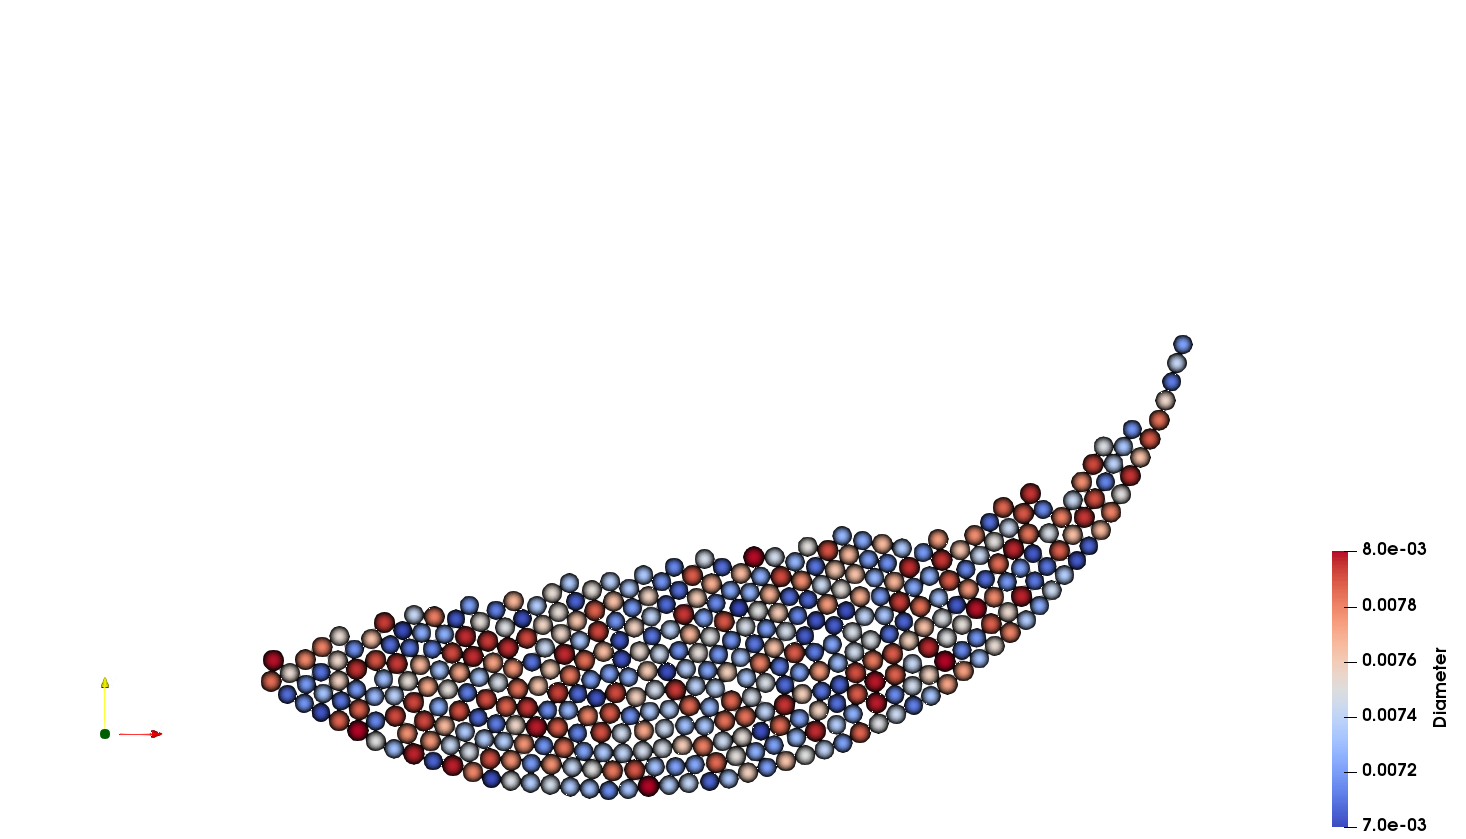
\includegraphics[trim=100 20 10 60,clip, width=0.5\textwidth]{chapitres/chapitre_4/figures/DEM_tambour-400_diameter.png}}
\hspace{\fill}
   \subfloat[\label{tambour_400_dem_rank}]{%
      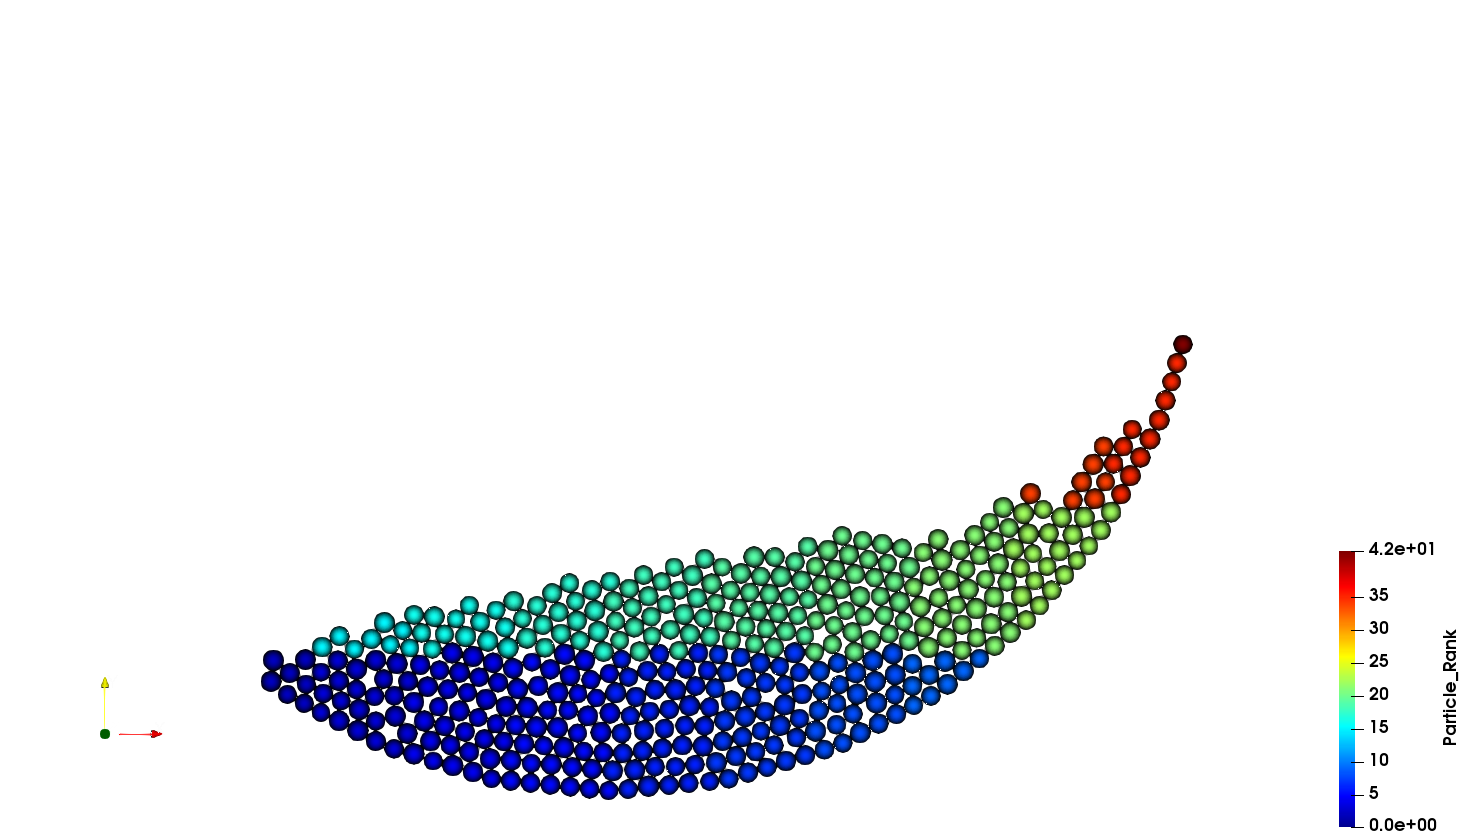
\includegraphics[trim=100 20 10 60,clip, width=0.5\textwidth]{chapitres/chapitre_4/figures/DEM_tambour-400_rank.png}}\\
\hspace{\fill}
   \subfloat[\label{tambour_400_nscd_diam}]{%
      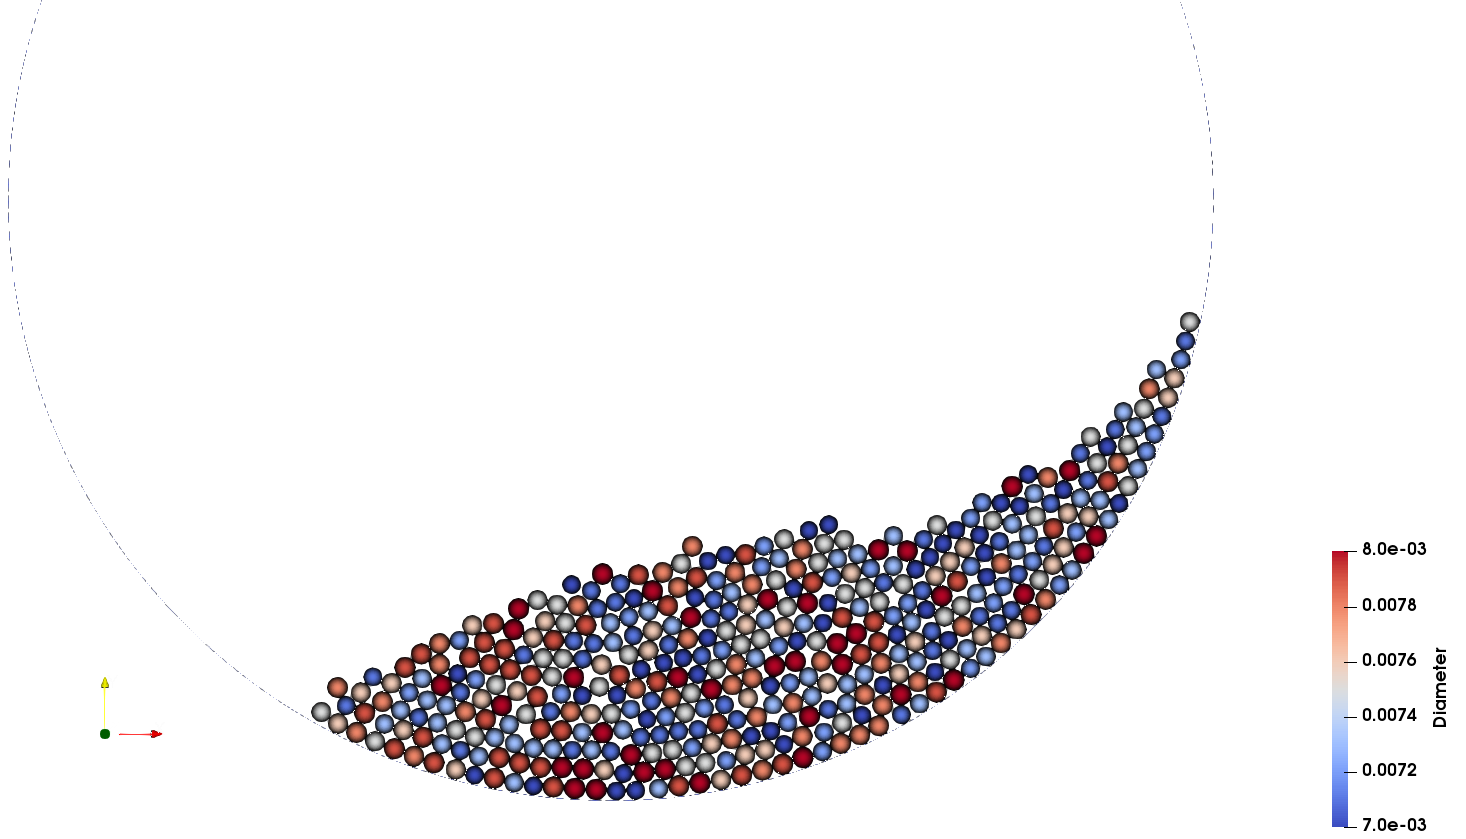
\includegraphics[trim=100 20 10 60,clip, width=0.5\textwidth]{chapitres/chapitre_4/figures/NSCD_tambour-400_diameter.png}}
\hspace{\fill}
   \subfloat[\label{tambour_400_nscd_rank}]{%
      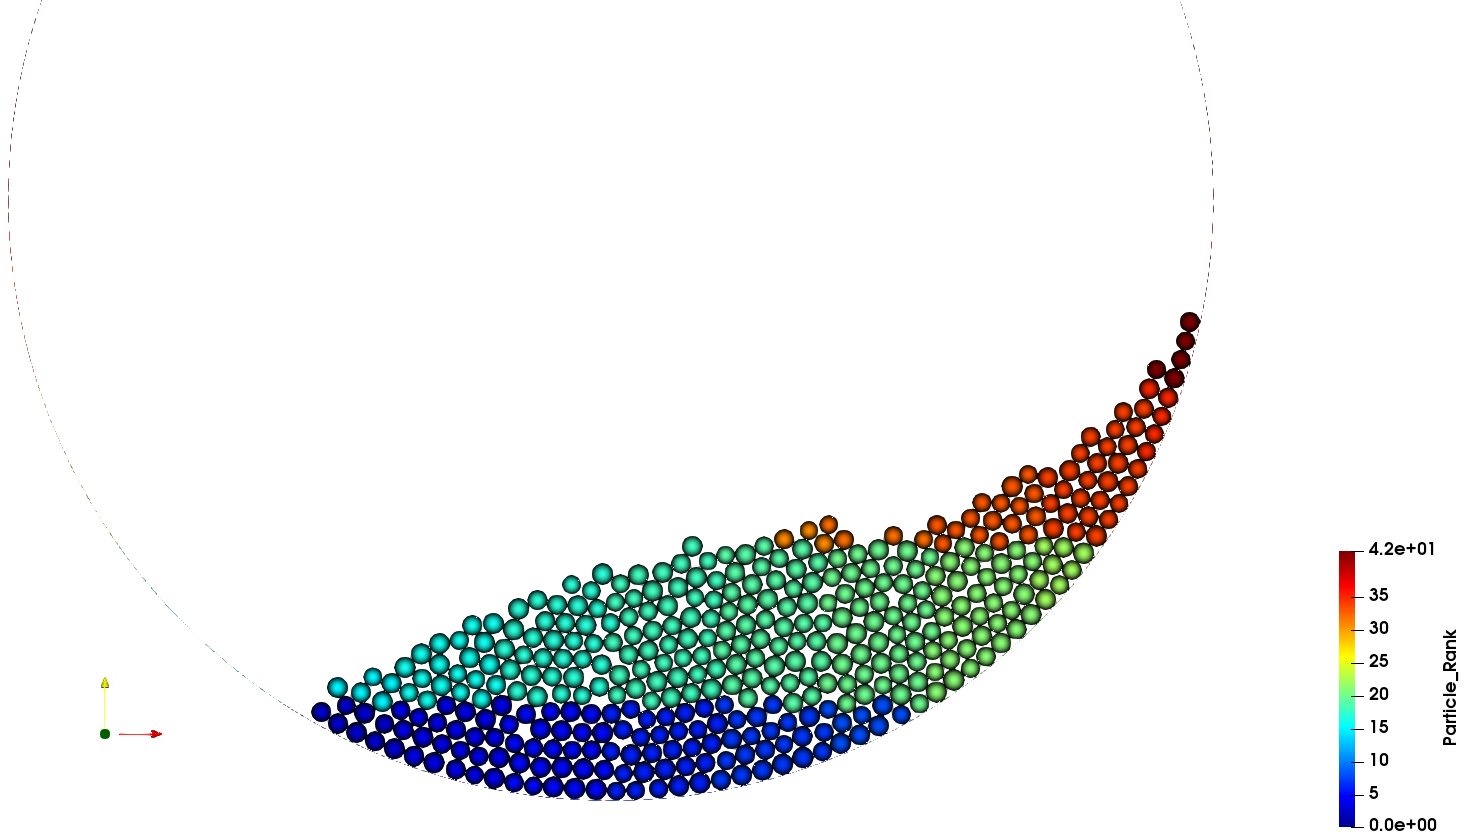
\includegraphics[trim=100 20 10 60,clip, width=0.5\textwidth]{chapitres/chapitre_4/figures/NSCD_tambour-400_rank.png}}\\
\caption{\label{tambour_400}Instantanées des profils d'écoulements granulaires dans un tambour rotatif à 400 particules de distribution aléatoire obtenues par DEM-CUNDALL [(a) diamètre particules, (b) rang processeurs] et NSCD-PDAS [(c) diamètre particules, (d) rang processeurs] en régime établi.}
\end{figure*}

Le régime établi est atteint après la phase de sédimentation des particules. Celles-ci se tassent les unes sur les autres, formant ainsi un lit de particules. Lorsque l'inclinaison est constante, les particules au contact de la paroi du tambour se déplacent à une vitesse plus faible que celle qui se trouvent à la surface libre à cause du poids exercé par le lit de particules. Les impulsions normales dues à la persistance des contacts exercées sur chaque particule engendrent une interpénétration que l'on mesure pour les deux approches  DEM-CUNDALL et NSCD-PDAS. La Figure \ref{tambour_400_nscd_penetration} confirme que la formulation non-régulière des conditions de contact et de frottement résolue avec l'approche NSCD assure une non-interpénétrabilité entre les corps. En effet, on observe une pénétration moyenne de l'ordre de $10^{-7}$ mètres sur quelques contacts. Avec l'approche DEM-CUNDALL, une interpénétrabilité plus importante est observée, de l'ordre de $10^{-6}$ mètres sur une bonne partie des contacts pour une constante de raideur normale $k_n = 10^3 N.m^{-1}$, (cf. Figure \ref{tambour_400_dem_penetration}). C'est un résultat attendu puisque le modèle DEM-CUNDALL autorise l'interpénétration entre particules.

\begin{figure*}[h!]
   \subfloat[\label{tambour_400_dem_penetration}]{%
      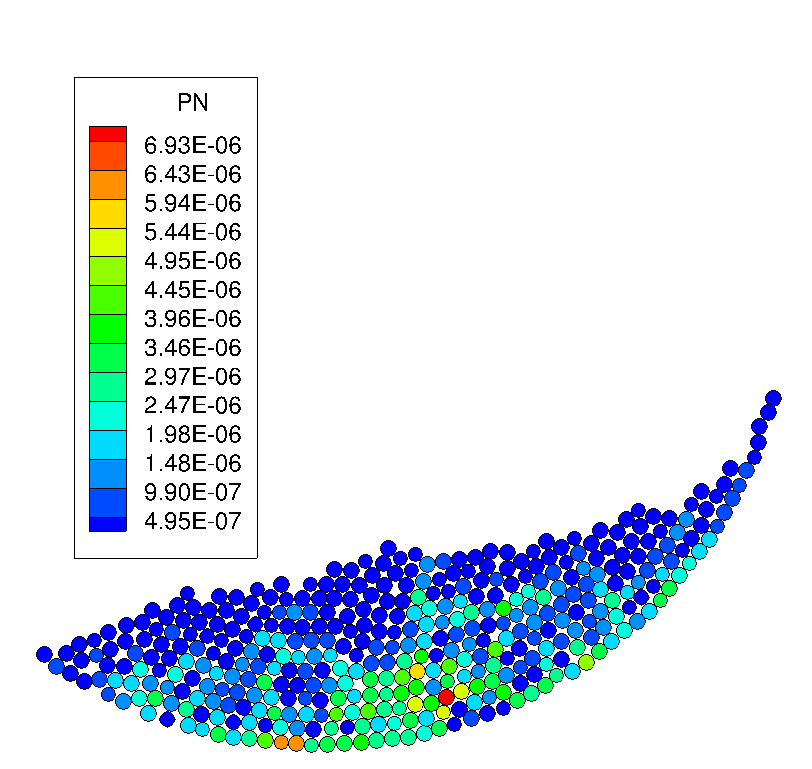
\includegraphics[trim=50 20 10 60,clip, width=0.45\textwidth]{chapitres/chapitre_4/figures/penetration_dem.png}}
\hspace{\fill}
   \subfloat[\label{tambour_400_nscd_penetration}]{%
      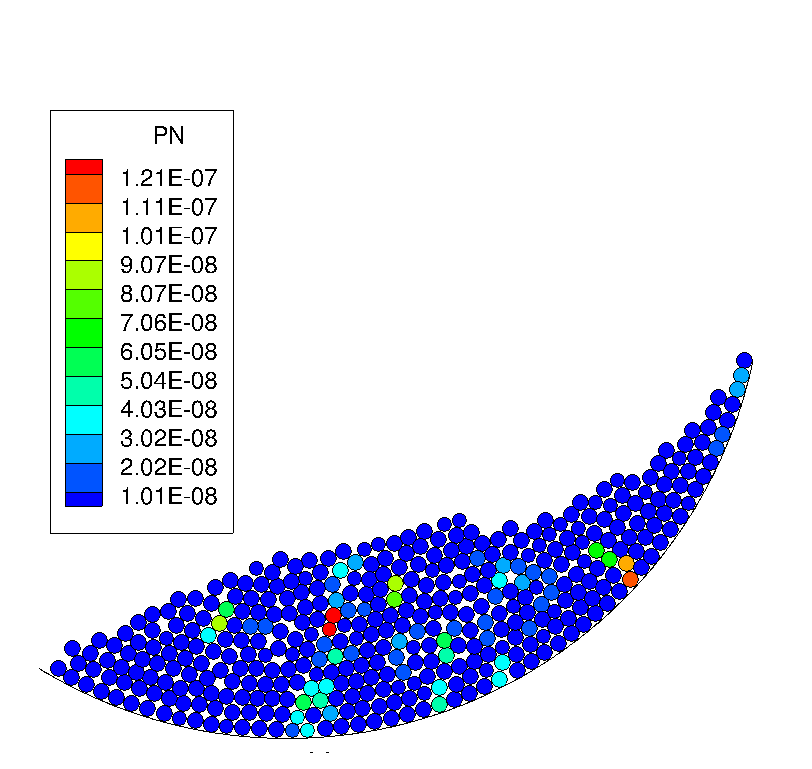
\includegraphics[trim=50 20 10 60,clip, width=0.45\textwidth]{chapitres/chapitre_4/figures/penetration_nscd.png}}\\
\caption{\label{tambour_400_penetration}Visualisation des interpénétrations lors des simulations d'écoulements granulaires dans un tambour rotatif à 400 particules de distribution aléatoire obtenues par (a) DEM-CUNDALL et (b) NSCD-PDAS à écoulement de surface régulier atteint.}
\end{figure*}

Enfin, pour mettre en avant le caractère conservatif de l'approche NSCD-PDAS, nous avons comparé l'évolution de l'énergie cinétique au cours du temps entre les deux approches, en faisant varier la constante de raideur normale pour l'approche DEM-CUNDALL. Nous observons d'après le graphe de la Figure \ref{fig134} qu'en régime établi, l'énergie cinétique possède un niveau moyen qui ne décroît pas au cours du temps avec l'approche NSCD-PDAS (courbe rouge). Les oscillations correspondent au mouvement périodique dit "avalanche" d'accumulation des particules sur le côté droit du tambour. Pour ce qui est de l'approche DEM-CUNDALL, l'influence de la constante de raideur est notable puisqu'avec un $k_n = 10^3 N.m^{-1}$, cela implique des interpénétrations plus importantes, et une forte diminution de l'énergie cinétique en régime établi, et pour un $k_n$ pris égal à $10^5  N.m^{-1}$, l'évolution de l'énergie cinétique tend approximativement vers le cas limite de la quantité d'énergie en régime établi correspondant à l'approche NSCD-PDAS.

\begin{figure}[!h]
  \centering
    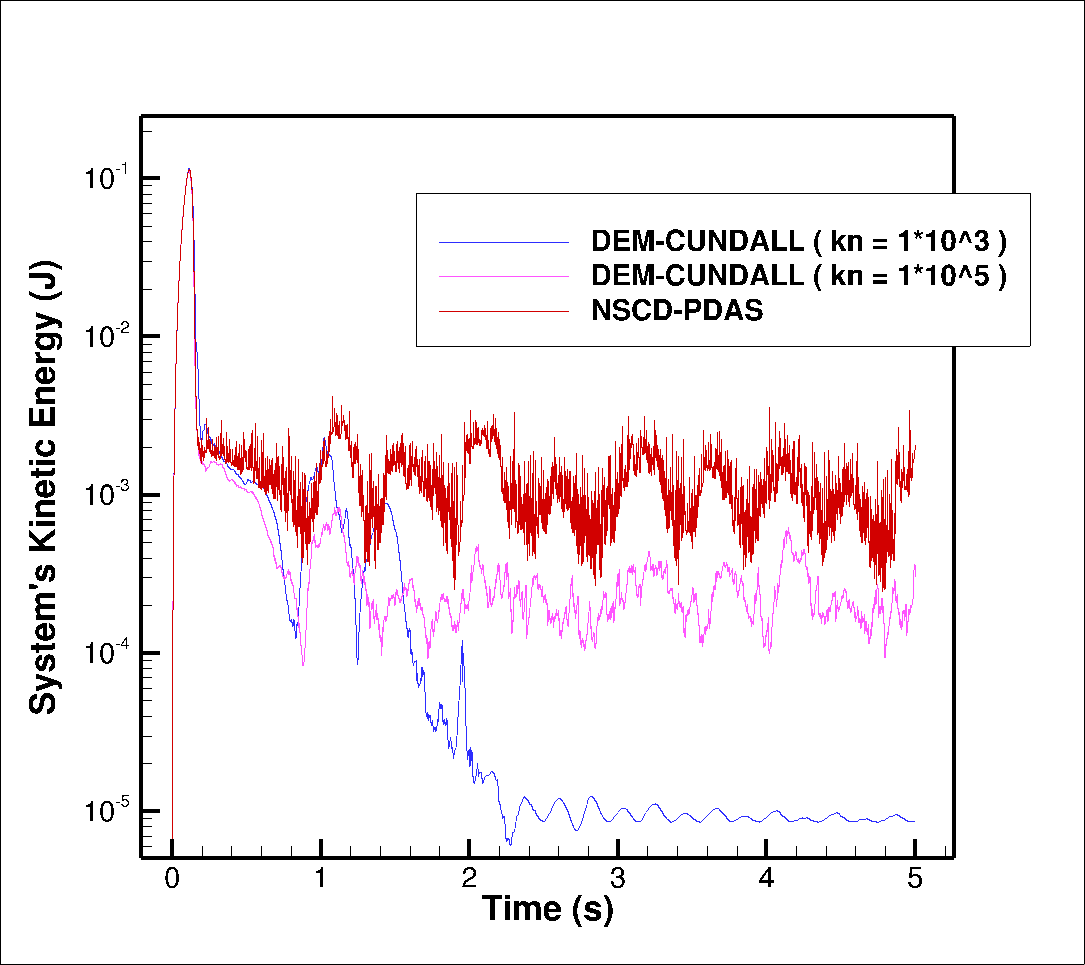
\includegraphics[width=0.55\textwidth]{chapitres/chapitre_4/figures/ec_tambour_400.png}
    \caption{\centering Variations de l'énergie cinétique des simulations d'écoulements granulaires dans un tambour rotatif à 400 particules de distribution aléatoire au cours du temps obtenues par DEM-CUNDALL (pour différentes constantes de raideur normales $k_n$) et NSCD-PDAS.}\label{fig134}
\end{figure}

La simulation d'un écoulement granulaire sur un petit système avec l'approche NSCD-PDAS permet donc de retrouver un profil d'écoulement similaire à celui obtenu par DEM-CUNDALL. La condition de persistance formulée dans le cadre de la NSCD assure à la fois une non-interpénétrabilité et une conservation de la quantité d'énergie en régime établi, en comparaison avec l'approche DEM-CUNDALL. Cette dernière approche, plus simple à mettre en oeuvre, est associée à des coûts de calculs important lorsque la constante de raideur normale est élevée, contrairement à l'approche NSCD-PDAS dont la mise en oeuvre algorithmique est certes plus complexe, mais dont la stabilité est plus étendue. 

\subsection{Performances et scalabilité}

L'objectif de cette partie est d'évaluer la scalabilité de la méthode NSCD-PDAS dans le cadre de son implémentation dans l'environnement MFiX-EXA. Pour rappel, MFiX-EXA offre la possibilité d'hériter du parallélisme et permet de traiter des écoulements granulaires sur des systèmes à grande échelle. Dans cette perspective, nous considérons une extension du cas-test précédent avec plus de particules et de contacts simultanés. Une collection de plus de $16000$ particules de diamètres uniformément distribués entre $1$ et $2$ $mm$ est déposée au fond d'un tambour de $450$ $mm$ de diamètre de vitesse de rotation égale à $40 $ $rpm$. Pour ce cas-test, une première simulation a été réalisée pour atteindre un écoulement en régime établi, caractérisé par un grand nombre de contacts simultanés. Ensuite, les simulations ont été réalisé à partir de ce régime en augmentant le nombre de sous-domaines afin de réduire la taille du problème local sur chaque sous-domaine et relever les temps CPU pour chaque approche. Les résultats, obtenus avec le supercalculateur HPC@LR, ont été réalisé sur $4$, $8$, $16$, $32$, $64$ et $96$ CPU. La répartition des particules et des contacts en sous-domaines de calcul associés aux différents processeurs physiques est faite suivant la grille de partitionnement présentée dans la Table \ref{tab_49}. Les paramètres physiques et numériques de la simulation sont reportés dans les Tables ci-dessous: 

\begin{center}
\begin{table}[!h]
\begin{tabular}{ |p{6.5cm}|p{6.1cm}| }
 \hline \rowcolor{lightgray}
 Paramètre& Valeur\\
 \hline
 Rayons particules  ($mm$) & $r = [1 - 2]$\\
 Densité volumique ($Kg.m^{-3}$)& $\rho = 2700$\\
 Diamètre du tambour ($mm$) & $D_{drum} = 450$\\
 Vitesse de rotation du tambour ($rpm$) & $\Omega_{drum} = 40$\\
 Vitesse initiale  ($m.s^{-1}$)  &$v_0 = 0$\\
 Force de gravité ($m.s^{-2}$)& $g = -9.80665$\\
 Masse de la particule ($Kg$)  &$m_p = \rho \pi r_p^{2}$\\
 \hline
\end{tabular}
\caption{Paramètres physique de la simulation d'écoulement granulaire dans un tambour rotatif.}\label{tab_47}
\end{table}
\end{center}

\vspace{-1cm}

\begin{center}
\begin{table}[!h]
\begin{tabular}{ |p{5cm}|p{3.8cm}|p{3.4cm}| }
 \hline \rowcolor{lightgray}
 DEM-CUNDALL& NSCD-PDAS& Communs\\
 \hline
 $e_n = 0.59$ & $e_n = 0.46$ & $T = 1 \quad s$\\
 $k_n = 10^4 \quad N.m^{-1}$& $e_t = 1$ & -\\
 $\eta_{ratio} = 0.5$ & $\gamma_n = 10^{-8}$ & $\mu = 0.2$\\
 $k_t = \frac{2}{7} k_n$ & $\gamma_t = 10^{-8}$ & -\\
 - & $\epsilon_{NLGS} =  10^{-8}$ & -\\
 $dt \approx 3.8\times10^{-6} \quad s$ &$dt = 1\times10^{-5} \quad s$ &-\\
 \hline
\end{tabular}
\caption{Paramètres numériques pour la simulation d'écoulement granulaire dans un tambour rotatif pour chaque approche de contact.}\label{tab_48}
\end{table}
\end{center}

\vspace{-1.5cm}

\begin{center}
\begin{table}[!h]
\begin{tabular}{ |p{6.5cm}|p{6.1cm}| }
 \hline \rowcolor{lightgray}
 Nombre de processeurs& Grille de partitionnment $(n_x\times n_y)$\\
 \hline
 $1$ & $1\times1$\\
 $4$& $2\times2$\\
 $8$ & $4\times2$\\
 $16$ & $4\times4$\\
 $32$ & $8\times4$\\
 $64$ & $8\times8$\\
 $96$ & $12\times8$\\
 \hline
\end{tabular}
\caption{Décompositions du domaine de calcul suivant le nombre de processeurs attribués au système parallèle.}\label{tab_49}
\end{table}
\end{center}

\vspace{-1cm}

La Figure \ref{tambour_16000} montre les profils d'écoulements granulaires obtenues par la méthode NSCD-PDAS. Sur les Figures \ref{tambour_16000_dem_diam-2} et \ref{tambour_16000_dem_rank-2}, on observe une pente caractéristique du régime établi. De plus, les niveaux de couleur présentés dans les Figures \ref{tambour_16000_dem_rank-1} et \ref{tambour_16000_dem_rank-2} illustrent la décomposition géométrique type cartésienne proposée par MFiX. On notera par ailleurs que la distribution des particules n'est pas homogène, des processeurs n'étant pas affectés par des particules lors de la simulation. 

\begin{figure*}[h!]
   \subfloat[\label{tambour_16000_dem_diam-1}]{%
      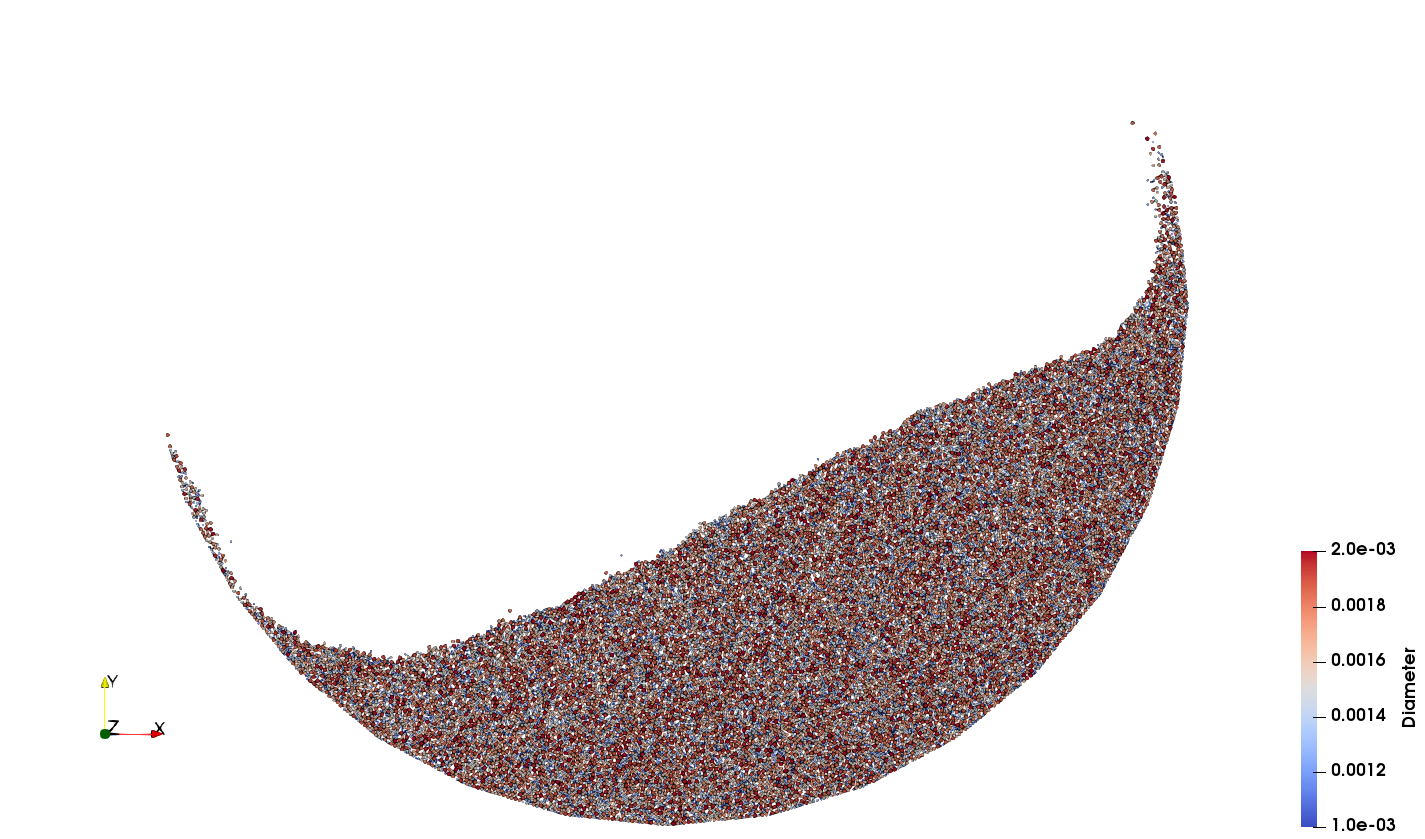
\includegraphics[trim=100 20 10 60,clip, width=0.5\textwidth]{chapitres/chapitre_4/figures/DEM_tambour-16000_diameter_1.png}}
\hspace{\fill}
   \subfloat[\label{tambour_16000_dem_diam-2}]{%
      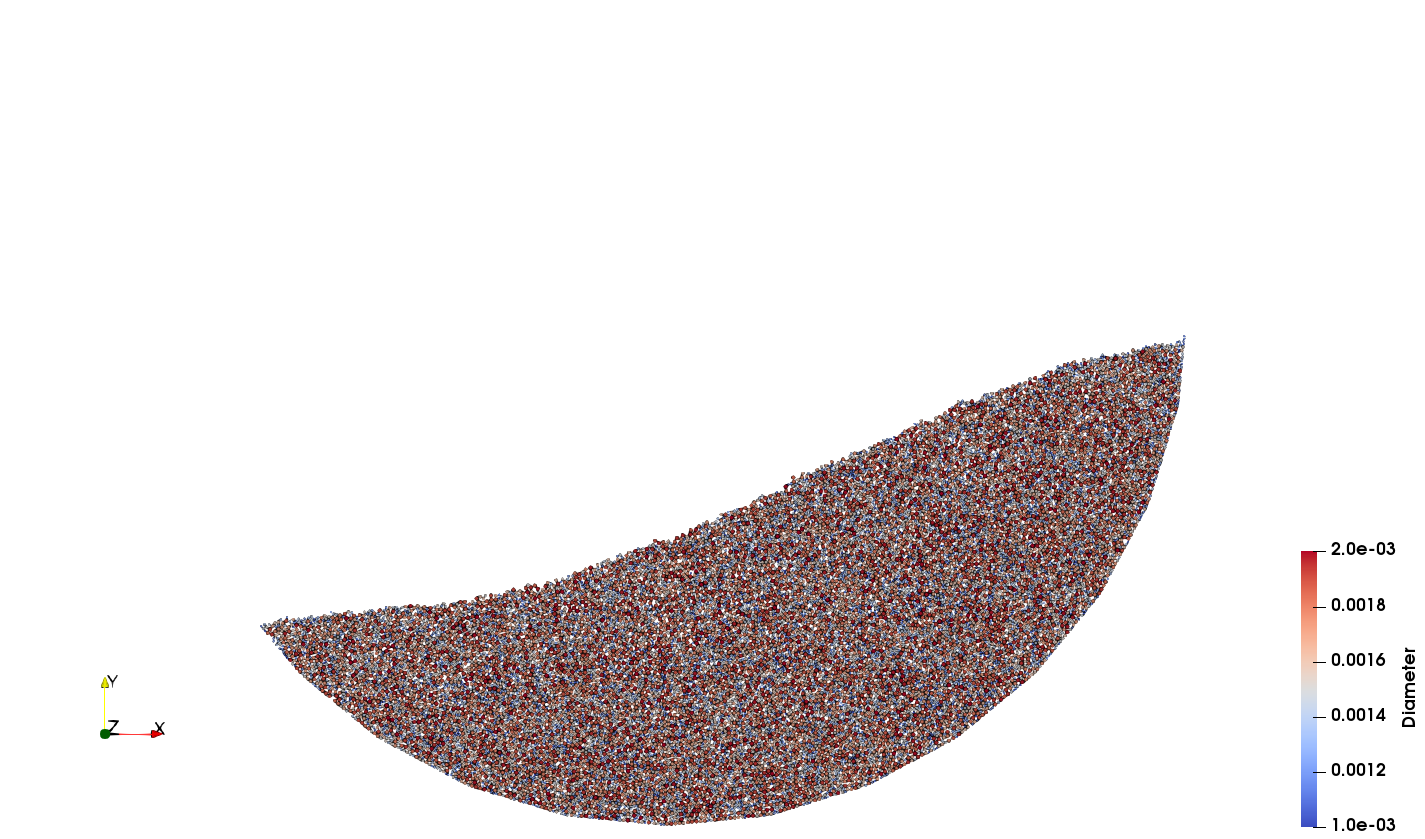
\includegraphics[trim=100 20 10 60,clip, width=0.5\textwidth]{chapitres/chapitre_4/figures/DEM_tambour-16000_diameter_2.png}}\\
\hspace{\fill}
   \subfloat[\label{tambour_16000_dem_rank-1}]{%
      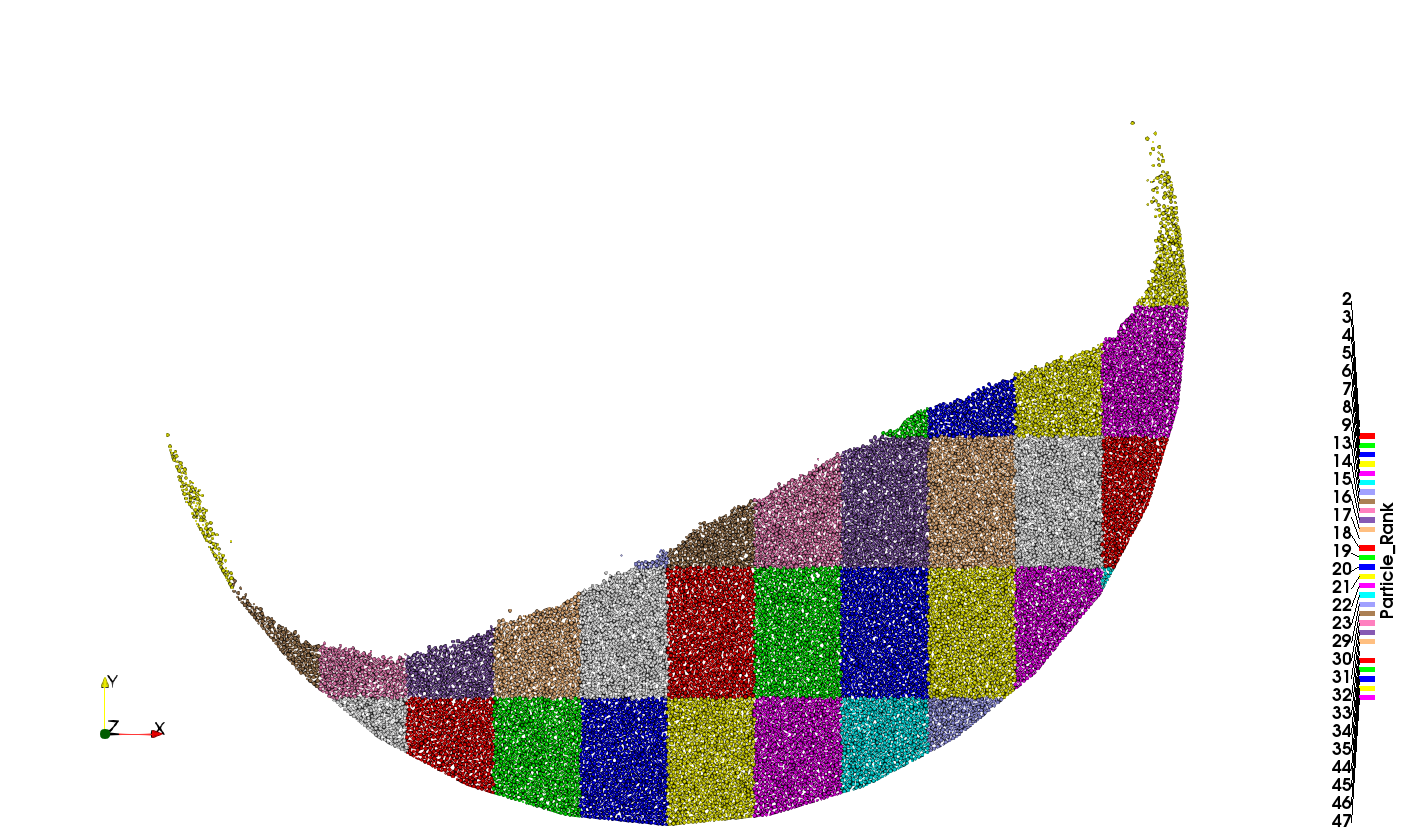
\includegraphics[trim=100 20 10 60,clip, width=0.5\textwidth]{chapitres/chapitre_4/figures/DEM_tambour-16000_rank_1.png}}
\hspace{\fill}
   \subfloat[\label{tambour_16000_dem_rank-2}]{%
      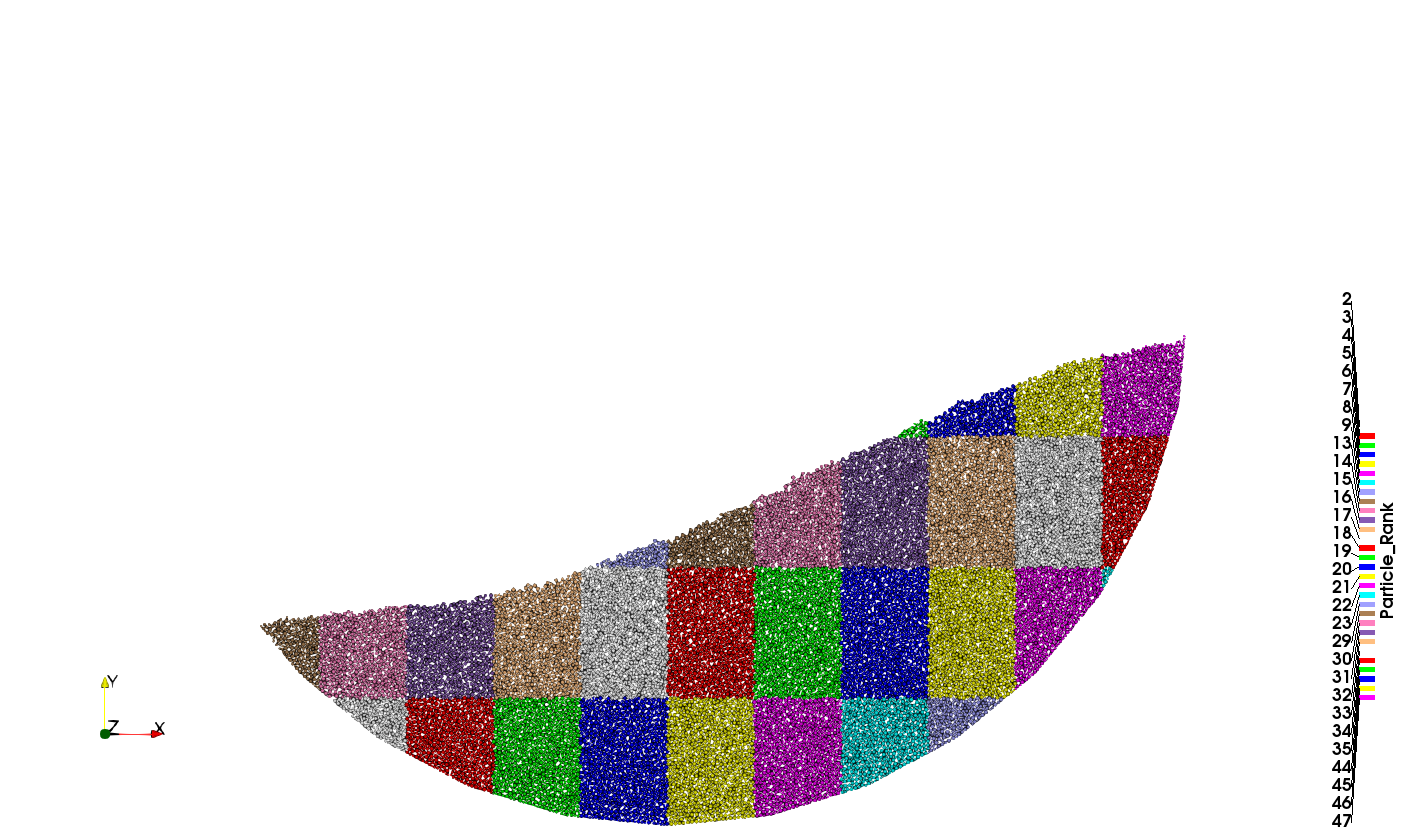
\includegraphics[trim=100 20 10 60,clip, width=0.5\textwidth]{chapitres/chapitre_4/figures/DEM_tambour-16000_rank_2.png}}\\
\caption{\label{tambour_16000}Instantanées des profils d'écoulements granulaires dans un tambour rotatif à plus de 16000 particules de distribution aléatoire uniforme obtenues par NSCD-PDAS [(a) et (b): diamètre des particules [(c) et (d): rang des processeurs] en régime transitoire [(a) et (c)] et régime établi [(b) et (d)].}
\end{figure*}

 Afin d'évaluer la scalabilité des deux approches, nous mesurons le "Speedup", défini comme le rapport du temps d'exécution en série de l'algorithme séquentiel pour résoudre un problème au temps mis par l'algorithme parallèle pour résoudre le même problème sur $p$ processeurs. En notant $T_s$ le temps d'exécution en série et $T_p$ le temps d'exécution parallèle, le Speedup est défini comme suit:
 
 \begin{equation}
     S = \frac{T_s}{T_p}
 \end{equation}
 
 L'autre indicateur de performance pertinent à déterminer pour ce cas-test est "l'Efficacité", définie comme le rapport du Speedup au nombre de processeurs. Cet indicateur mesure la fraction de temps pendant laquelle un processeur est utilisé:

 \begin{equation}
     E = \frac{S}{p} = \frac{T_s}{pT_p}
 \end{equation}

Pour les deux approches DEM-CUNDALL et NSCD-PDAS, les temps CPU relevés correspondent aux temps nécessaires pour réaliser 10 itérations temporelles. Les graphes de la Figure \ref{tambour_16000_speedup-efficiency} présentent la scalabilité obtenue pour l'écoulement.

\begin{figure*}[h!]
   \subfloat[\label{tambour_16000_speedup}]{%
      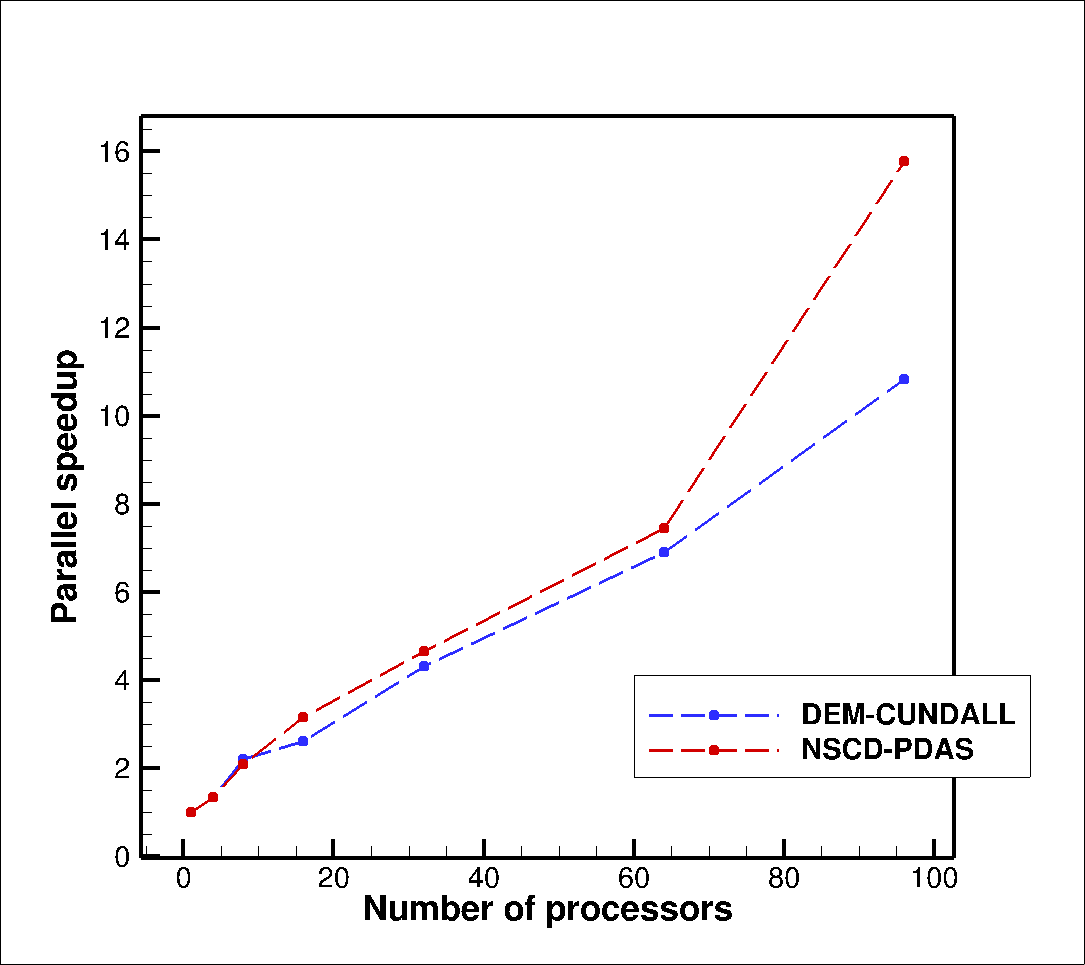
\includegraphics[trim=50 20 10 60,clip, width=0.5\textwidth]{chapitres/chapitre_4/figures/speedup_tambour_bis.png}}
\hspace{\fill}
   \subfloat[\label{tambour_16000_efficiency}]{%
      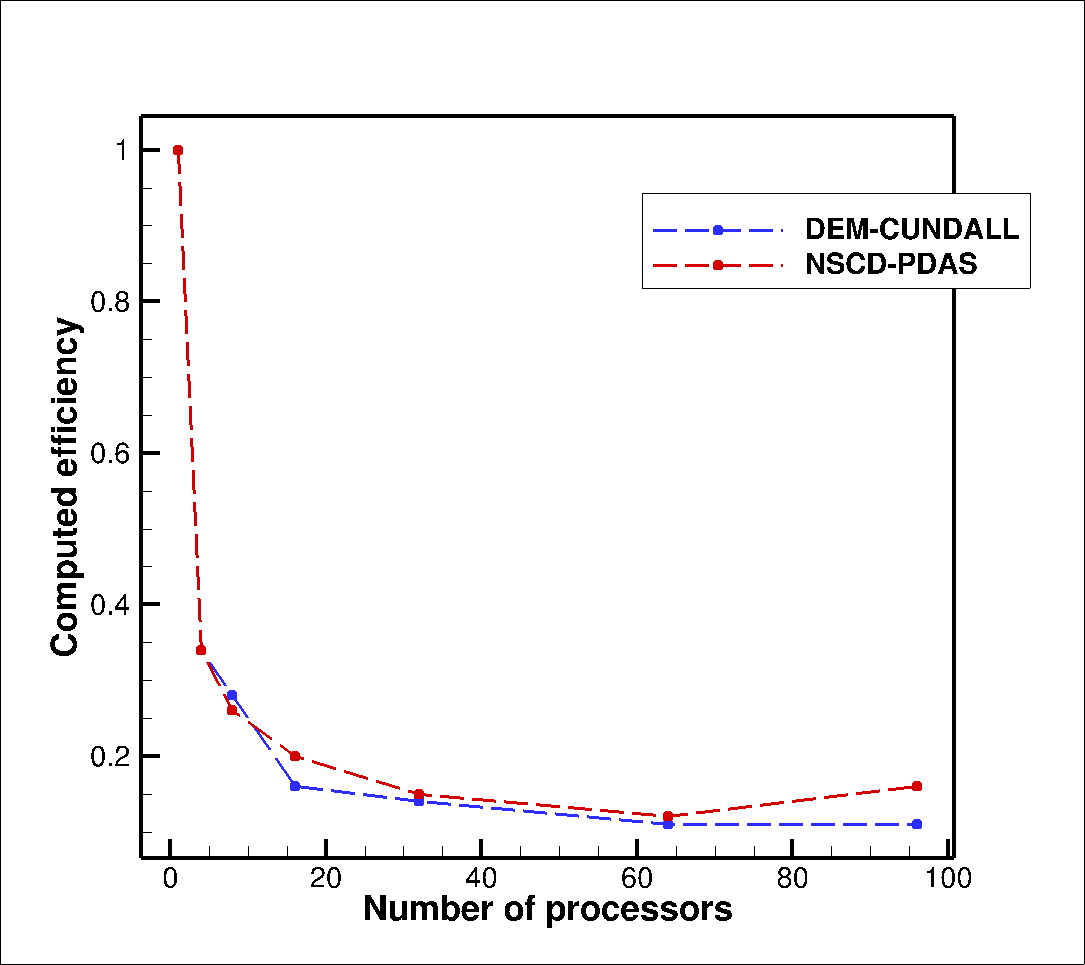
\includegraphics[trim=50 20 10 60,clip, width=0.5\textwidth]{chapitres/chapitre_4/figures/efficiency_tambour_bis.png}}\\
\caption{\label{tambour_16000_speedup-efficiency}Scalabilité obtenue par DEM-CUNDALL et NSCD-PDAS [(a) Speedup, (b) Efficacité en fonction du nombre de processeurs] mesurée à régime établi pour le système d'écoulement granulaire dans un tambour rotatif.}
\end{figure*}

Le graphe \ref{tambour_16000_speedup} représente l'évolution du speedup en fonction du nombre de processeurs, égale au nombre de sous-domaines. Les résultats montrent alors que la scalabilité du système parallèle avec l'approche NSCD-PDAS est identique à celle obtenue avec l'approche DEM-CUNDALL, l'augmentation du speedup par rapport au nombre de processeurs étant légèrement importante avec la NSCD. En terme d'efficacité (Figure \ref{tambour_16000_efficiency}), plus on augmente le nombre de processeurs, plus l'efficacité décroît.\\

De manière générale, les résultats obtenus pour l'approche NSCD-PDAS sont décevants. Cela s'explique notamment par le paradigme de parallélisation de MFiX qui repose sur un partitionnement cartésien géométrique du domaine de calcul, tel que présenté dans la Table \ref{tab_49}, et qui n'offre pas un équilibrage de la charge de calcul entre les différents processeurs, comme on peut le constater dans la Figure \ref{tambour_16000_dem_rank-2} en régime établi. Il s'ensuit inévitablement une perte d'efficacité. Le choix d'un tel paradigme de parallélisation dans MFiX est justifié dans le sens où les écoulements étudiés sont dispersés avec des charges de calcul équilibrées. On peut d'ailleurs dire que l'on exploite correctement le parallélisme proposé par MFiX puisque les résultats obtenus montrent que la méthode NSCD-PDAS utilise correctement l'outil existant avec des performances identiques en terme de scalabilité comparé à la DEM.

\section{Simulations numériques d'écoulements fluide-particules}\label{section_fluide}

Dans cette dernière partie, nous nous intéressons aux écoulements diphasiques fluide-particules. Cette perspective est possible car nous avons choisi MFiX-EXA comme environnement de développement de la méthode NSCD-PDAS. Nous allons présenter dans ce qui suit une étude de faisabilité de modélisation d'un écoulement fluide-particules. Cela va nous permettre de montrer comment la NSCD-PDAS permet de relaxer la contrainte de stabilité pour ce type de simulations.

\subsection{Éléments bibliographiques}

L'étude des écoulements fluide-particules consiste à prédire la dynamique d'un fluide dans lequel un ensemble de particules est en suspension.
La complexité de telles études réside en la combinaison  du caractère multi-échelles inhérent à l'écoulement fluide, de la dynamique de contact  particulaire et des échanges de quantité de mouvement entre les phases fluides et solides. Ces éléments de modélisation physique conduisent à différents modèles et donc différentes techniques de résolution numérique.
Ainsi, une classification naturelle se dégage en fonction de la dimension caractéristique des particules et de leur fraction de vide.\\

Le modèle deux fluides "Two-Fluid Model" (TFM) de type Euler-Euler, présenté par Gidaspow \cite{gidaspow1994multiphase, enwald1996eulerian}, est régulièrement utilisé pour simuler les écoulements diphasiques fluides-particules. Cette approche purement eulérienne des phases est construite sur une vision continue de la phase solide qui se mélange continûment avec la phase fluide. Cette hypothèse induit par construction une perte d'information des interactions particule-particule, qu'il convient de modéliser. On trouve des applications pour les lits fluidisés dans les références suivantes \cite{godlieb2009and, cloete2013generality, wang2015numerical}. Cette approximation de la phase solide permet de modéliser des systèmes à grandes échelles et offre des gains en temps de calcul, et c'est d'ailleurs les raisons pour lesquelles ce type de modèle est souvent utilisé dans des codes de calcul industriels, tels que MFiX-EXA.\\

La deuxième approche communément utilisée repose sur le principe du modèle Euler-Lagrange. Introduite par Tsuji, Kawaguchi et Tanaka \cite{tsuji1993discrete}, cette approche consiste en un couplage de la méthode des éléments discrets pour la modélisation des particules et de l'approche eulérienne de la phase fluide (CFD-DEM). Dans ce cas, la phase solide est considérée comme un ensemble de particules interagissant avec la phase fluide continue. Selon que l'écoulement soit plus ou moins chargé en particules, on dispose de différentes interactions selon le modèle de couplage \cite{elghobashi1991particle}; du fluide vers les particules (One-way coupling), fluide-particule réciproques (Two-way coupling) et fluide-particules réciproques ainsi que particules-particules (Four-way coupling). Dans la suite de cette partie, nous considérons les interactions de type Four-way coupling.\\

Dans le cadre de l'approche Euler-Lagrange qui traite les deux phases séparément, la quantité de mouvement échangée est calculée pour chaque
particule en fonction des informations provenant du fluide environnant. Partant de ce principe, deux techniques différentes peuvent être adoptées pour représenter la phase solide en formulation lagrangienne. La première consiste à considérer des particules immergées dans le fluide, de diamètre plus grand que la taille des cellules du maillage fluide. L'objectif étant de déterminer l'écoulement autour de la particule. La plateforme Xper \cite{perales2017xper, dbouk2016df} pour la simulation numérique d'interactions multi-physiques entre corps, repose sur ce même principe de granulat immergé. Les méthodes de frontière immergées (en anglais "Direct-Forcing Immersed Boundary Method" DF-IBM) y sont implémentées en combinant la description lagrangienne type NSCD pour les particules immergées et l'approche eulérienne basée sur les équations de Navier-Stokes pour la discrétisation fluide. La seconde technique, que l'on retrouve notamment dans MFiX-EXA \cite{garg2012documentation}, consiste quant à elle à représenter des particules de diamètre plus petit par rapport à la résolution du maillage fluide afin de déterminer l'influence des différentes interactions exercée par le fluide sur les particules. Cela permet notamment de modéliser des écoulements fluide-particules à grandes échelles.\\

Dans ce qui suit, on se restreint à cette approche qui est directement héritée du choix de MFiX-EXA et nous illustrons cela sur une simulation de lit fluidisé bidimensionnel dont le principe consiste à injecter sous un lit de matériaux granulaires, généralement de tailles comprises entre $15 \mu m$ et $6 mm$, un fluide sous pression. Ce fluide va alors soulever et disperser les particules constituant le lit par l'action d'une force de traînée opposée à la gravité. Ce genre de dispositif est utilisé dans de nombreuses  applications dans l'industrie, parmi lesquelles les procédés de dépollution par lit fluidisé, ou encore les réacteurs à lit fluidisé, où le combustible solide est fluidisé par l’introduction d’air dans un lit.

\subsection{Modèle mathématique et implémentation}

\subsection*{Équations de la dynamique de la phase fluide}

Le formalisme CFD-DEM a été proposée par Tsuji {\it et al.} \cite{tsuji1992lagrangian}, \cite{kawaguchi1998numerical}. Dans cette approche, le mouvement des particules discrètes est décrit par l'approche DEM-Cundall sur la base des lois de mouvement de Newton appliquées aux particules individuelles et à l'écoulement du fluide continu par la CFD basée sur les équations de Navier–Stokes. D'une part, les équations régissant la phase solide sont les mêmes que celles décrites en (\ref{eq_solide1})--(\ref{eq_solide3}). D'autre part, celles qui régissent la phase fluide pour la conservation de la masse et de la quantité de mouvement sont similaires à celles utilisées par les solveurs CFD classiques mais avec des termes de couplage supplémentaires dus aux forces de traînée agissant sur la phase solide. Anderson et Jackson \cite{anderson1967fluid} stipulent par ailleurs que dans le but de décrire de façon adaptée les écoulements granulaires, la dynamique de la phase fluide doit être calculée à partir des équations de Navier-Stokes moyennées en volume, en remplaçant ainsi les variables ponctuelles telles que
la vitesse, la pression, etc. par des champs localement filtrés et moyennés dans chaque cellule de la grille CFD. La fraction volumique de chaque cellule est alors définie par le nombre de particules présentes dans la cellule, comme cela a été décrit dans \cite{garg2012documentation}:

\begin{equation} \label{eq_fluide1}
\frac{\partial(\epsilon_f \rho_f)}{\partial t} + \vect{\nabla} . (\epsilon_f \rho_f \vect{v}_f) = 0 ;
\end{equation}

\begin{equation} \label{eq_fluide1}
\frac{\partial(\epsilon_f \rho_f \vect{v}_f)}{\partial t} = \vect{\nabla} . \overline{\overline{S}}_f + \epsilon_f \rho_f  \vect{g} - \Sigma_{m=1}^{M}\vect{I}_{fm} .
\end{equation}

Dans les équations ci-dessus, $\epsilon_f$ est la fraction volumique de la phase fluide, $\rho_f$ la densité thermodynamique de la phase fluide, $\vect{v}_f$ la vitesse moyenne en volume de la phase fluide, $\vect{I}_{fm}$ la quantité de mouvement entre le fluide et la phase solide $m$, et $\overline{\overline{S}}_f$ le tenseur de contrainte de la phase fluide défini par

\begin{equation} \label{eq_fluide1}
\overline{\overline{S}}_f = -P_f \overline{\overline{I}} + \overline{\overline{\tau}}_f,
\end{equation}

où $P_f$ représente la pression de la phase fluide, et $\overline{\overline{\tau}}_f$ le tenseur de cisaillement,

\begin{equation} \label{eq_fluide1}
\overline{\overline{\tau}}_f = 2 \mu_f \overline{\overline{D}}_f + \lambda_f \vect{\nabla} . tr(\overline{\overline{D}}_f) \overline{\overline{I}},
\end{equation}

où $\overline{\overline{D}}_f = \frac{1}{2}[\vect{\nabla} \vect{v}_f + (\vect{\nabla} \vect{v}_f)^{T}]$ est le tenseur relatif au taux de déformation, et $\mu_f$ (respectivement $\lambda_f$) est le coefficient de viscosité dynamique (respectivement le second coefficient de viscosité) de la phase fluide. Le couplage fluide-particules se fait par le biais de la quantité de mouvement échangée ($\Sigma_{m=1}^{M}\vect{I}_{fm}$) entre le fluide et la phase solide.\\ 

\subsection*{Estimation de la quantité de mouvement}

Pour des raisons de clarté, nous considérons dans ce paragraphe  une seule particule $p$ se trouvant à l'instant $t$ dans une cellule fluide $k$. Pour estimer la quantité de mouvement $\vect{I}_{fm}$ échangée entre le fluide et la particule $p$ appartenant à la phase solide $m$ dans le cadre d'un couplage CFD-DEM, il est nécessaire de calculer au niveau de cette cellule, la force de traînée vue en (\ref{eq_solide2}), c'est à dire la force du fluide agissant sur cette particule. L'expression de cette force est donnée par la formule suivante: 

\begin{equation} \label{drag_force}
\vect{F}_d^{(p \in k,m)} = \vect{\nabla} P_f(\vect{X}^{(p)})\nu_m + \frac{\beta_m^{(p \in k)}\nu_m}{\epsilon_{sm}}\Bigg[\vect{v}_f(\vect{X}^{(p)})-\vect{V}^{(p)}\Bigg]
\end{equation}

\noindent où $P_f(\vect{X}^{(p)})$ et $\vect{v}_f(\vect{X}^{(p)})$ représentent les champs de pression et de vitesse moyens au niveau de la particule, $\nu_m$ le volume de la particule $p$, et $\beta_m^{(p \in k)}$ le coefficient de transfert de la quantité de mouvement entre le fluide et la particule $p$.\\

Cette force de traînée, calculée pour une seule particule, permet de déterminer la quantité de mouvement $\vect{I}_{fm}^k$ échangée entre le fluide dans la cellule $k$ et la particule $p$ de la façon suivante:

\begin{equation} \label{fm_momentum}
\vect{I}_{fm}^k = \frac{1}{\nu_k}\vect{F}_d^{(p \in k,m)}K(\vect{X}_m^{(p)},x_k)
\end{equation}

\noindent où $x_k$ désigne les coordonnées du centre de la cellule fluide $k$, $\nu_k$ le volume de la cellule fluide $k$ et $K(\vect{X}_m^{(p)},x_k)$ un noyau générique à support compact qui détermine l'influence de la force exercée par la particule $p$ de coordonnées $\vect{X}_m^{(p)}$ sur la cellule fluide $k$. Lorsqu'il s'agit de considérer plusieurs particules par cellule fluide, les forces de traînée exercées sur chaque particules sont sommées pour déterminer la quantité de mouvement échangée par cellule.

\subsection*{Schéma de couplage CFD-DEM}

Au vu de la dynamique de la phase fluide et des échanges de quantité de mouvement effectués avec la phase solide, le couplage CFD-DEM se fait à deux niveaux. D'abord au niveau local sur chacune des particules constituant la phase solide, et ensuite au niveau des cellules de la grille CFD où l'écoulement de la phase fluide est calculé par les équations de Navier-Stokes. Dans le cadre d'un écoulement dans un lit fluidisé par exemple, des échanges sont régulièrement effectués entre les deux phases. Le couplage CFD-DEM étant explicite, les informations sont échangées au début du pas de temps. Le solveur CFD est avancé d'un pas de temps CFD $(dt_{CFD})$, puis les particules sont avancées au temps $(t+dt_{CFD})$. À cause du modèle qui impose des pas de temps petits, il est nécessaire de réaliser des sous pas de temps entre deux pas de temps fluide ($dt_{DEM}<dt_{CFD}$). La Figure \ref{schema_couplage} illustre de manière simplifiée le couplage fluide-particules dans MFiX-EXA. Le solveur CFD résout les équations de Navier-Stokes relatives à la phase fluide, et le solveur DEM traite le mouvement d'ensemble des particules constituant la phase solide.

\begin{figure}[!h]
  \centering
    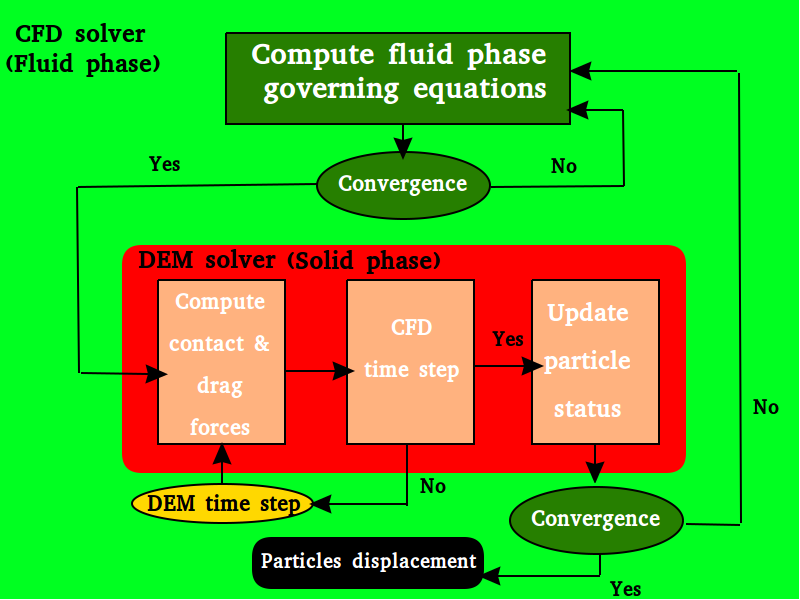
\includegraphics[width=0.6\textwidth]{chapitres/chapitre_4/figures/shema_couplage.png}
    \caption{\centering Schéma simplifié du couplage CFD-DEM.}\label{schema_couplage}
\end{figure}

Dans les modèles de contact à sphère-souple type CUNDALL, le pas de temps $dt_{DEM}$ requis pour le calcul des impulsions de contact entre les particules de la phase solide dépend de la constante de raideur normale choisie (voir équation \ref{t_coll}). Celle-ci, déterminée à partir des propriétés physiques des matériaux utilisés, influe considérablement sur la dynamique de l'écoulement granulaire. Du fait que les temps de collision sont petits, et pour des raisons de stabilité numérique de la DEM, il est nécessaire d'avoir des pas de temps inférieurs au temps de collision. On a alors des pas de temps solides qui ont plusieurs ordres de grandeur plus petits que le pas de temps fluide ($dt_{DEM}<dt_{CFD}$). De ce fait, plus la constante de raideur normal $k_n$ est grande, plus les pas de temps sont petits, ce qui entraîne des temps de calculs longs. Cependant, dans le cas où l'on  considère un modèle de contact non-régulier NSCD, cette contrainte liée au temps de collision n'existe plus, le pas de temps solide peut être pris plus grand ($dt_{NSCD}>dt_{DEM}$), voire même égale au pas de temps fluide ($dt_{NSCD}=dt_{CFD}$).

\subsection{Application à la simulation d'un lit fluidisé}

L'objectif de cette partie est d'étudier l'écoulement d'un lit fluidisé, où un ensemble de grains est mis en mouvement par une circulation de fluide au niveau de la paroi inférieure, et ce, afin d'étendre l'utilisation de l'approche NSCD-PDAS à de nouvelles applications faisant intervenir un couplage fluide-particules. Dans cette perspective, nous allons nous intéresser à la simulation du lit fluidisé bidimensionnel dit de "Goldschmidt", et on se place dans le cadre de l'étude menée dans \cite{goldschmidt2004hydrodynamic} pour tester et évaluer les profils d'écoulements obtenus par DEM-CUNDALL et NSCD-PDAS.

\subsubsection{Description du cas-test}

On considère un lit fluidisé (cf. Figure \ref{maillage_lit}) constitué d'un canal vertical soumis à un flux d'air ascendant émis depuis sa partie inférieure. Initialement, la simulation du lit fluidisé de Goldschmidt "Pseudo-2D" réalisée dans \cite{goldschmidt2004hydrodynamic} contient environ vingt-cinq mille billes de verre réparties sur 4 rangées et initialisées avec une petite vitesse aléatoire. Dans notre cas bidimensionnel, nous considérons une seule rangée de billes, la profondeur du domaine de calcul étant prise égale au diamètre des billes sphériques. Le fluide et les billes solides sont confinés pour se déplacer uniquement dans le plan du calcul, ce qui réduit dans notre cas le nombre à un peu plus de $4000$ billes simulées. Par ailleurs, la vitesse d'entrée du jet central de fluide est augmentée linéairement sur une période d'une seconde. Un schéma simplifié de l'écoulement, ainsi que le maillage du conteneur, qui détermine la taille des mailles de la grille de calcul pour cet écoulement de particules mono-dispersés couplé au fluide, est illustré dans la Figure \ref{maillage_lit}.  Le paramètre d'espacement du maillage est donné par la formule suivante:

\vspace{-0.3cm}

\begin{equation}
    \Delta^* = \sqrt[3]{dx dy}/d_p
\end{equation}

\noindent où $d_p$ est le diamètre des particules. Une grille de $N_x \times N_y = 15 \times 45$ est alors appliquée, ce qui donne un espacement de grille sans dimension de $\Delta^* \approx 2$. Nous fournissons dans les Tables \ref{tab_fluide_phys} et \ref{tab_fluide_num} l'ensemble des paramètres physiques et numériques de ces simulations.

\begin{center}
\begin{table}[!h]
\begin{tabular}{ |p{7cm}|p{6cm}| }
 \hline \rowcolor{lightgray}

 Paramètre& Valeur\\
 \hline
 Dimensions du lit (L X H) ($mm \times mm$)& $150 \times 700$\\
 Taille du maillage fluide  & $15 \times 45$\\
 Dimension des cellules ($mm \times mm$)& $10 \times 15.6$\\
 Taille de la grille & $2.0$ \\
 Hauteur du lit statique ($mm \times mm$) & $220$\\
 Vitesse de fluidisation minimale ($m.s^{-1}$)&   $42$\\
 Nombre de particules& $N = 4107$\\
 Diamètre des particules ($mm$)& $d_p = 2.49$\\
 Densité des particules ($Kg.m^{-3}$)& $\rho_s = 2526$\\
 Densité du fluide ($Kg.m^{-3}$)& $\rho_f = 1.2\times10^{-3}$\\
 Viscosité du fluide ($N.m^{-2}$)& $\mu_f = 1.8\times10^{-5}$\\
 Force de gravité ($m.s^{-2}$)& $g = -9.80665$\\
 \hline
\end{tabular}
\caption{Paramètres physiques pour la simulation du lit fluidisé de Goldschmidt \cite{goldschmidt2004hydrodynamic}.}\label{tab_fluide_phys}
\end{table}
\end{center}

\vspace{-1cm}

\begin{figure}[!h]
  \centering
    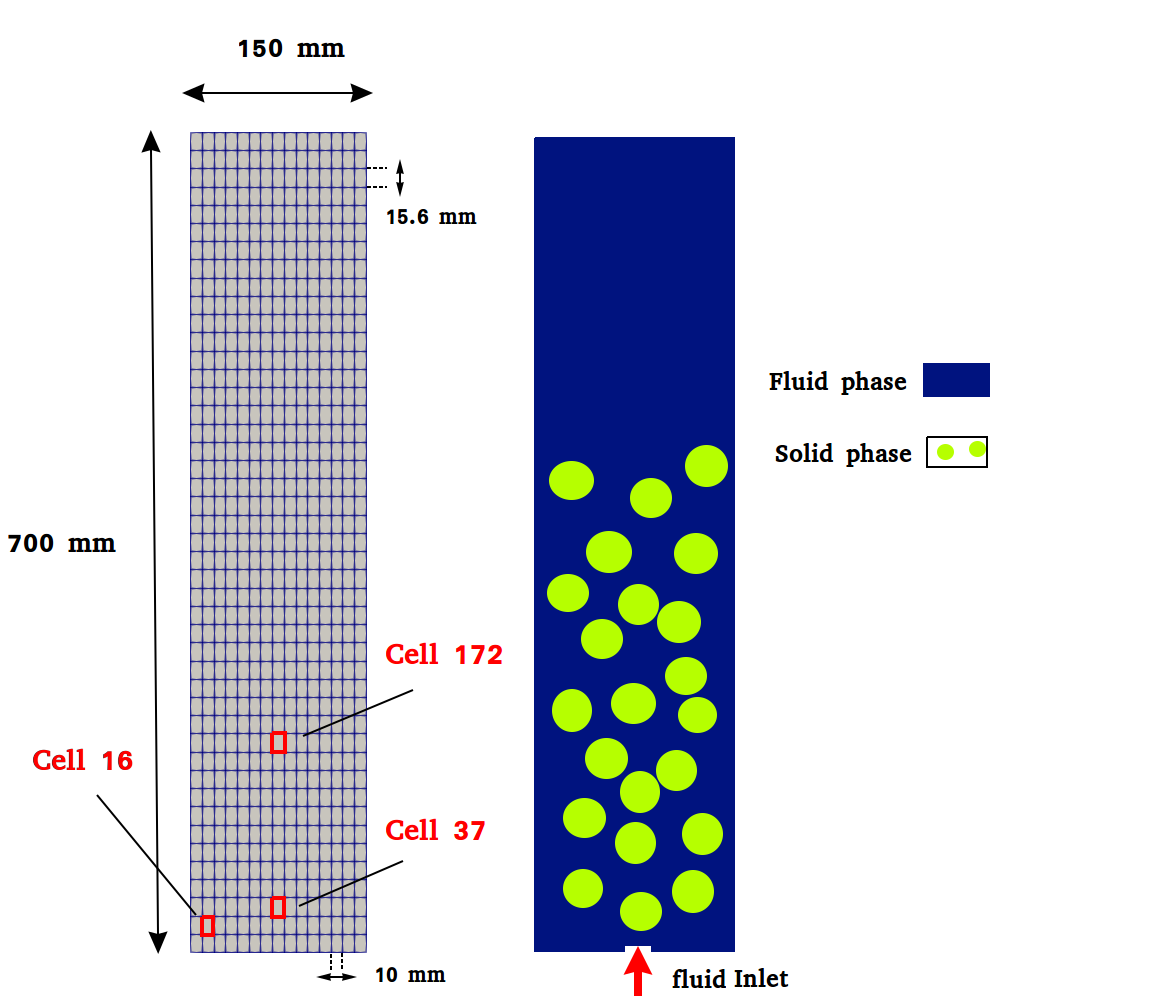
\includegraphics[width=0.65\textwidth]{chapitres/chapitre_4/figures/maillage.png}
    \caption{\centering Maillage fluide du conteneur (à gauche) et schématisation d'un écoulement fluide-particules de la simulation du lit fluidisé de Goldschmidt \cite{goldschmidt2004hydrodynamic}.}\label{maillage_lit}
\end{figure}

\vspace{-0.8cm}

\begin{center}
\begin{table}[!h]
\begin{tabular}{ |p{4.4cm}|p{4.2cm}|p{3.8cm}| }
 \hline \rowcolor{lightgray}
 DEM-CUNDALL& NSCD-PDAS& Communs\\
 \hline
 $e_n = 0.97$ & $e_n = 0.97$ & $T = 60 \quad s$\\
 $k_n = 2519 \quad N.m^{-1}$& $e_t = 1$ & -\\
 $k_t = \frac{2}{7} k_n \quad N.m^{-1}$ & $\gamma_n = 10^{-2}$ & $\mu = 0.1$\\
 $\eta_{ratio} = 0.5$ & $\gamma_t = 10^{-2}$ & -\\
 - & $\epsilon_{NLGS} =  10^{-4}$ & -\\
 - &- &$dt_{fl} = [5-10]\times10^{-4} s$\\
 $dt_{solide} \approx 4\times10^{-6} \quad s$ &$dt_{solide} = 1\times10^{-4} \quad s$ &-\\
 \hline
\end{tabular}
\caption{Paramètres numériques pour la simulation du lit fluidisé de Goldschmidt \cite{goldschmidt2004hydrodynamic} pour chaque approche de contact.}\label{tab_fluide_num}
\end{table}
\end{center}

\subsubsection{Dynamique de l'écoulement}

L'objectif de ce paragraphe est de donner un aperçu global de l'écoulement dans le lit fluidisé, indépendamment de l'approche utilisée. Pour cela, nous réalisons une simulation sur un temps d'intégration de $60$ secondes, assez long pour pouvoir observer un régime établi où le lit est en perpétuel mouvement. Nous constatons alors que l'écoulement se met en mouvement et tend vers un régime stationnaire au bout de quelques secondes de simulation. Par ailleurs, en se basant sur une comparaison qualitative des champs dit "instantanés" de vitesses des particules correspondants à la phase de fluidisation du lit (voir Figure \ref{granular_flow}), on observe les mêmes écoulements à différents instants de la simulation, aussi bien pour la DEM que pour la NSCD. Ces séquences temporelles montrent par ailleurs une faible présence du fluide près des parois inférieures du conteneur, la concentration de particules y est beaucoup plus élevée. Un phénomène de re-circulation se met en place, puisque les particules tassées au fond du lit passent par le centre du lit par où le fluide est injecté, puis sont éjectées vers les bords.

\begin{figure*}[h!]
   \subfloat[\label{granular_flow_dem_0s}]{%
      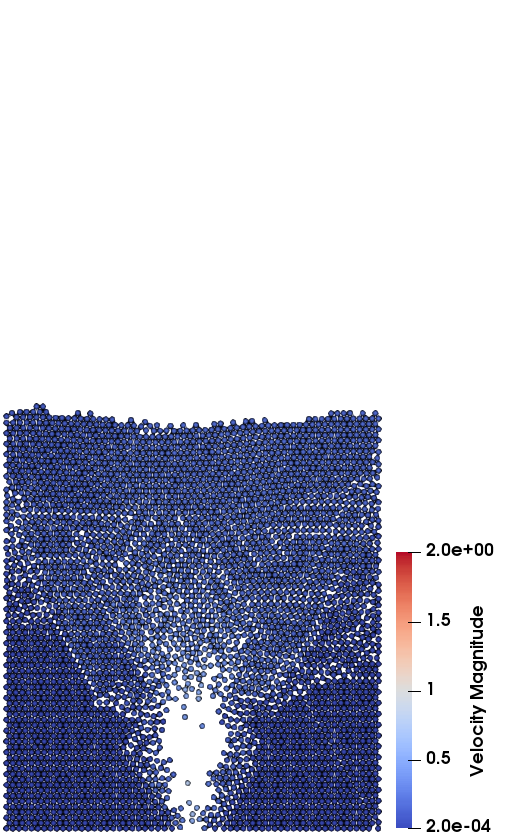
\includegraphics[width=0.185\textwidth]{chapitres/chapitre_4/figures/granular_flow_dem_0s.png}}
\hspace{\fill}
   \subfloat[\label{granular_flow_dem_1s}]{%
      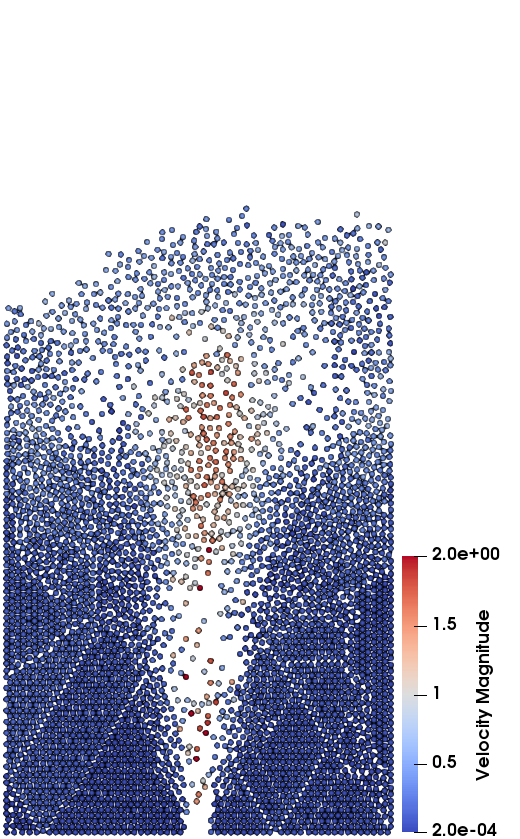
\includegraphics[width=0.185\textwidth]{chapitres/chapitre_4/figures/granular_flow_dem_1s.png}}
\hspace{\fill}
   \subfloat[\label{granular_flow_dem_60s}]{%
      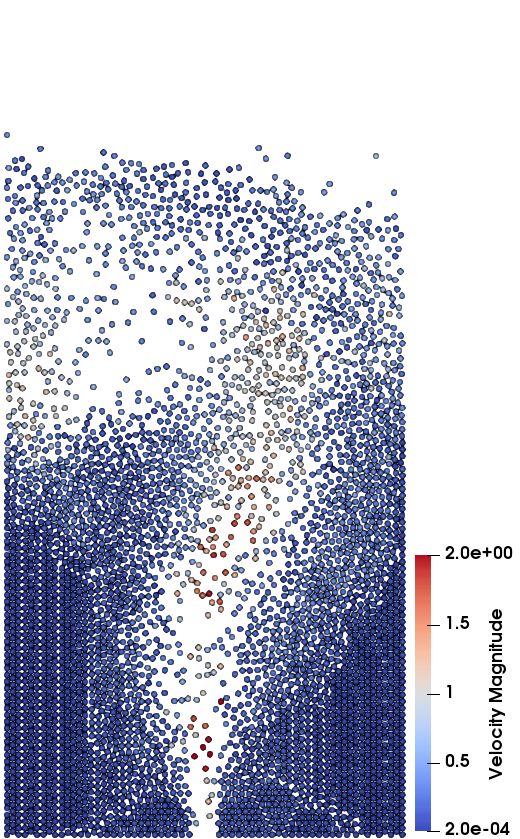
\includegraphics[width=0.185\textwidth]{chapitres/chapitre_4/figures/granular_flow_dem_60s.png}}\\
\subfloat[\label{granular_flow_dem_0s}]{%
      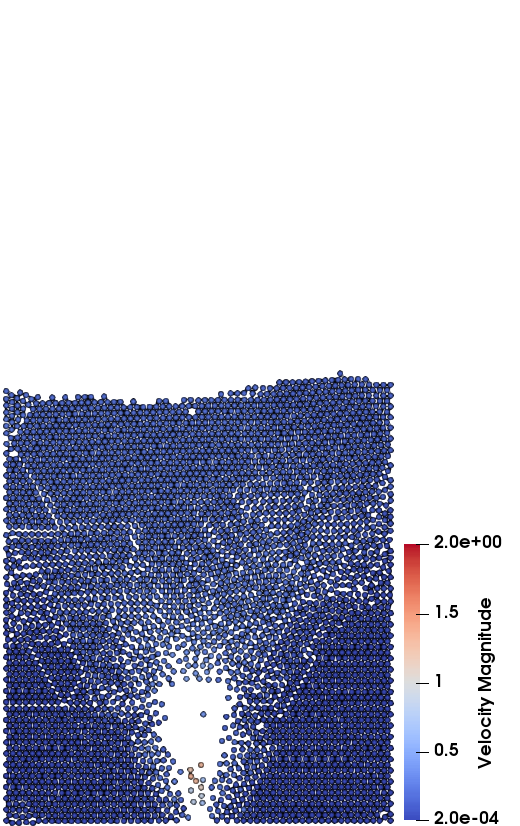
\includegraphics[width=0.185\textwidth]{chapitres/chapitre_4/figures/granular_flow_nscd_0s.png}}
\hspace{\fill}
   \subfloat[\label{granular_flow_nscd_1s}]{%
      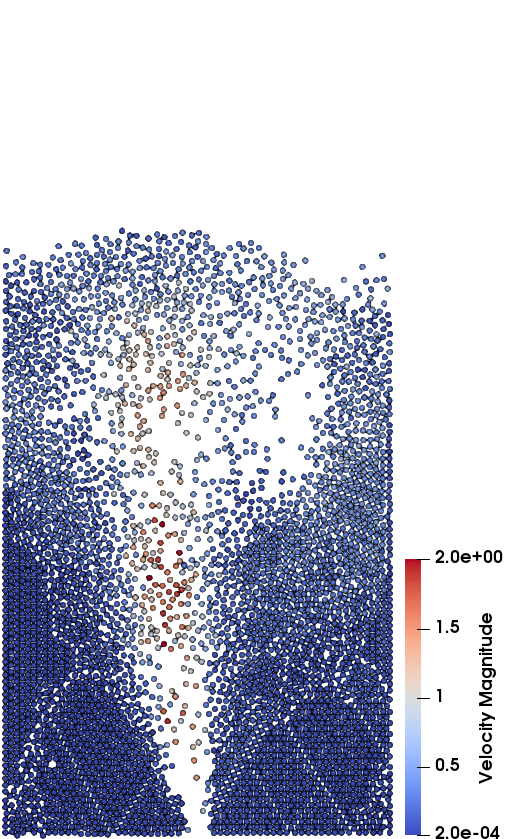
\includegraphics[width=0.185\textwidth]{chapitres/chapitre_4/figures/granular_flow_nscd_1s.png}}
\hspace{\fill}
   \subfloat[\label{granular_flow_nscd_60s}]{%
      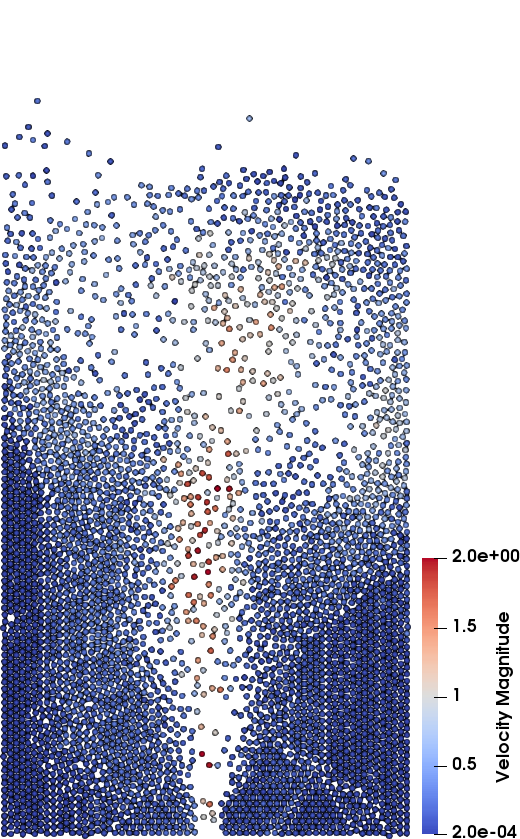
\includegraphics[width=0.185\textwidth]{chapitres/chapitre_4/figures/granular_flow_nscd_60s.png}}\\
\caption{\centering Champs instantanés de vitesses des particules soumises à jet central de fluide après 0.5 s (à gauche), 1 s (au milieu) et 60 s (à droite) de simulation obtenues par [(a), (b), (c)] DEM-CUNDALL, [(d), (e), (f)] NSCD-PDAS pour le lit fluidisé de Goldschmidt.}\label{granular_flow}
\end{figure*}

Nous fournissons également dans les graphes des Figures \ref{ep_g_data-time} et \ref{v_g_data-time} un échantillonnage de l'écoulement du fluide au cours du temps en $3$ points du maillage fluide (voir Figure \ref{maillage_lit}) en traçant pour chaque approche l'évolution temporelle des variables quantitatives relatives au fluide. Le caractère instationnaire de l'écoulement est alors observé, décrit par un signal fortement oscillatoire de la vitesse du fluide au cours du temps. Nous constatons de plus que la fraction volumique et la vitesse d'écoulement du fluide varient de manière très similaire pour les deux approches.

\begin{figure*}[h!]
   \subfloat[\label{ep_g_data-time_DEM}]{%
      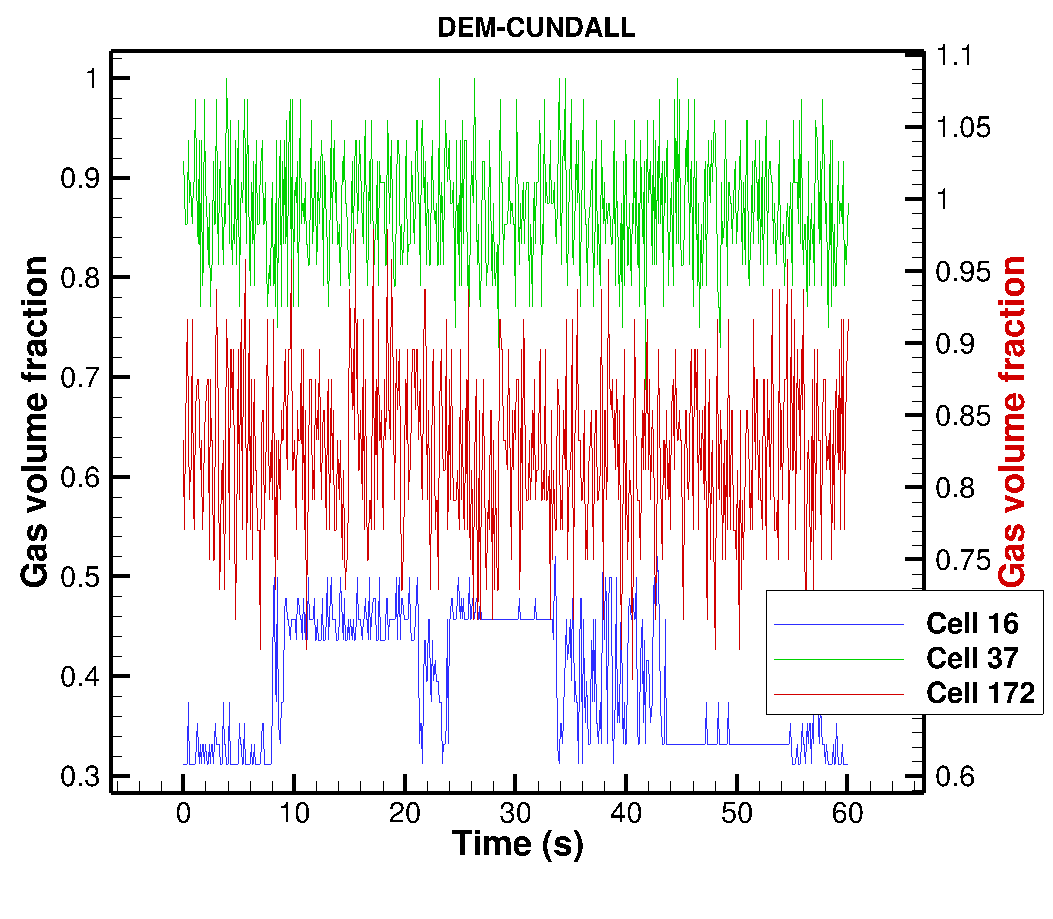
\includegraphics[width=0.5\textwidth]{chapitres/chapitre_4/figures/ep_g_data-time_DEM-CUNDALL.png}}
\hspace{\fill}
   \subfloat[\label{ep_g_data-time_PDAS} ]{%
      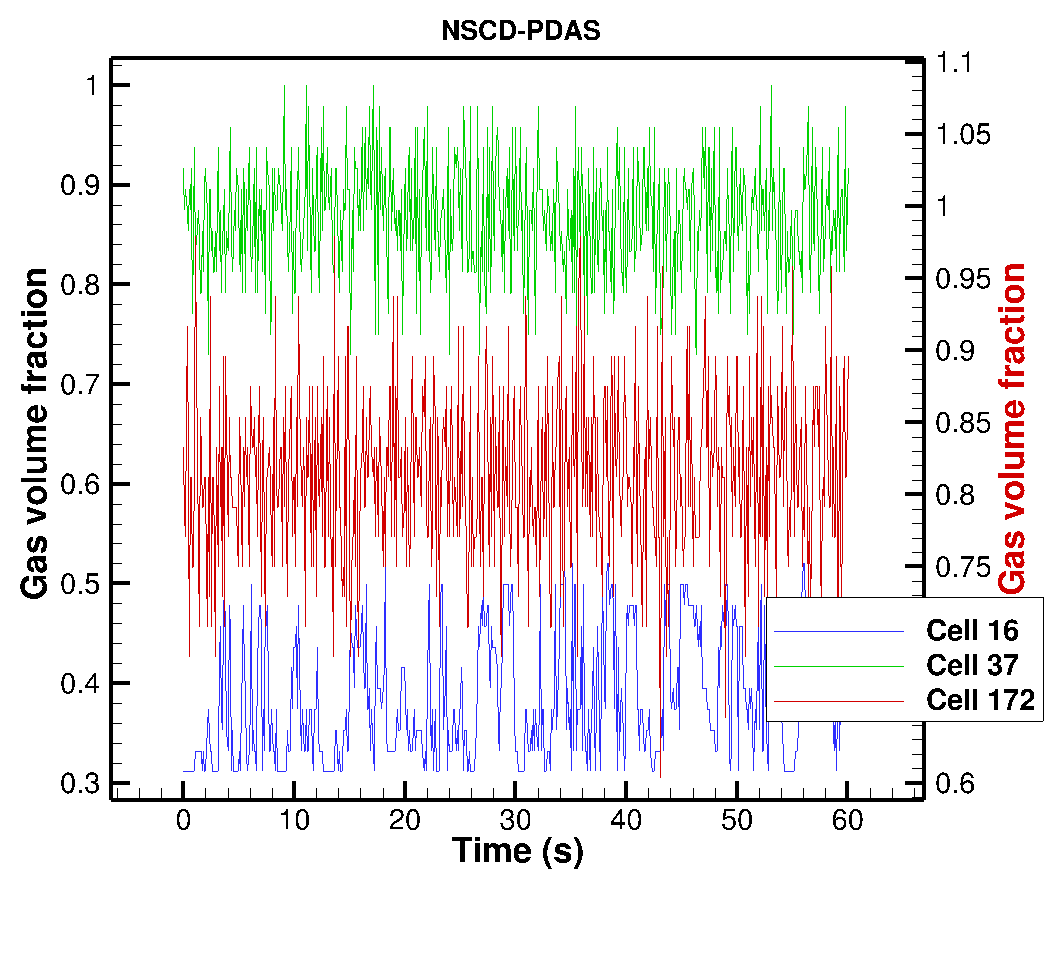
\includegraphics[width=0.5\textwidth]{chapitres/chapitre_4/figures/ep_g_data-time_NSCD-PDAS.png}}\\
\caption{\label{ep_g_data-time}Évolution de la fraction volumique du fluide au cours du temps dans différentes cellules du maillage fluide obtenues par (a) DEM-CUNDALL, (b) NSCD-PDAS pour le lit de Goldschmidt.}
\end{figure*}

\begin{figure*}[h!]
   \subfloat[\label{v_g_data-time_DEM}]{%
      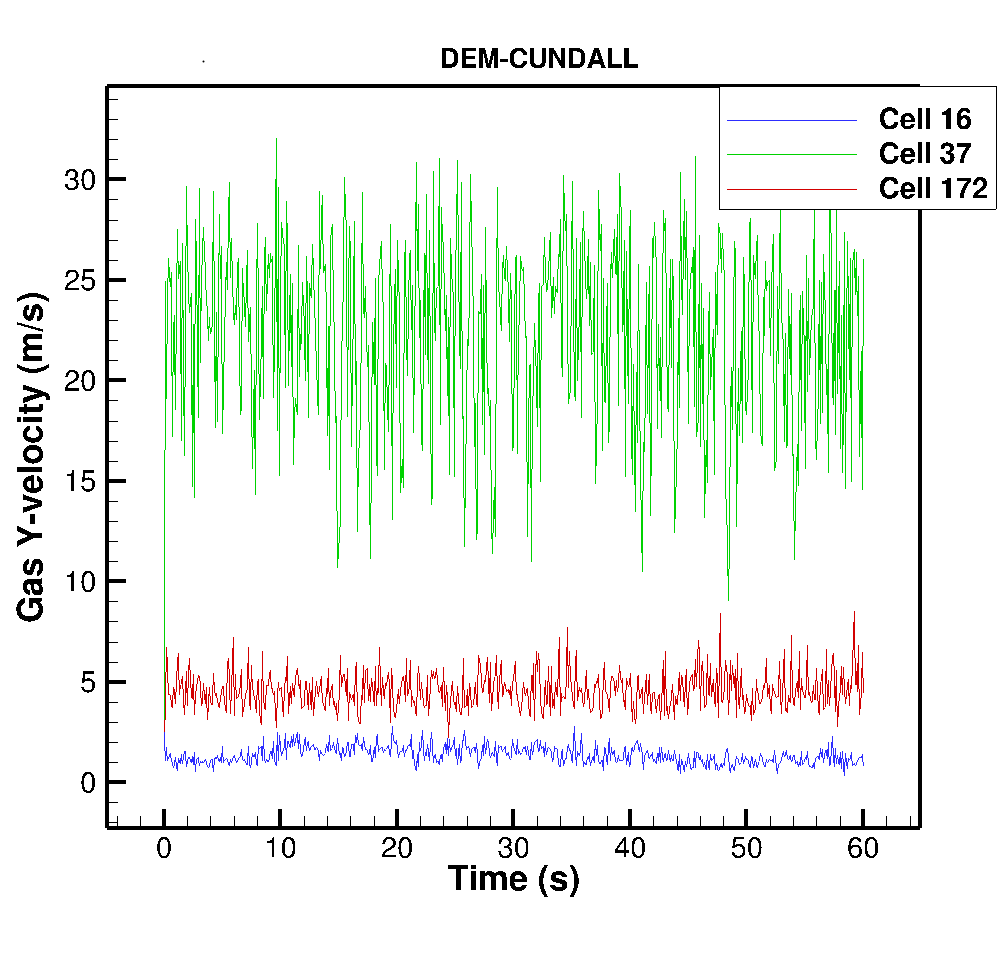
\includegraphics[width=0.5\textwidth]{chapitres/chapitre_4/figures/v_g_data-time_DEM-CUNDALL.png}}
\hspace{\fill}
   \subfloat[\label{v_g_data-time_PDAS} ]{%
      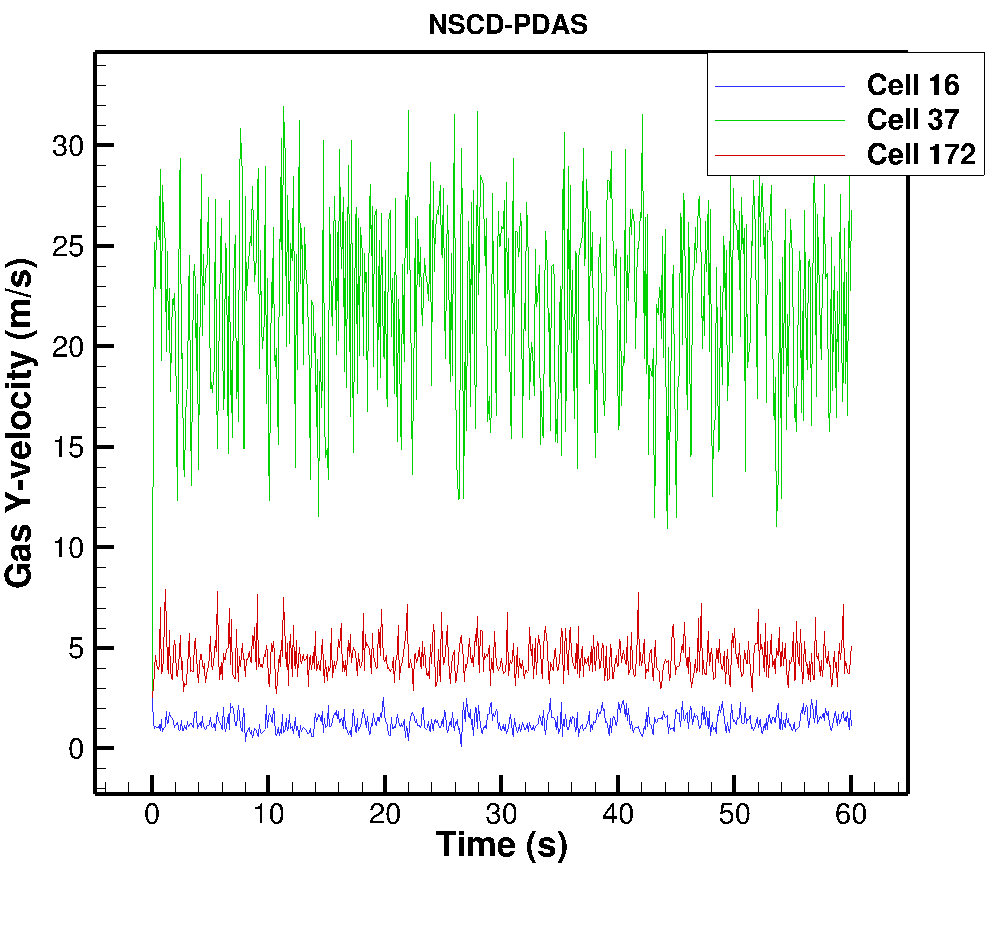
\includegraphics[width=0.5\textwidth]{chapitres/chapitre_4/figures/v_g_data-time_NSCD-PDAS.png}}\\
\caption{\label{v_g_data-time}Évolution de la vitesse d'écoulement du fluide au cours du temps dans différentes cellules du maillage fluide obtenues par (a) DEM-CUNDALL, (b) NSCD-PDAS pour le lit fluidisé de Goldschmidt.}
\end{figure*}

\subsubsection{Comparaisons quantitatives DEM-CUNDALL / NSCD-PDAS}
%\subsubsection{Comparaison des modèles d'écoulement fluide-particules}

On s'intéresse à présent aux grandeurs moyennes relatives aux modèles d'écoulements que nous allons comparer pour les deux approches DEM-CUNDALL et NSCD-PDAS. Pour cela, nous réalisons deux simulations et nous calculons à partir des champs instantanés de vitesses des particules présentés dans la Figure \ref{granular_flow} la fraction volumique moyenne du fluide pour un instant $t$ spatiale (en l'occurrence dans la Figure \ref{ep_g_60s} à $t = 60s$). En superposant ces deux champs avec ceux des Figures \ref{granular_flow_dem_60s} et \ref{granular_flow_nscd_60s} à $60$ secondes de simulation, nous observons des profils d'écoulements similaires.  

\begin{figure*}[h!]
\centering
   \subfloat[\label{ep_g_60s_dem}]{%
      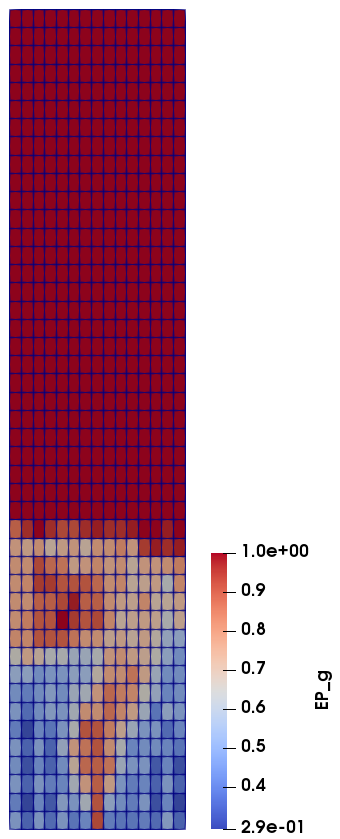
\includegraphics[width=0.25\textwidth]{chapitres/chapitre_4/figures/ep_g_60s_dem.png}}
\hspace{4em}%
   \subfloat[\label{ep_g_60s_nscd}]{%
      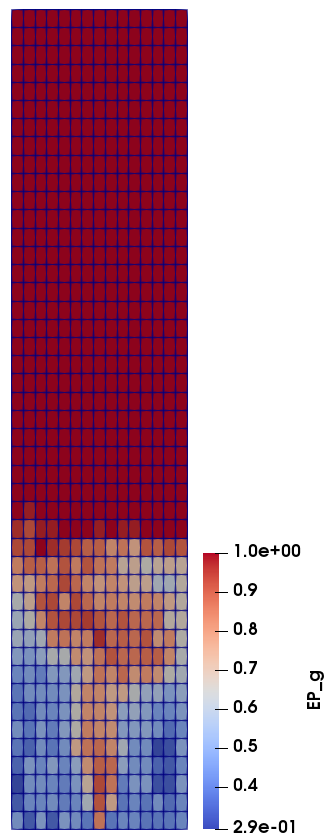
\includegraphics[width=0.25\textwidth]{chapitres/chapitre_4/figures/ep_g_60s_nscd.png}}\\
\caption{\centering Champs instantanés moyens en espace de la fraction volumique (a) DEM-CUNDALL, (b) NSCD-PDAS pour le lit fluidisé de Goldschmidt à 60 s de simulation.}\label{ep_g_60s}
\end{figure*}

En moyennant sur l'ensemble des échantillons obtenus sur un temps d'intégration de $60s$, nous obtenons les champs moyens dans le temps de la fraction volumique du fluide, décris dans les Figure \ref{ep_g_avg_dem} et \ref{ep_g_avg_nscd} pour l'approche DEM-CUNDALL et NSCD-PDAS respectivement. En procédant de façon similaire, nous obtenons les champs de vitesse moyennés dans le temps, comme représenté dans les Figures \ref{gas_vel_avg_dem} et \ref{gas_vel_avg_nscd} pour les deux approches.

\begin{figure*}[h!]
\centering
   \subfloat[\label{ep_g_avg_dem}]{%
      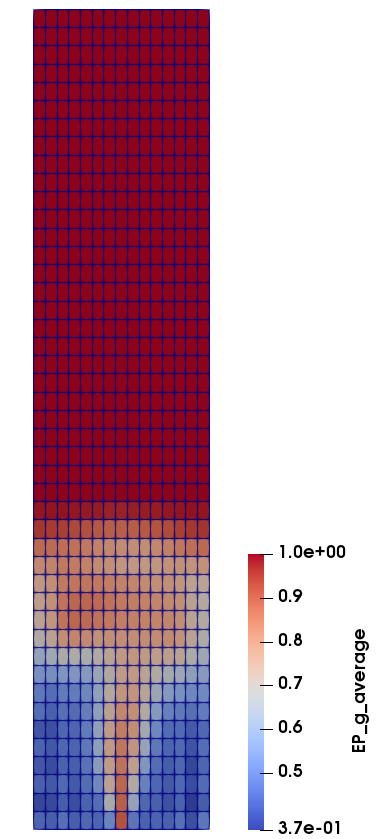
\includegraphics[width=0.25\textwidth]{chapitres/chapitre_4/figures/ep_g_avg_dem.png}}
\hspace{4em}%
   \subfloat[\label{ep_g_avg_nscd}]{%
      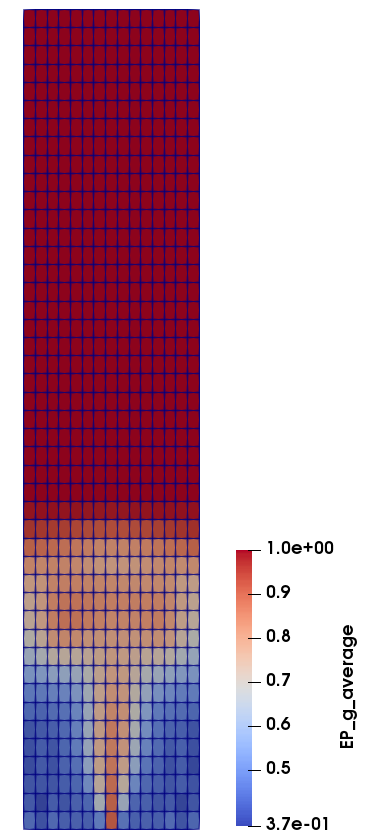
\includegraphics[width=0.25\textwidth]{chapitres/chapitre_4/figures/ep_g_avg_nscd.png}}\\

\centering
   \subfloat[\label{gas_vel_avg_dem}]{%
      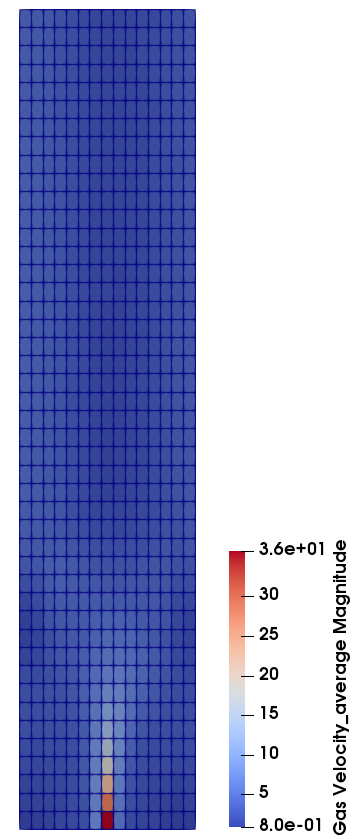
\includegraphics[width=0.25\textwidth]{chapitres/chapitre_4/figures/gas_vel_avg_dem.png}}
\hspace{4em}%
   \subfloat[\label{gas_vel_avg_nscd}]{%
      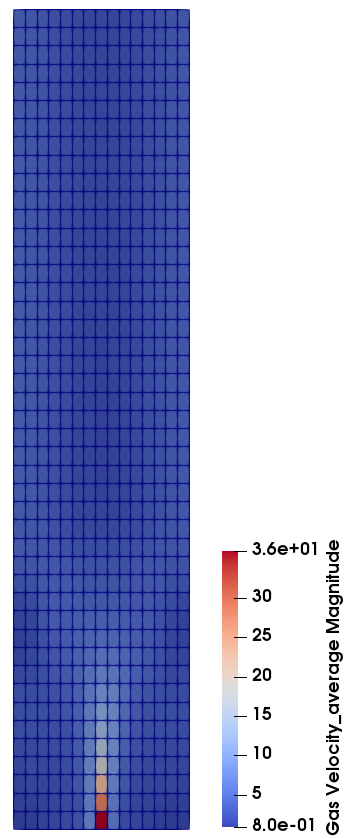
\includegraphics[width=0.25\textwidth]{chapitres/chapitre_4/figures/gas_vel_avg_nscd.png}}\\
\caption{\centering Champs moyens dans le temps de la fraction volumique et de la vitesse d'écoulement du fluide (a), (c) DEM-CUNDALL, (b), (d) NSCD-PDAS pour le lit fluidisé de Goldschmidt.}\label{lit_fluidisé}
\end{figure*}
\vspace{0.8cm}
Comme on peut le constater, ces résultats moyennés dans le temps sont qualitativement assez similaires pour les deux approches puisqu'on obtient les mêmes tendances de résultat. Pour pousser la comparaison encore plus loin, nous extrayons à partir des champs moyens précédemment présentés les profils d'écoulements des variables quantitatives moyennées dans le temps relatives au fluide. Nous procédons de façon à relever les profils à différentes hauteurs du lit, pour que la comparaison soit pertinente. Ainsi, les graphes des Figures \ref{ep_g_avg_data-profile_01}, \ref{ep_g_avg_data-profile_02} et \ref{ep_g_avg_data-profile_03} donnent les profils de fractions volumiques du fluide moyennées dans le temps pour le lit de Goldschmidt à différentes hauteurs. Les variations de ces profils sont assez similaires. À une hauteur $y = 0.1m$, les profils montrent une concentration élevée du fluide au milieu du lit avec un pic qui atteint une valeur de $ep_g = 0.8$, tandis que plus on se rapproche des parois, plus la concentration des particules est importante. Au delà de $y = 0.3m$, la concentration de particules est nulle pour les deux approches.

% -----------------------------------------------------
% -----------------------------------------------------
\begin{figure*}[h!]
   \subfloat[\label{ep_g_avg_data-profile_01}]{%
      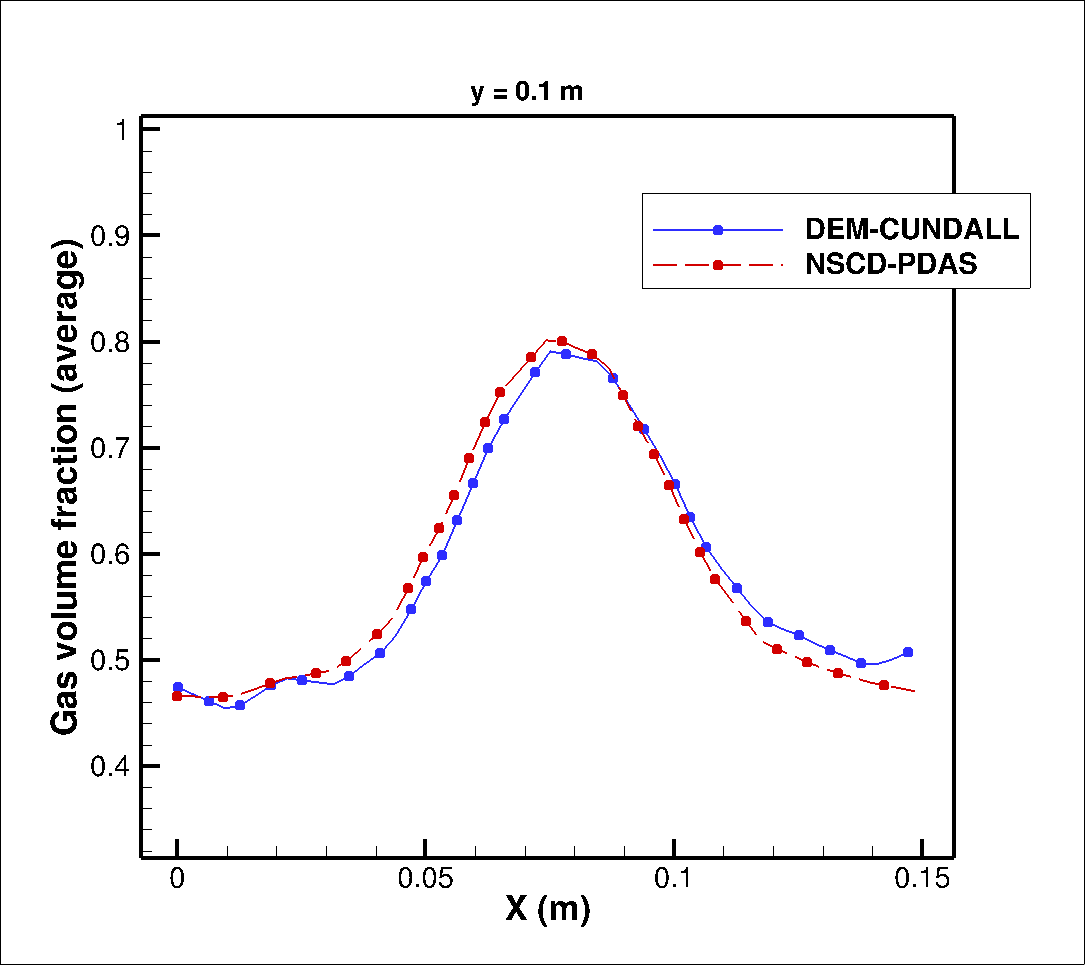
\includegraphics[trim=10 30 50 30,clip, width=0.32\textwidth]{chapitres/chapitre_4/figures/ep_g_avg_data-profile_01.png}}
\hspace{\fill}
   \subfloat[\label{ep_g_avg_data-profile_02} ]{%
      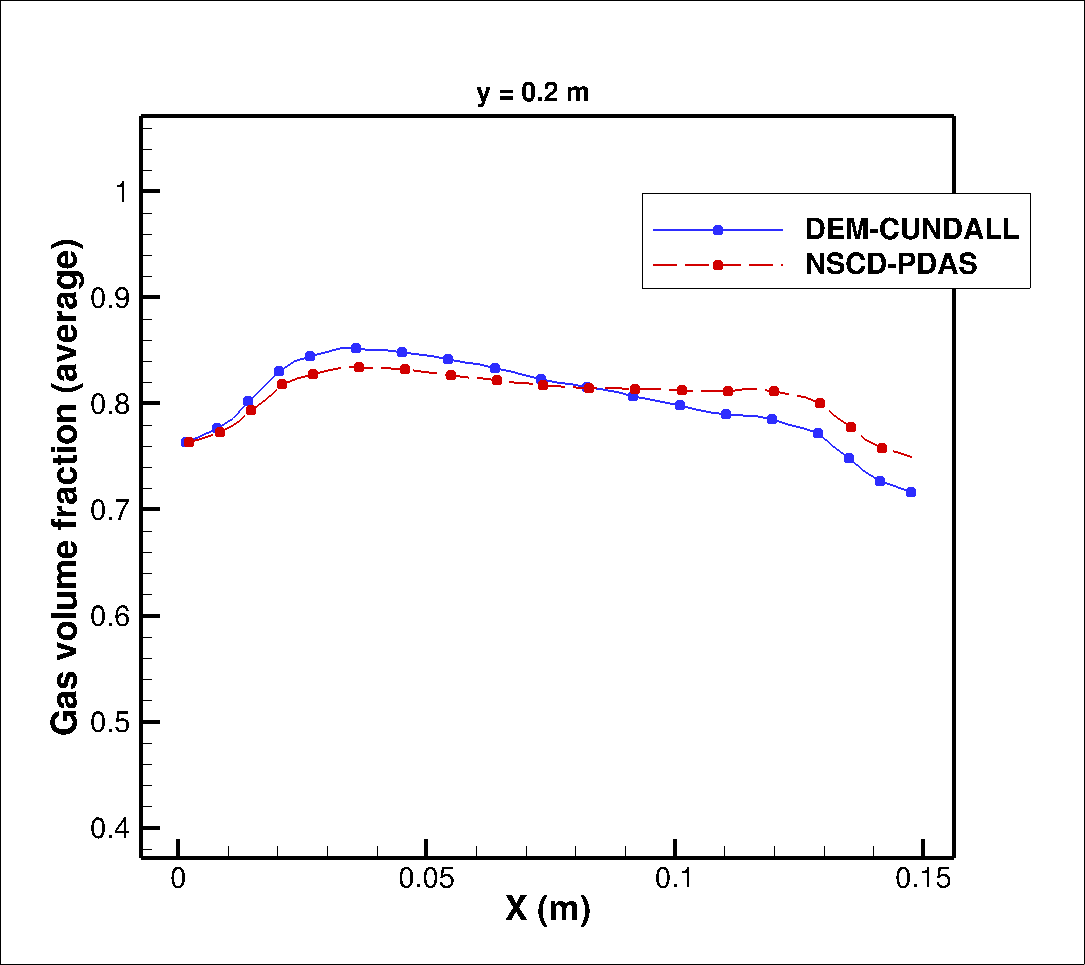
\includegraphics[trim=10 30 50 30,clip, width=0.32\textwidth]{chapitres/chapitre_4/figures/ep_g_avg_data-profile_02.png}}
\hspace{\fill}
   \subfloat[\label{ep_g_avg_data-profile_03} ]{%
      \centering 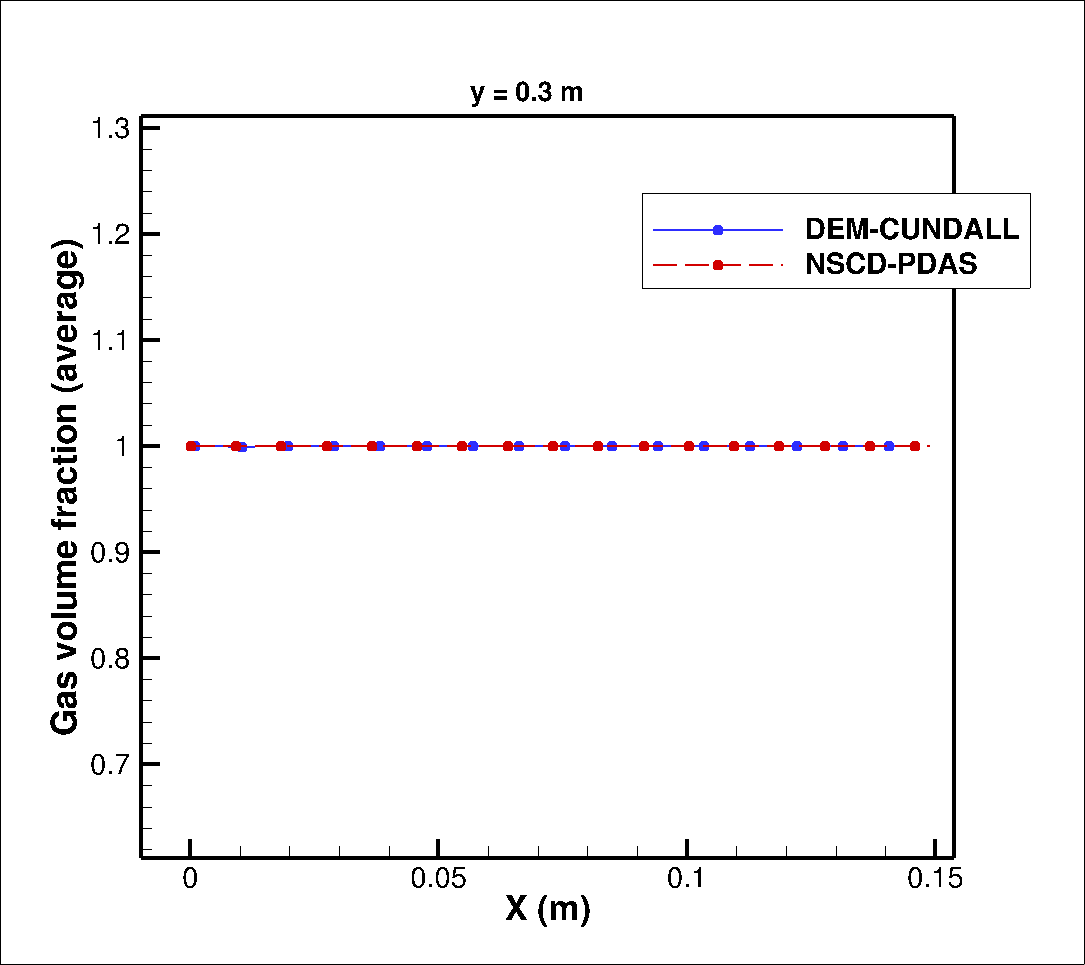
\includegraphics[trim=10 30 50 30,clip, width=0.32\textwidth]{chapitres/chapitre_4/figures/ep_g_avg_data-profile_03.png}}\\
\caption{\label{ep_g_avg_data-profile}Profils de fraction volumique du fluide moyennés dans le temps obtenus pour le lit fluidisé de Goldschmidt à différentes hauteurs. (a) $0.1 m$, (b) $0.2 m$, (c) $0.3 m$.}
\end{figure*}
% -----------------------------------------------------

Les profils de vitesses présentés dans les graphes des Figures \ref{v_g_avg_data-profile_01}, \ref{v_g_avg_data-profile_02} et \ref{v_g_avg_data-profile_03} sont également similaires pour les deux approches. Les particules sont éjectées au niveau de l'entrée du jet central de fluide, puis arrivées à une certaine hauteur limite, là où la vitesse du fluide devient assez faible pour ne plus entraîner les particules, retombent le long des parois du lit (voir Figure \ref{granular_flow}).

\begin{figure*}[h!]
   \subfloat[\label{v_g_avg_data-profile_01}]{%
      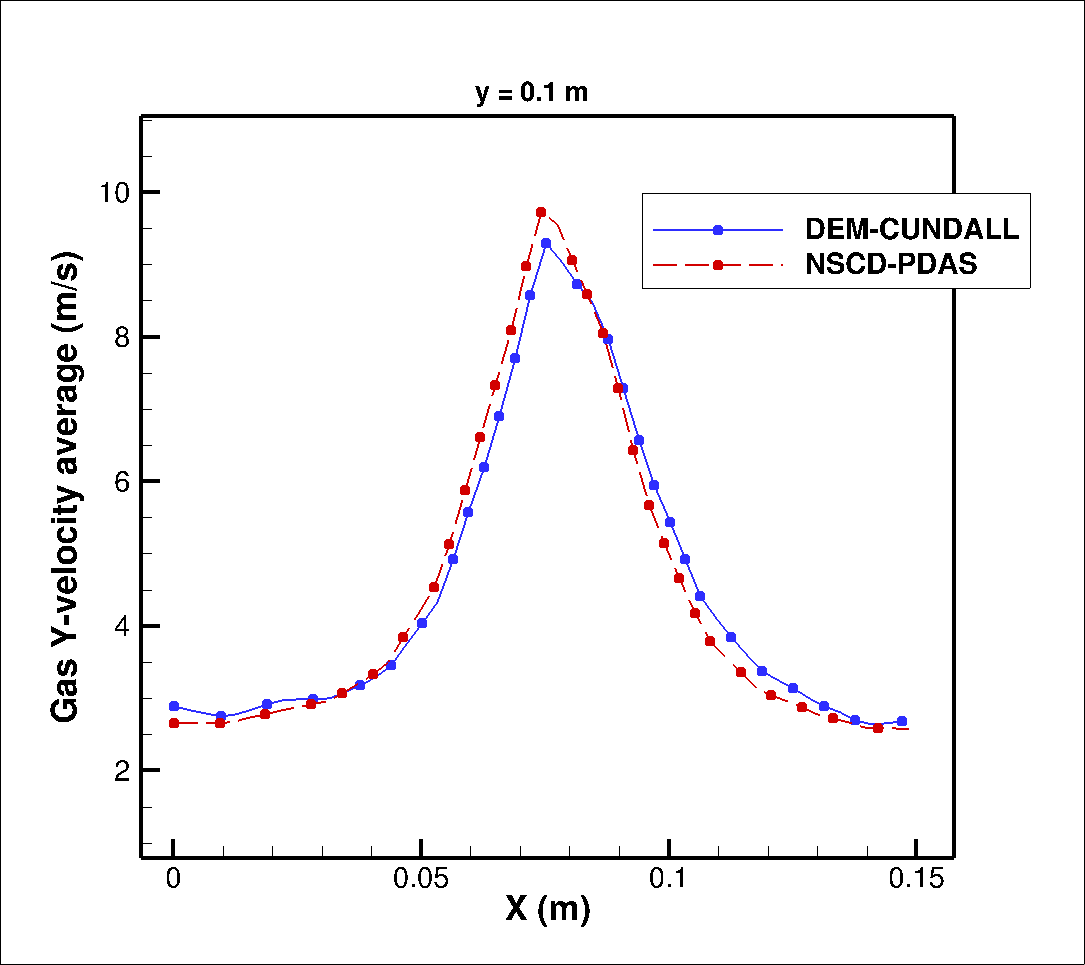
\includegraphics[trim=10 30 50 30,clip, width=0.32\textwidth]{chapitres/chapitre_4/figures/v_g_avg_data-profile_01.png}}
\hspace{\fill}
   \subfloat[\label{v_g_avg_data-profile_02} ]{%
      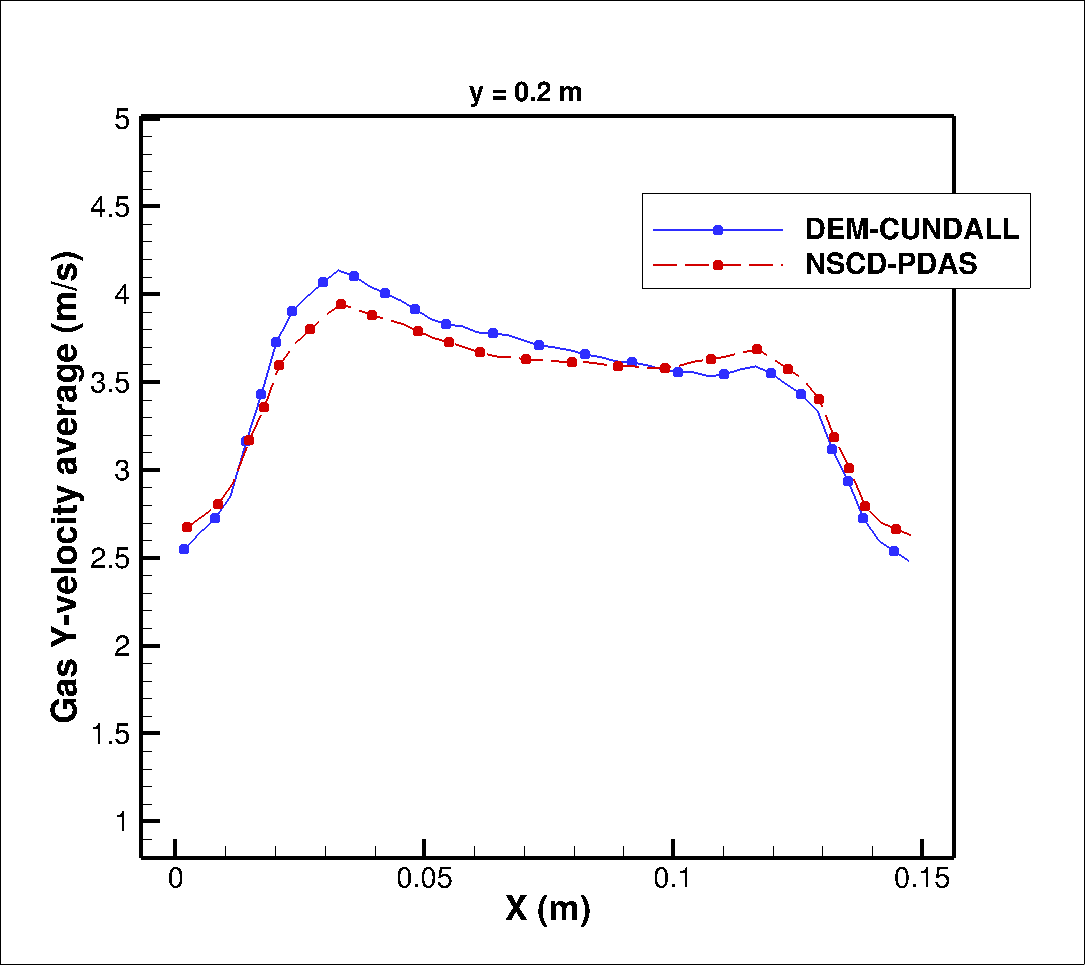
\includegraphics[trim=10 30 50 30,clip, width=0.32\textwidth]{chapitres/chapitre_4/figures/v_g_avg_data-profile_02.png}}
\hspace{\fill}
   \subfloat[\label{v_g_avg_data-profile_03} ]{%
      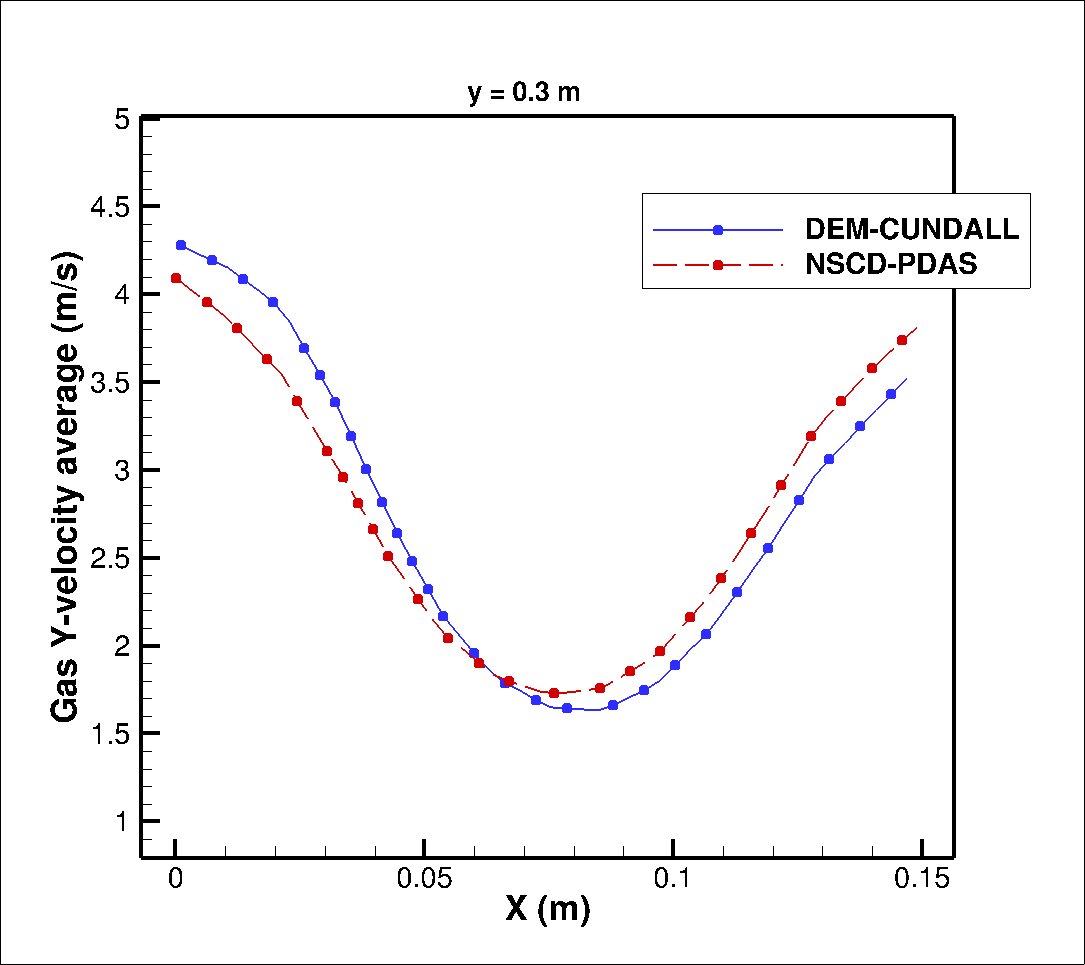
\includegraphics[trim=10 30 50 30,clip, width=0.32\textwidth]{chapitres/chapitre_4/figures/v_g_avg_data-profile_03.png}}\\
\caption{\label{v_g_avg_data-profile}Profils de vitesse d'écoulement du fluide moyennés dans le temps obtenus pour le lit fluidisé de Goldschmidt à différentes hauteurs. (a) $0.1 m$, (b) $0.2 m$, (c) $0.3 m$.}
\end{figure*}

On notera également que les hauteurs moyennes du lit, déterminées à partir des hauteurs moyennes maximales des particules, sont quasiment identiques. Ainsi, le modèle CFD couplé aux deux approches DEM-CUNDALL et NSCD-PDAS fournit des résultats proches.

\subsubsection{Caractère implicite de la NSCD}

Nous considérons à présent une comparaison des deux approches en terme de temps CPU pour atteindre $60s$ de simulation. Pour cela, nous réalisons trois autres simulations  (deux en DEM-CUNDALL en prenant des $k_n$ à $10^4$ et $10^6$ $N.m^{-1}$ et une en NSCD-PDAS avec un pas de temps solide plus grand: $dt_{solide} = 5\times10^{-4} s$), en plus de celles présentées précédemment. Pour l'approche DEM-CUNDALL, nous faisons varier la constante $k_n$ de façon à garder une dynamique de contact et un mouvement de particules réaliste, tout en essayant d'obtenir des temps de calcul solides raisonnables. Dans la Table \ref{tab_cpu_lit}, nous fournissons les temps CPU totaux fluide et solide pour chaque simulation.

\begin{table}[!h]
\begin{tabular}{|p{6.5cm}|p{3.1cm}|p{3.1cm}|}
  \hline \rowcolor{lightgray}
  Approche de contact & Temps CPU total fluide (s) & Temps CPU total solide (s)\\ 
  \hline  DEM-CUNDALL ($k_n = 2519$ $N.m^{-1}$) & $3019$ & $20050$\\
  DEM-CUNDALL ($k_n = 10^4$ $N.m^{-1}$) & $3033$ & $38230$\\
  DEM-CUNDALL ($k_n = 10^6$ $N.m^{-1}$) & $3054$ & $346103$\\
  NSCD-PDAS ($dt_{solide} = 1\times10^{-4}$ $s$)& $3039$ & $132081$\\ 
  NSCD-PDAS ($dt_{solide} = 5\times10^{-4}$ $s$)& $3022$ & $21302$\\ 
 \hline
\end{tabular}
 \caption{Temps CPU totaux fluide et solide pour simuler le lit de Goldschmidt selon l'approche de contact.}\label{tab_cpu_lit}
\end{table}

\begin{figure}[!h]
  \centering
    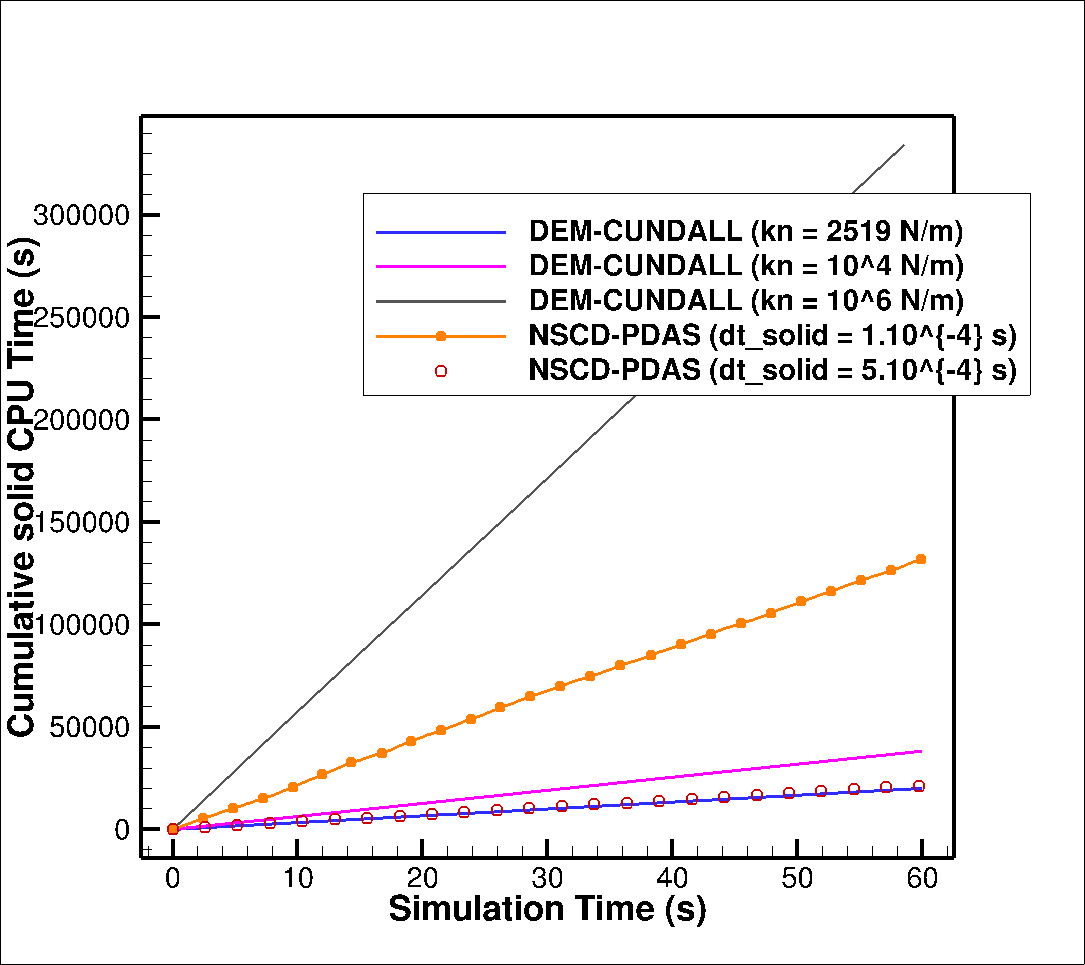
\includegraphics[width=0.6\textwidth]{chapitres/chapitre_4/figures/cumul_solid_cpu_time.png}
    \caption{\centering Évolution du temps CPU solide cumulé nécessaire pour calculer les impulsions de contact lors de la simulation du lit fluidisé de Goldschmidt pour chaque approche de contact et différents paramètres numériques.}\label{cumul_solid_cpu_time}
\end{figure}

Les résultats ainsi obtenus nous conduisent à dire que pour des valeurs de $k_n$ relativement faibles (d'ordre $\le 10^4)$, les temps CPU solides sont moins importants que ceux obtenus avec l'approche NSCD-PDAS avec un pas de temps solide $dt_{solide} = 1\times10^{-4} s$. À partir d'une valeur de $k_n = 10^6 N.m^{-1}$, ils deviennent supérieurs à l'approche NSCD-PDAS qui nous permet de choisir des pas de temps solides beaucoup plus grands et proches des pas de temps fluides, en l'occurence $dt_{solide} = 5\times10^{-4} s$. Nous pouvons affirmer à partir des valeurs de la Table \ref{tab_cpu_lit} qu'au delà d'une valeur de $k_n$ d'ordre $10^6 N.m^{-1}$,  les temps de calcul  sont trop important et ne sont plus comparables à ceux obtenus par DEM-CUNDALL avec un $k_n$ plus petit ou par NSCD-PDAS avec un $dt_{solide} = 5\times10^{-4} s$. Le graphe de la Figure \ref{cumul_solid_cpu_time} permet de confirmer cette tendance. Plus le $k_n$ est grand, plus l'écart de temps CPU solide s'élargit pour l'approche DEM-CUNDALL, tandis que plus le pas de temps est grand pour l'approche NSCD-PDAS, plus les temps de calculs sont meilleurs et proches de ceux obtenus avec un $k_n$ faible.\\

Pour conclure ce paragraphe, nous traçons dans les graphes \ref{nscd_cumul_nlgs_per_fluid_1s} et \ref{nscd_cumul_nlgs_per_fluid_60s} l'évolution au cours du temps des itérations NLGS cumulées par pas de temps fluide sur 1 s et 60 s de simulation respectivement obtenue par NSCD-PDAS en prenant deux pas de temps différents, l'un étant $5$ fois plus grand que l'autre. Ainsi, entre deux pas de temps fluide, on peut prendre plusieurs pas de temps solide. Or le caractère implicite de la NSCD nous permet de choisir des pas de temps solides plus grand, et on constate qu'en prenant un pas de temps solide $5$ fois plus grand, on limite fortement le nombre d'itérations NLGS cumulées en ayant le même résultat. Ce qui explique en grande partie le gain en temps CPU total solide observé dans la Table \ref{tab_cpu_lit} et le graphe de la Figure \ref{cumul_solid_cpu_time}.

\begin{figure*}[h!]
   \subfloat[\label{nscd_cumul_nlgs_per_fluid_1s}]{%
      \includegraphics[width=0.5\textwidth]{chapitres/chapitre_4/figures/nscd_cumul_nlgs_per_fluid_1s.png}}
\hspace{\fill}
   \subfloat[\label{nscd_cumul_nlgs_per_fluid_60s} ]{%
      \includegraphics[width=0.5\textwidth]{chapitres/chapitre_4/figures/nscd_cumul_nlgs_per_fluid_60s.png}}\\
\caption{Évolution au cours du temps des itérations NLGS cumulés par pas de temps fluide (a) sur 1 s de simulation, (b) sur 60 s de simulation obtenus par NSCD-PDAS avec deux pas de temps solides différents.}\label{nscd_cumul_nlgs_per_fluid}
\end{figure*}

L'ensemble de ces éléments nous permettent d'affirmer que le caractère implicite de la NSCD contribue à la réduction des temps de simulations d'un point de vue mise en oeuvre pratique.

\newpage

\section*{Conclusion}

Dans ce chapitre, nous démontrons la pertinence de la méthode NSCD-PDAS dans un cadre applicatif. Ce dernier est directement hérité du solveur open source MFiX-EXA qui nous a permis de réaliser des simulations d'écoulement granulaire sur une architecture multi-processeurs dans un tambour d'une part, et d'autre part, une simulation d'écoulement dans un lit fluidisé.
De plus, ce choix nous a permis de réaliser des comparaisons avec le modèle commun régularisé DEM-CUNDALL et ce, sur l'ensemble des simulations réalisées couvrant des aspects académiques et appliqués.\\

Ainsi, après avoir détaillé les lois gouvernant la dynamique des milieux granulaires dans le cadre de la DEM, nous avons décris l'implémentation du formalisme numérique NSCD-PDAS dans le solveur d'écoulements multiphasiques MFiX-EXA. Cet environnement de développement généraliste et massivement parallèle nous a permis de réaliser des comparaisons applicatives DEM/NSCD, en plus d'étendre la NSCD au couplage fluide-particules.\\
Dans cette perspective, nous avons envisagé l'implémentation de l'approche NSCD-PDAS dans le cadre du calcul parallèle du fait des coûts de calculs très importants pour des applications type industriels. Nous avons ainsi pu établir des comparaisons applicatives entre les deux approches DEM-CUNDALL et NSCD-PDAS sur des simulations d'écoulements granulaires purs, puis nous avons étendu ces comparaisons à des simulations couplées au fluide, tels que le lit fluidisé, afin d'étudier l'influence des interactions fluides-particules sur l'écoulement, tout en considérant des interactions particules-particules type NSCD, différentes de ce qui se fait dans la littérature.\\ 

Premièrement, les comparaisons numériques établies sur les cas-tests d'écoulements granulaires purs indiquent des comportements voisins des deux approches, notamment en terme de profils d'écoulement. De plus, dans le cas du tambour, la NSCD assure à la fois une non-interpénétrabilité et une conservation de la quantité d’énergie en régime établi, même si les temps de calcul y sont beaucoup plus important en raison du grand nombre d'itérations non-linéaires, en comparaison avec l’approche DEM-CUNDALL. Pour ce qui est des performances de parallélisation, les résultats obtenus ne sont pas satisfaisants dans le sens où le paradigme de décomposition de domaine géométrique proposé par MFiX-EXA n'est pas adapté aux écoulements denses tels que le tambour rotatif, et génère des pertes d'efficacité en terme de rapidité de calculs aussi bien pour l'approche DEM-CUNDALL que pour la NSCD-PDAS.\\

Deuxièmement, les simulations réalisées sur le lit fluidisé de Goldschmidt nous ont permis de mettre en avant la pertinence et la validité de l'approche NSCD-PDAS sur des écoulements granulaires couplés au fluide. 
La comparaison des champs et des profils d'écoulement de certaines variables quantitatives relatives au fluide moyennées dans le temps nous a permis de constater une variation similaire pour les deux approches. De plus, le caractère implicite de la NSCD permettant de relaxer les pas de temps solides est à l'origine des gains en temps de calcul comparé à l'approche DEM-CUNDALL restrictive à ce niveau là. On peut également évoquer le fait que les écoulements fluides-particules présentent très peu de sédimentation, ce qui se traduit notamment par une convergence non-linéaire plus rapide. Tous ces éléments nous poussent à envisager des solveurs fluides implicites, où l'on pourrait avoir un pas de temps solide pour un pas de temps fluide, limitant ainsi le nombre d'itérations non-linéaires.